\chapter[\index{topological space@Topological space}\index{topological space@Topological space}Topological Spaces \index{Quotient topology!and continuous functions}\index{Quotient topology!and continuous functions}and Continuous Functions]{Topological Spaces \\and Continuous Functions}
\vspace{6.5cm}

The concept of topological \index{First-countable space (see First-countability)} space grew out of the study of the real line and euclidean space and the study of \index{continuous function} on these spaces. In this chapter, we define what a \index{Topological space}\index{Topological space}topological space is, and we study a number of ways of constructing a \index{topology} on a set so as to make it into a topological space. We also consider some of the elementary concepts associ\index{Continuity: of algebraic operations in \(\mathbb{R}\)!at a point}\index{Continuity: of algebraic operations in \(\mathbb{R}\)!at a point}ated with topological spaces. Open and \index{closed set}, \index{limit point}, \index{Quotient topology!and continuous functions}\index{Quotient topology!and continuous functions}\index{Sequences!and closure}and cont\index{Closure!in a cartesian product}inuous functions are introduced as natural \index{Cartesian product: countably infinite!general}\index{Cartesian product: countably infinite!general}\index{Cartesian product: countably infinite!general}\index{Cartesian product: countably infinite!general}generalizations of the corresponding ideas for the real line and euclidean space.

\section*{§ 12 Topological Spaces}

The definition of a topological space that is now \index{Standard topology: on} standard was a long time in being formulated. Various mathematicians-Fréchet, Hausdorff, and others-proposed different definitions over a period of years during the first decades of the twentieth century, but it took quite a while before mathematicians settled on the one that seemed most suitable. They wanted, of course, a definition that was as broad as possible, so that it would include as special cases all the various examples that were useful in mathematics-euclidean space, \index{infinite series} infinite-dimensional euclidean space, and function spaces among them-but they also wanted the definition to be narrow enough that the standard theorems about these familiar spaces would hold for topological spaces in general. This is always the problem when one is trying to formulate a new mathematical concept, to decide how general its definition should be. The definition finally settled on may seem a bit abstract, but as you work through the various ways of constructing topological spaces, you will get a better feeling for what the concept means.

\begin{definition}
	A \index{Topology}\index{Topology}\index{topology@Topology}\index{topology@Topology}topology on a set \(X\) is a collection \(\mathcal{T}\) of subsets of \(X\) having the following properties:

(1) \(\varnothing\) and \(X\) are in \(\mathcal{T}\) .

(2) The union of the elements of any subcollection of \(\mathcal{T}\) is in \(\mathcal{T}\) .

(3) The intersection of the elements of any finite subcollection of \(\mathcal{T}\) is in \(\mathcal{T}\) .

A set \(X\) for which a topology \(\mathcal{T}\) has been specified is called a topological space.

Properly speaking, a topological space is an \index{Ray in ordered set} ordered pair(X, T)consisting \index{Interior point: of an arc!of a set}\index{Interior point: of an arc!of a set}\index{Interior point: of an arc!of a set}\index{Interior point: of an arc!of a set}of a set \(X\) and a topology \(\mathcal{T}\) on \(X\) , but we often omit specific mention of \(\mathcal{T}\) if no confusion will anse.
\end{definition}


If \(X\) is a topological space with topology \(\mathcal{T}\) , we say that a subset \(U\) of \(X\) is an \index{open set} of \(X\) if \(U\) belongs to the collection \(\mathcal{T}\) . Using this terminology, one can say that a topological space is a set \(X\) together with a collection of subsets of \(X\) , called \index{Open set}\index{Open set}\index{open set@Open set}\index{open set@Open set}open sets, such that \(\varnothing\) and \(X\) are both open, and such that arbitrary unions and finite intersections of open sets are open.

\begin{centeredblock}
\begin{example}
	Let \(X\) be a three-element set, \(X = \{ a,b,c\}\) There are many possible topologies on \(X\) , some of which are indicated schematically in Figure 12.1. The diagram in the upper right-hand corner indicates the topology in which the open sets are \(X,\varnothing\) , \(\{ a,b\} ,\{ b\}\) , and \(\{ b,c\}\) The topology in the upper left-hand corner contains only \(X\) and \(\varnothing\) , while the topology in the lower right-hand corner contains every subset \index{Comparability: of cardinalities!of topologies}\index{Comparability: of cardinalities!of topologies}of \(X\) . You can get other topologies on \(X\) by permuting \(a,b\) , and \(c\)

\begin{center}
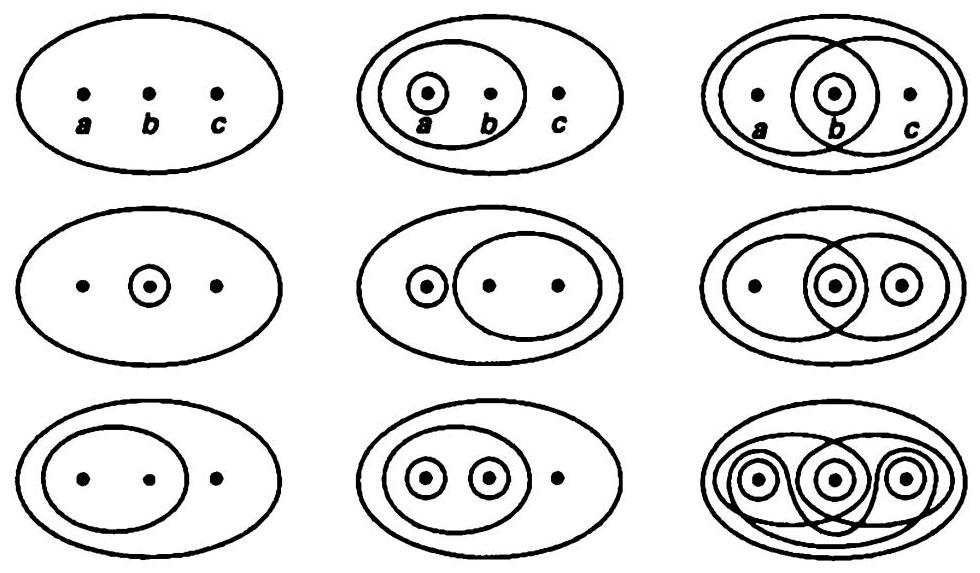
\includegraphics[width=0.9\textwidth]{images/12.1.jpg}
\end{center}
\hspace*{3em}

Figure 12.1
\end{example}
\end{centeredblock}

From this example, you can see that even a three-element set has many different topologies. But not every collection of subsets of \(X\) is a topology on \(X\) Neither of the collections inducated in Figure 122 is a topology, for instance.

\begin{center}
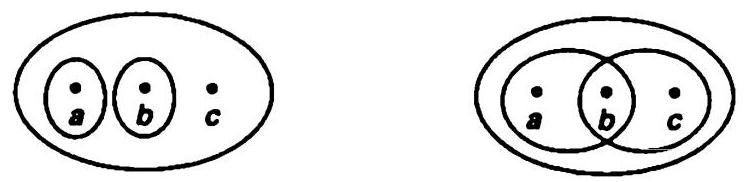
\includegraphics[width=0.6\textwidth]{images/12.2.jpg}
\end{center}
\hspace*{3em}

Figure 12.2

\begin{centeredblock}
\begin{example}
	If \(X\) is any set, the collection of all subsets of \(X\) is a topology on \(X\) , it is called the \index{discrete topology} The collection consisting of \(X\) and \(\varnothing\) only is also a topology on \(X\) ; we shall call it the \index{indiscrete topology}, or the \index{trivial topology}
\end{example}
\end{centeredblock}

\begin{centeredblock}
\begin{example}
	Let \(X\) be a set, let \({\mathcal{T}}_{f}\) be the collection of all subsets \(U\) of \(X\) such that \(X - U\) either is finite or is all of \(X\) Then \({\mathcal{T}}_{f}\) is a topology on \(X\) , called the \index{finite complement topology}. Both \(X\) and \(\varnothing\) are in \({\mathcal{T}}_{f}\) , since \(X - X\) is finite and \(X - \varnothing\) is all of \(X\) If \(\{  {U}_{\alpha }\}\) is an indexed family of nonempty elements of \({\mathcal{T}}_{f}\) , to show that \(\bigcup {U}_{\alpha }\) is in \({\mathcal{T}}_{f}\) , we compute

\[
X - \bigcup {U}_{\alpha } = \bigcap ( {X - {U}_{\alpha }})
\]

The latter set is finite because each set \(X - {U}_{\alpha }\) is finite If \({U}_{1},\;,{U}_{n}\) are nonempty elements of \({\mathcal{T}}_{f}\) , to show that \(\bigcap {U}_{t}\) is in \({\mathcal{T}}_{f}\) , we compute

\[
X - \mathop{\bigcap }\limits_{{i = 1}}^{n}{U}_{i} = \mathop{\bigcup }\limits_{{i = 1}}^{n}( {X - {U}_{i}})
\]

The latter set is a finite union of finite sets and, therefore, finite
\end{example}
\end{centeredblock}

\begin{centeredblock}
\begin{example}
	Let \(X\) be a set, let \({\mathcal{T}}_{c}\) be the collection of all subsets \(U\) of \(X\) such that \(X - U\) either is \index{Countable basis at a point} countable or is all of \(X\) . Then \({\mathcal{T}}_{c}\) is a topology on \(X\) , as you can check
\end{example}
\end{centeredblock}

\begin{definition}
	Suppose that \(\mathcal{T}\) and \({\mathcal{T}}^{\prime }\) are two topologies on a given set \(X\) . If \({\mathcal{T}}^{\prime } \supset  \mathcal{T}\) , we say that \({\mathcal{T}}^{\prime }\) is \index{Finer topology} finer than \(\mathcal{T}\) ; if \({\mathcal{T}}^{\prime }\) properly contains \(\mathcal{T}\) , we say that \({\mathcal{T}}^{\prime }\) is \index{Strictly coarser topology} strictly finer than \(\mathcal{T}\) . We also say that \(\mathcal{T}\) is \index{Coarser topology} coarser than \({\mathcal{T}}^{\prime }\) , or strictly coarser, in these two respective situations. We say \(\mathcal{T}\) is comparable with \({\mathcal{T}}^{\prime }\) if either \({\mathcal{T}}^{\prime } \supset  \mathcal{T}\) or \(\mathcal{T} \supset  {\mathcal{T}}^{\prime }\) .
\end{definition}


This terminology is suggested by thinking of a topological space as being something like a truckload full \index{Closure!of a union}\index{Closure!of a union}of gravel--the pebbles and all unions of collections of pebbles being the open sets. If now we smash the pebbles into \index{Smaller topology} \index{smaller topology@Smaller topology}\index{smaller topology@Smaller topology}smaller ones, the collection of open sets has been enlarged, and the topology, like the gravel, is said to have been made finer by the operation.

Two topologies on \(X\) need not be comparable, of course. In Figure 121 preceding, the topology in the upper right-hand corner is strictly finer than each of the three topologies in the first column and strictly coarser than each of the other topologies in the third column. But it is not comparable with any of the topologies in the second column.

Other terminology is sometimes used for this concept. If \({\mathcal{T}}^{\prime } \supset  \mathcal{T}\) , some mathematicians would say that \({\mathcal{T}}^{\prime }\) is \index{Larger topology} larger than \(\mathcal{T}\) , and \(\mathcal{T}\) is smaller than \({\mathcal{T}}^{\prime }\) . This is certainly acceptable terminology, if not as vivid as the words ``\index{finer topology@Finer topology}finer'' and ``\index{coarser topology@Coarser topology}\index{coarser topology@Coarser topology}coarser.''

Many mathematicians use the words ``\index{Weaker topology} \index{weaker topology@Weaker topology}\index{weaker topology@Weaker topology}weaker'' and ``\index{Stronger topology} stronger'' in this context. Unfortunately, some of them (particularly analysts) are apt to say that \({\mathcal{T}}^{\prime }\) is stronger than \(\mathcal{T}\) if \({\mathcal{T}}^{\prime } \supset  \mathcal{T}\) , while others (particularly topologists) are apt to say that \({\mathcal{T}}^{\prime }\) is weaker than \(\mathcal{T}\) in the same situation! If you run across the terms ``strong topology'' or ``weak topology'' in some book, you will have to decide from the context which inclusion is meant. We shall not use these terms in this book.

\section*{§ 13 Basis for a Topology}

For each of the examples in the preceding section, we were able to specify the topology by describing the entire collection \(\mathcal{T}\) of open sets. Usually this is too difficult. In most cases, one specifies instead a smaller collection of subsets of \(X\) and defines the topology in terms of that.

\begin{definition}
	If \(X\) is a set, a \index{Box topology!basis for}\index{Box topology!basis for}\index{Box topology!basis for}\index{Box topology!basis for}basis for a topology on \(X\) is a collection \(\mathcal{B}\) of subsets of \(X\) (called basis elements) such that

(1) For each \(x \in  X\) , there is at least one basis element \(B\) containing \(x\) .

(2) If \(x\) belongs to the intersection of two basis elements \({B}_{1}\) and \({B}_{2}\) , then there is a basis element \({B}_{3}\) containing \(x\) such that \({B}_{3} \subset  {B}_{1} \cap  {B}_{2}\) .

If \(\mathcal{B}\) satisfies these two conditions, then we define the topology \(\mathcal{T}\) generated by \(\mathcal{B}\) as follows: \(A\) subset \(U\) of \(X\) is said to be open in \(X\) (that is, to be an element of \(\mathcal{T}\) ) if for each \(x \in  U\) , there is a basis element \(B \in  \mathcal{B}\) such that \(x \in  B\) and \(B \subset  U\) . Note that each basis element is itself an element of \(\mathcal{T}\) .
\end{definition}

We will check shortly that the collection \(\mathcal{T}\) is indeed a topology on \(X\) . But first let us consider some examples.


\begin{centeredblock}
\begin{example}
	Let \(\mathcal{B}\) be the collection of all circular regions (interiors of circles) in the plane. Then \(\mathcal{B}\) satisfies both conditions for a basis The second condition is illustrated in Figure 13 1. In the topology generated by \(\mathcal{B}\) , a subset \(U\) of the plane is open if every \(x\) in \(U\) lies in some circular region contained in \(U\)

\begin{center}
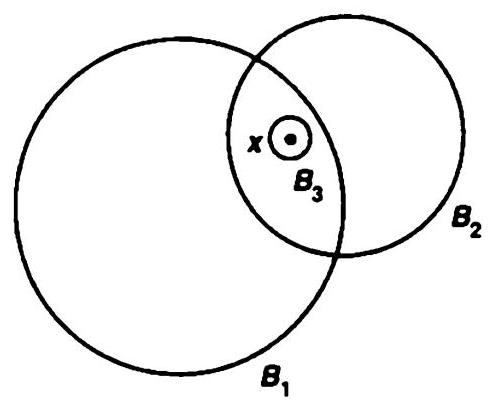
\includegraphics[width=0.4\textwidth]{images/13.1.jpg}
\end{center}
\hspace*{3em}

Figure 13.1

\begin{center}
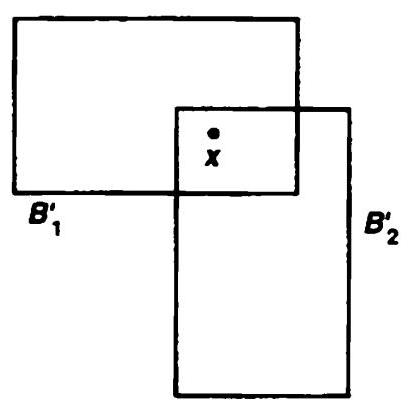
\includegraphics[width=0.3\textwidth]{images/13.2.jpg}
\end{center}
\hspace*{3em}

Figure 13.2
\end{example}
\end{centeredblock}

\begin{centeredblock}
\begin{example}
	Let \({\mathcal{B}}^{\prime }\) be the collection of all rectangular regions (interiors of rectangles) in the plane, where the rectangles have sides parallel to the \index{Coordinate: of J-tuple} coordinate axes Then \({\mathcal{B}}^{\prime }\) satisfies both conditions for a basis. The second condition is illustrated in Figure 132; in thus case, the condition is tri\index{Closure!via basis elements}\index{Closure!via basis elements}vial, because the intersection of any two basis elements is itself a basis element (or empty) As we shall see later, the basis \({\mathcal{B}}^{\prime }\) generates the same topology on the plane as the basis \(\mathcal{B}\) given in the preceding example
\end{example}
\end{centeredblock}

\begin{centeredblock}
\begin{example}
	If \(X\) is any set, the collection \index{Continuity: of algebraic operations in \(\mathbb{R}\)!of metric}of all one-point subsets of \(X\) is a basis \index{Metric!for discrete topology}\index{Metric!for discrete topology}for the \index{Discrete topology}\index{Discrete topology}\index{discrete topology@Discrete topology}\index{discrete topology@Discrete topology}discrete topology on \(X\)
\end{example}
\end{centeredblock}

Let us check now that the collection \(\mathcal{T}\) generated by the basis \(\mathcal{B}\) is, in fact, a topology on \(X\) . If \(U\) is the empty set, it satisfies the defining condition of openness vacuously. Likewise, \(X\) is in \(\mathcal{T}\) , since for each \(x \in  X\) there is some basis element \(B\) containing \(x\) and contained in \(X\) Now let us take an indexed family \({\{  {U}_{\alpha }\}  }_{\alpha  \in  J}\) , of elements of \(\mathcal{T}\) and show that

\[
U = \mathop{\bigcup }\limits_{{\alpha  \in  J}}{U}_{\alpha }
\]

belongs to \(\mathcal{T}\) . Given \(x \in  U\) , there is an index \(\alpha\) such that \(x \in  {U}_{\alpha }\) . Since \({U}_{\alpha }\) is open, there is a basis element \(B\) such that \(x \in  B \subset  {U}_{\alpha }\) . Then \(x \in  B\) and \(B \subset  U\) , so that \(U\) is open, by definition.

Now let us take two elements \({U}_{1}\) and \({U}_{2}\) of \(\mathcal{T}\) and show that \({U}_{1} \cap  {U}_{2}\) belongs to \(\mathcal{T}\) . Given \(x \in  {U}_{1} \cap  {U}_{2}\) , choose a basis element \({B}_{1}\) containing \(x\) such that \({B}_{1} \subset  {U}_{1}\) ; choose also a basis element \({B}_{2}\) containing \(x\) such that \({B}_{2} \subset  {U}_{2}\) . The second condition for a basis enables us to choose a basis element \({B}_{3}\) containing \(x\) such that \({B}_{3} \subset  {B}_{1} \cap  {B}_{2}\) . See Figure 13.3. Then \(x \in  {B}_{3}\) and \({B}_{3} \subset  {U}_{1} \cap  {U}_{2}\) , so \({U}_{1} \cap  {U}_{2}\) belongs to \(\mathcal{T}\) , by definition.

\begin{center}
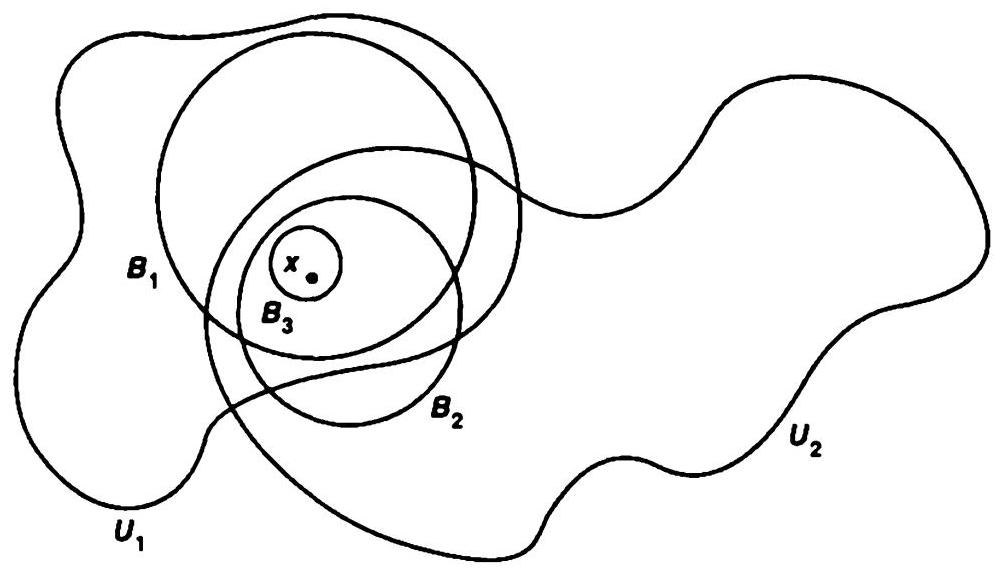
\includegraphics[width=0.9\textwidth]{images/13.3.jpg}
\end{center}
\hspace*{3em} 

Figure 13.3

Finally, we show by induction that any finite intersection \({U}_{1} \cap  \cdots  \cap  {U}_{n}\) of elements of \(\mathcal{T}\) is in \(\mathcal{T}\) . This fact is trivial for \(n = 1\) ; we suppose it true for \(n - 1\) and prove it for \(n\) . Now

\[
( {{U}_{1} \cap   \cdot   \cap  {U}_{n}})  = ( {{U}_{1} \cap  \cdots  \cap  {U}_{n - 1}})  \cap  {U}_{n}
\]

By hypothesis, \({U}_{1} \cap   \cdot   \cdot   \cap  {U}_{n - 1}\) belongs to \(\mathcal{T}\) ; by the result just proved, the intersection of \({U}_{1} \cap  \cdots  \cap  {U}_{n - 1}\) and \({U}_{n}\) also belongs to \(\mathcal{T}\)

Thus we have checked that collection of open sets \index{Topology!generated by a basis}\index{Topology!generated by a basis}\index{Topology!generated by a basis}\index{Topology!generated by a basis}generated by a basis \(\mathcal{B}\) is, in fact, a topology.

Another way of describing the topology generated by a basis is given in the following lemma.

\begin{lemma}
	Let \(X\) be a set; let \(\mathcal{B}\) be a basis for a topology \(\mathcal{T}\) on \(X\) . Then \(\mathcal{T}\) equals the collection of all unions of elements of \(\mathcal{B}\) .
\end{lemma}

\begin{proof}
Given a collection of elements of \(\mathcal{B}\) , they are also elements of \(\mathcal{T}\) . Because \(\mathcal{T}\) is a topology, their union is in \(\mathcal{T}\) . Conversely, given \(U \in  \mathcal{T}\) , choose for each \(x \in  U\) an element \({B}_{x}\) of \(\mathcal{B}\) such that \(x \in  {B}_{x} \subset  U\) . Then \(U = \mathop{\bigcup }\limits_{{x \in  U}}{B}_{x}\) , so \(U\) equals a union of elements of \(\mathcal{B}\) .

This lemma states that every open set \(U\) in \(X\) can be expressed as a union of basis elements. This expression for \(U\) is not, however, unique. Thus the use of the term ``basis'' in topology differs drastically from its use in linear algebra, where the equation expressing a given vector as a linear combination of basis vectors is unique.

We have described in two different ways how to go from a basis to the topology it generates. Sometimes we need to go in the reverse direction, from a topology to a basis generating it. Here is one way of obtaining a basis for a given topology; we shall use it frequently.
\end{proof}

\begin{lemma}
	Let \(X\) be a topological space. Suppose that \(\mathcal{C}\) is a collection of open sets of \(X\) such that for each open set \(U\) of \(X\) and each \(x\) in \(U\) , there is an element \(C\) of \(\mathcal{C}\) such that \(x \in  C \subset  U\) . Then \(\mathcal{C}\) is a basis for the topology of \(X\) .
\end{lemma}

\begin{proof}
We must show that \(\mathcal{C}\) is a basis. The first condition for a basis is easy: Given \(x \in  X\) , since \(X\) is itself an open set, there is by hypothesis an element \(C\) of \(\mathcal{C}\) such that \(x \in  C \subset  X\) . To check the second condition, let \(x\) belong to \({C}_{1} \cap  {C}_{2}\) , where \({C}_{1}\) and \({C}_{2}\) are elements of \(\mathcal{C}\) . Since \({C}_{1}\) and \({C}_{2}\) are open, so is \({C}_{1} \cap  {C}_{2}\) . Therefore, there exists by hypothesis an element \({C}_{3}\) in \(\mathcal{C}\) such that \(x \in  {C}_{3} \subset  {C}_{1} \cap  {C}_{2}\) .

Let \(\mathcal{T}\) be the collection of open sets of \(X\) ; we must show that the topology \({\mathcal{T}}^{\prime }\) generated by \(\mathcal{C}\) equals the topology \(\mathcal{T}\) . First, note that if \(U\) belongs to \(\mathcal{T}\) and if \(x \in  U\) , then there is by hypothesis an element \(C\) of \(\mathcal{C}\) such that \(x \in  C \subset  U\) . It follows that \(U\) belongs to the topology \({\mathcal{T}}^{\prime }\) , by definition. Conversely, if \(W\) belongs to the topology \({\mathcal{T}}^{\prime }\) , then \(W\) equals a union of elements of \(\mathcal{C}\) , by the preceding lemma. Since each element of \(\mathcal{C}\) belongs to \(\mathcal{T}\) and \(\mathcal{T}\) is a topology, \(W\) also belongs to \(\mathcal{T}\) .

When topologies are given by bases, it is useful to have a criterion in terms of the bases for determining whether one topology is finer than another. One such criterion is the following.
\end{proof}

\begin{lemma}
	Let \(\mathcal{B}\) and \({\mathcal{B}}^{\prime }\) be bases for the topologies \(\mathcal{T}\) and \({\mathcal{T}}^{\prime }\) , respectively, on \(X\) . Then the following are equivalent:

(1) \({\mathcal{T}}^{\prime }\) is finer than \(\mathcal{T}\) .

(2) For each \(x \in  X\) and each basis element \(B \in  \mathcal{B}\) containing \(x\) , there is a basis element \({B}^{\prime } \in  {\mathcal{B}}^{\prime }\) such that \(x \in  {B}^{\prime } \subset  B\) .
\end{lemma}

\begin{proof}
(2) \(\Rightarrow\) (1). Given an element \(U\) of \(\mathcal{T}\) , we wish to show that \(U \in  {\mathcal{T}}^{\prime }\) . Let \(x \in  U\) . Since \(\mathcal{B}\) generates \(\mathcal{T}\) , there is an element \(B \in  \mathcal{B}\) such that \(x \in  B \subset  U\) . Condition (2) tells us there exists an element \({B}^{\prime } \in  {\mathcal{B}}^{\prime }\) such that \(x \in  {B}^{\prime } \subset  B\) . Then \(x \in  {B}^{\prime } \subset  U\) , so \(U \in  {\mathcal{T}}^{\prime }\) , by definition.

(1) \(\Rightarrow\) (2). We are given \(x \in  X\) and \(B \in  \mathcal{B}\) , with \(x \in  B\) . Now \(B\) belongs to \(\mathcal{T}\) by definition and \(\mathcal{T} \subset  {\mathcal{T}}^{\prime }\) by condition (1); therefore, \(B \in  {\mathcal{T}}^{\prime }\) Since \({\mathcal{T}}^{\prime }\) is generated by \({\mathcal{B}}^{\prime }\) , there is an element \({B}^{\prime } \in  {\mathcal{B}}^{\prime }\) such that \(x \in  {B}^{\prime } \subset  B\) .

Some students find this condition hard to remember. ``Which way does the inclusion go?'' they ask. It may be easier to remember if you recall the analogy between a topological space and a truckload full of gravel. Think of the pebbles as the basis elements of the topology; after the pebbles are smashed to dust, the dust particles are the basis elements of the new topology. The new topology is finer than the old one, and each dust particle was contained inside a pebble, as the criterion states.
\end{proof}

\begin{centeredblock}
\begin{example}
	One can now see that the collection \(\mathcal{B}\) of all circular regions in the plane generates the same topology as the collection \({\mathcal{B}}^{\prime }\) of all rectangular regions, Figure 134 illustrates the pro\\index{Subspace topology!in metric space}index{First-countability!of metric space}\index{First-countability!of metric space}of We shall treat this example more \\index{Convergent sequence!in Hausdorff space}index{Hausdorff condition!for metric space}\index{Hausdorff condition!for metric space}formally when we study \\\index{Closure!in a subspace}index{Subspace topology!in metric space}index{\index{metric space@Metric space}metric space}

\begin{center}
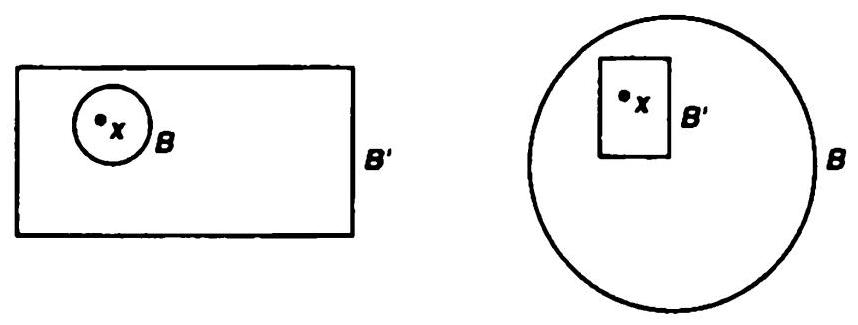
\includegraphics[width=0.7\textwidth]{images/13.4.jpg}
\end{center}
\hspace*{3em}

Figure 13.4
\end{example}
\end{centeredblock}

We now define three topologies on the real line \(\mathbb{R}\) , all of which are of interest.

\begin{definition}
	If \(\mathcal{B}\) is the collection of all open intervals in the real line,

\[
( {a,b})  = \{ x \mid  a < x < b\} ,
\]

the topology generated by \(\mathcal{B}\) is called the \index{\(\mathbb{R}\) (reals)!standard topology}\index{\(\mathbb{R}\) (reals)!standard topology}\index{\(\mathbb{R}\) (reals)!standard topology}\index{\(\mathbb{R}\) (reals)!standard topology}standard topology on the real line. Whenever we consider \(\mathbb{R}\) , we shall suppose it is given this topology unless we specifically state otherwise.
\end{definition}


If \({\mathcal{B}}^{\prime }\) is the collection of all \index{half-open interval} of the form

\[
\lbrack a,b) = \{ x \mid  a \leq  x < b\} ,
\]

where \(a < b\) , the topology generated by \({\mathcal{B}}^{\prime }\) is called the lower limit topology on \(\mathbb{R}\) . When \(\mathbb{R}\) is given the lower limit topology, we denote it by \(\index{R@\({\mathbb{R}}_{\ell }\)} \index{R@${\mathbb{R}}_{\ell }$}{\mathbb{R}}_{\ell }\) . Finally let \(K\) denote the set of all numbers of the form \(1/n\) , for \(n \in  {\mathbb{Z}}_{ + }\) , and let \({\mathcal{B}}^{\prime \prime }\) be the collection of all open intervals(a, b), along with all sets of the form \(( {a,b})  - K\) . The topology generated by \({\mathcal{B}}^{\prime \prime }\) will be called the \(K\) -topology on \(\mathbb{R}\) . When \(\mathbb{R}\) is given this topology, we denote it by \(\index{R@\({\mathbb{R}}_{K}\)} \index{R@${\mathbb{R}}_{K}$}{\mathbb{R}}_{K}\) .

It is easy to see that all three of these collections are bases; in each case, the intersection of two basis elements is either another basis element or is empty. The relation between these topologies is the following

\begin{lemma}
	The topologies of \({\mathbb{R}}_{\ell }\) and \({\mathbb{R}}_{K}\) are strictly finer than the standard topology on \(\mathbb{R}\) , but are not comparable with one another.
\end{lemma}

Proof Let \(\mathcal{T},{\mathcal{T}}^{\prime }\) , and \({\mathcal{T}}^{\prime \prime }\) be the topologies of \(\mathbb{R},{\mathbb{R}}_{\ell }\) , and \({\mathbb{R}}_{K}\) , respectively. Given a basis element(a, b)for \(\mathcal{T}\) and a point \(x\) of(a, b), the basis element \(\lbrack x,b)\) for \({\mathcal{T}}^{\prime }\) contains \(x\) and lies in(a, b). On the other hand, given the basis element \(\lbrack x,d)\) for \({\mathcal{T}}^{\prime }\) , there is no open interval(a, b)that contains \(x\) and lies in \(\lbrack x,d)\) . Thus \({\mathcal{T}}^{\prime }\) is strictly finer than \(\mathcal{T}\)

A similar argument applies to \({\mathbb{R}}_{K}\) . Given a basis element(a, b)for \(\mathcal{T}\) and a point \(x\) of(a, b), this same interval is a basis element for \({\mathcal{T}}^{\prime \prime }\) that contains \(x\) . On the other hand, given the basis element \(B = ( {-1,1})  - K\) for \({\mathcal{T}}^{\prime \prime }\) and the point0of \(B\) , there is no open interval that contains 0 and lies in \(B\) .

We leave it to you to show that the topologies of \({\mathbb{R}}_{\ell }\) and \({\mathbb{R}}_{K}\) are not comparable.

A question may occur to you at this point. Since the topology generated by a basis \(\mathcal{B}\) may be described as the collection of arbitrary unions of elements of \(\mathcal{B}\) , what happens if you start with a given collection of sets and take finite intersections of them as well as arbitrary unions? This question leads to the notion of a \index{subbasis} for a topology

\begin{definition}
	A \index{Order topology!subbasis}subbasis \(S\) for a topology on \(X\) is a collection of subsets of \(X\) whose union equals \(X\) . The topology generated by the subbasis \(S\) is defined to be the collection \(\mathcal{T}\) of all unions of finite intersections of elements of \(\mathcal{S}\) .
\end{definition}


We must of course check that \(\mathcal{T}\) is a topology. For this purpose it will suffice to show that the collection \(\mathcal{B}\) of all finite intersections of elements of \(\mathcal{S}\) is a basis, for then the collection \(\mathcal{T}\) of all unions of elements of \(\mathcal{B}\) is a topology, by Lemma 13.1. Given \(x \in  X\) , it belongs to an element of \(\mathcal{S}\) and hence to an element of \(\mathcal{B}\) ; this is the first condition for a basis. To check the second condition, let

\[
{B}_{1} = {S}_{1} \cap  \cdots  \cap  {S}_{m}\;\text{ and }\;{B}_{2} = {S}_{1}^{\prime } \cap  \cdots  \cap  {S}_{n}^{\prime }
\]

be two elements of \(\mathcal{B}\) . Their intersection

\[
{B}_{1} \cap  {B}_{2} = ( {{S}_{1} \cap  \cdots  \cap  {S}_{m}})  \cap  ( {{S}_{1}^{\prime } \cap  \cdots  \cap  {S}_{n}^{\prime }})
\]

is also a finite intersection of elements of \(\mathcal{S}\) , so it belongs to \(\mathcal{B}\) .

\section*{Exercises}
\begin{enumerate}[itemsep=0.4em, parsep=0pt, topsep=0pt, partopsep=0pt, leftmargin=*, label=\arabic*., ref=\arabic*]
\item Let \(X\) be a topological space; let \(A\) be a subset of \(X\) . Suppose that for each \(x \in  A\) there is an open set \(U\) containing \(x\) such that \(U \subset  A\) . Show that \(A\) is open in \(X\)
\item Consider the nine topologies on the set \(X = \{ a,b,c\}\) indicated in Example 1 of §12. Compare them, that is, for each pair \index{Comparability: of cardinalities!of topologies}of topologies, determine whether they are comparable, and if so, which is the finer.
\item Show that the collection \({\mathcal{T}}_{c}\) given in Example 4 of \(§{12}\) is a topology on the set \(X\) . Is the collection \[ {\mathcal{T}}_{\infty } = \{ U \mid  X - U\text{ is infinite or empty or all of }X\} \] a topology on \(X\) ?
\item
  \begin{enumerate}[itemsep=0.2em, parsep=0pt, topsep=0pt, partopsep=0pt, leftmargin=*, label=(\alph*), align=left]
  \item If \(\{  {\mathcal{T}}_{\alpha }\}\) is a family of topologies on \(X\) , show that \(\cap  {\mathcal{T}}_{\alpha }\) is a topology on \(X\) . Is \(\bigcup {\mathcal{T}}_{\alpha }\) a topology on \(X\) ?

  \item Let \(\{  {\mathcal{T}}_{\alpha }\}\) be a family of topologies on \(X\) . Show that there is a unique smallest topology on \(X\) containing all the collections \({\mathcal{T}}_{\alpha }\) , and a unique largest topology contained in all \({\mathcal{T}}_{\alpha }\) .
  \item If \(X = \{ a,b,c\}\) , let \[ {\mathcal{T}}_{1} = \{ \varnothing ,X,\{ a\} ,\{ a,b\} \} \;\text{ and }\;{\mathcal{T}}_{2} = \{ \varnothing ,X,\{ a\} ,\{ b,c\} \} . \] Find the smallest topology containing \({\mathcal{T}}_{1}\) and \({\mathcal{T}}_{2}\) , and the largest topology contained in \({\mathcal{T}}_{1}\) and \({\mathcal{T}}_{2}\) .
  \end{enumerate}
\item Show that if \(\mathcal{A}\) is a basis for a topology on \(X\) , then the topology generated by \(\mathcal{A}\) equals the intersection of all topologies on \(X\) that contain \(\mathcal{A}\) . Prove the same if \(\mathcal{A}\) is a subbasis.
\item Show that the topologies of \({\mathbb{R}}_{\ell }\) and \({\mathbb{R}}_{K}\) are not comparable.
\item Consider the following topologies on \(\mathbb{R}\) : \({\mathcal{T}}_{1} =\) the standard topology, \({\mathcal{T}}_{2} =\) the topology of \({\mathbb{R}}_{K}\) , \({\mathcal{T}}_{3} =\) the \index{Finite complement topology}finite complement topology, \({\mathcal{T}}_{4} =\) the upper limit topology, having all sets(a, b)as basis, \({\mathcal{T}}_{5} =\) the topology having all sets \(( {-\infty ,a})  = \{ x \mid  x < a\}\) as basis. Determine, for each of these topologies, which of the others it contains.
\item
  \begin{enumerate}[itemsep=0.2em, parsep=0pt, topsep=0pt, partopsep=0pt, leftmargin=*, label=(\alph*), align=left]
  \item Apply Lemma 13.2 to show that the countable collection \[ \mathcal{B} = \{ ( {a,b})  \mid  a < b,a\text{ and }b\text{ rational }\} \] is a basis that generates the standard topology on \(\mathbb{R}\) .

  \item Show that the collection \[ \mathcal{C} = \{ \lbrack a,b) \mid  a < b,a\text{ and }b\text{ rational }\} \] is a basis that generates a topology different from the lower limit topology on \(\mathbb{R}\) .
  \end{enumerate}
\end{enumerate}
\section*{§ 14 The Order Topology}

If \(X\) is a simply ordered set, there is a standard topology for \(X\) , defined using the order relation. It is called the \index{order topology}; in this section, we consider it and study some of its properties.

Suppose that \(X\) is a set having a simple order relation \(<\) . Given elements \(a\) and \(b\) of \(X\) such that \(a < b\) , there are four subsets of \(X\) that are called the intervals determined by \(a\) and \(b\) . They are the following :

\[
( {a,b})  = \{ x \mid  a < x < b\} ,
\]

\[
(a,b\rbrack  = \{ x \mid  a < x \leq  b\} ,
\]

\[
\lbrack a,b) = \{ x \mid  a \leq  x < b\} ,
\]

\[
[  {a,b}]   = \{ x \mid  a \leq  x \leq  b\} .
\]

The notation used here is familiar to you already in the case where \(X\) is the real line, but these are intervals in an arbitrary ordered set. A set of the first type is called an open interval in \(X\) , a set of the last type is called a \index{closed interval} in \(X\) , and sets of the second and third types are called \index{Half-open interval}half-open intervals. The use of the term ``open'' in this connection suggests that open intervals in \(X\) should turn out to be open sets when we put a topology on \(X\) . And so they will.

\begin{definition}
	Let \(X\) be a set with a simple order relation; assume \(X\) has more than one element. Let \(\mathcal{B}\) be the collection of all sets of the following types:

(I) All open intervals(a, b)in \(X\) .

(2) All intervals of the form \([  {{a}_{0},b})\) , where \({a}_{0}\) is the smallest element (if any) of \(X\) .

(3) All intervals of the form \(( {a,{b}_{0}}]\) , where \({b}_{0}\) is the largest element (if any) of \(X\) . The collection \(\mathcal{B}\) is a basis for a topology on \(X\) , which is called the \index{Order topology}order topology.
\end{definition}

If \(X\) has no smallest element, there are no sets of type (2), and if \(X\) has no largest element, there are no sets of type (3).

One has to check that \(\mathcal{B}\) satisfies the requirements for a basis. First, note that every element \(x\) of \(X\) lies in at least one element of \(\mathcal{B}\) : The smallest element (if any) lies in all sets of type (2), the largest element (if any) lies in all sets of type (3), and every other element lies in a set of type (1). Second, note that the intersection of any two sets of the preceding types is again a set of one of these types, or is empty. Several cases need to be checked; we leave it to you.

\begin{centeredblock}
\begin{example}
	The standard topology on \(\mathbb{R}\) , as defined in the preceding section, is just the order topology derived from the usual order on \(\mathbb{R}\) .
\end{example}
\end{centeredblock}

\begin{centeredblock}
\begin{example}
	Consider the set \(\mathbb{R} \times  \mathbb{R}\) in the dictionary order, we shall denote the general element of \(\mathbb{R} \times  \mathbb{R}\) by \(x \times  y\) , to avoid difficulty with notation The set \(\mathbb{R} \times  \mathbb{R}\) has neither a largest nor a smallest element, so the order topology on \(\mathbb{R} \times  \mathbb{R}\) has as basis the collection of all open intervals of the form \(( {a \times  b,c \times  d})\) for \(a < c\) , and for \(a = c\) and \(b < d\) . These two types of intervals are indicated in Figure 14.1. The subcollection consisting of only intervals of the second type is also a basis for the order topology on \(\mathbb{R} \times  \mathbb{R}\) , as you can check

\begin{center}
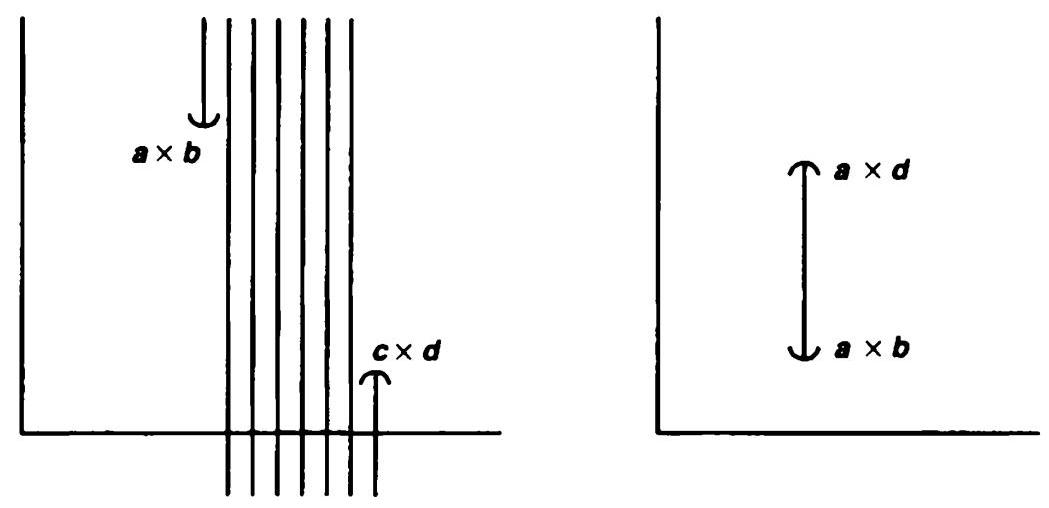
\includegraphics[width=0.9\textwidth]{images/14.1.jpg}
\end{center}
\hspace*{3em}

Figure 14.1
\end{example}
\end{centeredblock}

\begin{centeredblock}
\begin{example}
	The positive integers \({\mathbb{Z}}_{ + }\) form an ordered set with a smallest element. The order topology on \({\mathbb{Z}}_{ + }\) is the discrete topology, for every one-point set is open If \(n > 1\) , then the one-point set \(\{ n\}  = ( {n - 1,n + 1})\) is a basis element; and if \(n = 1\) , the one-point set \(\{ 1\}  = \lbrack 1,2)\) is a basis element.
\end{example}
\end{centeredblock}

\begin{centeredblock}
\begin{example}
	The set \(X = \{ 1,2\}  \times  {\mathbb{Z}}_{ + }\) in the dictionary order is another example of an ordered set with a smallest element Denoting \(1 \times  n\) by \({a}_{n}\) and \(2 \times  n\) by \({b}_{n}\) , we can represent \(X\) by

\[
{a}_{1},{a}_{2},.\;;{b}_{1},{b}_{2},\ldots
\]

The order topology on \(X\) is not the discrete topology. Most one-point sets are open, but there is an exception-the one-point set \(\{  {b}_{1}\}\) . Any open set containing \({b}_{1}\) must contain a basis element about \({b}_{1}\) (by definition), and any basis element containing \({b}_{1}\) contains points of the \({a}_{i}\) sequence.
\end{example}
\end{centeredblock}

\begin{definition}
	If \(X\) is an ordered set, and \(a\) is an element of \(X\) , there are four subsets of \(X\) that are called the rays determined by \(a\) They are the following

\[
( {a, + \infty })  = \{ x \mid  x > a\} ,
\]

\[
( {-\infty ,a})  = \{ x \mid  x < a\} ,
\]

\[
\lbrack a, + \infty ) = \{ x \mid  x \geq  a\} ,
\]

\[
( - \infty ,a\rbrack  = \{ x \mid  x \leq  a\} .
\]

Sets of the first two types are called \index{open ray}, and sets of the last two types are called \index{closed ray}.
\end{definition}

The use of the term ``open'' suggests that \index{Open ray}open rays in \(X\) are open sets in the order topology. And so they are. Consider, for example, the ray \(( {a, + \infty })\) . If \(X\) has a largest element \({b}_{0}\) , then \(( {a, + \infty })\) equals the basis element \(( {a,{b}_{0}}]\) . If \(X\) has no largest element, then \(( {a, + \infty })\) equals the union of all basis elements of the form(a, x), for \(x > a\) . In either case, \(( {a, + \infty })\) is open. A similar argument applies to the ray \(( {-\infty ,a})\) .

The open rays, in fact, form a subbasis for the order topology on \(X\) , as we now show Because the open rays are open in the order topology, the topology they generate is contained in the order topology. On the other hand, every basis element for the order topology equals a finite intersection of open rays; the interval(a, b)equals the intersection of \(( {-\infty ,b})\) and \(( {a, + \infty })\) , while \([  {{a}_{0},b})\) and \(( {a,{b}_{0}}]\) , if they exist, are themselves open rays. Hence the topology generated by the open rays contains the order topology

\section*{§ 15 The Product Topology on \(X \times  Y\)}

If \(X\) and \(Y\) are topological spaces, there is a standard way of defining a topology on the cartesian \index{Product: of continuous maps} product \(X \times  Y\) . We consider this topology now and study some of its properties.

\begin{definition}
	Let \(X\) and \(Y\) be topological spaces. The \index{product topology} on \(X \times  Y\) is the topology having as basis the collection \(\mathcal{B}\) of all sets of the form \(U \times  V\) , where \(U\) is an open subset of \(X\) and \(V\) is an open subset of \(Y\) .
\end{definition}

Let us check that \(\mathcal{B}\) is a basis. The first condition is trivial, since \(X \times  Y\) is itself a basis element. The second condition is almost as easy, since the intersection of any two basis elements \({U}_{1} \times  {V}_{1}\) and \({U}_{2} \times  {V}_{2}\) is another basis element. For

\[
( {{U}_{1} \times  {V}_{1}})  \cap  ( {{U}_{2} \times  {V}_{2}})  = ( {{U}_{1} \cap  {U}_{2}})  \times  ( {{V}_{1} \cap  {V}_{2}})
\]

and the latter set is a basis element because \({U}_{1} \cap  {U}_{2}\) and \({V}_{1} \cap  {V}_{2}\) are open in \(X\) and \(Y\) , respectively. See Figure 15.1.

Note that the collection \(\mathcal{B}\) is not a topology on \(X \times  Y\) . The union of the two rectangles pictured in Figure 15.1, for instance, is not a product of two sets, so it cannot belong to \(\mathcal{B}\) ; however, it is open in \(X \times  Y\) .

Each time we introduce a new concept, we shall try to relate it to the concepts that have been previously introduced. In the present case, we ask: What can one say if the topologies on \(X\) and \(Y\) are given by bases? The answer is as follows:

\begin{theorem}
	If \(\mathcal{B}\) is a basis for the topology of \(X\) and \(\mathcal{C}\) is a basis for the topology of \(Y\) , then the collection

\[
\mathcal{D} = \{ B \times  C \mid  B \in  \mathcal{B}\text{ and }C \in  \mathcal{C}\}
\]

is a basis for the topology of \(X \times  Y\)

\begin{center}
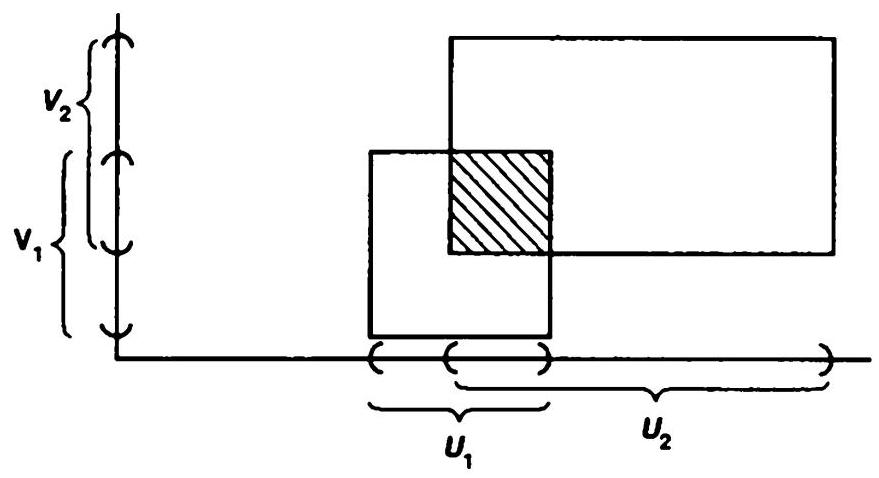
\includegraphics[width=0.8\textwidth]{images/15.1.jpg}
\end{center}
\hspace*{3em} 

Figure 15.1

\end{theorem}
\begin{proof}
We apply Lemma 13.2. Given an open set \(W\) of \(X \times  Y\) and a point \(x \times  y\) of \(W\) , by definition of the \index{Product topology}product topology there is a basis element \(U \times  V\) such that \(x \times  y \in  U \times  V \subset  W\) . Because \(\mathcal{B}\) and \(\mathcal{C}\) are bases for \(X\) and \(Y\) , respectively, we can choose an element \(B\) of \(\mathcal{B}\) such that \(x \in  B \subset  U\) , and an element \(C\) of \(\mathcal{C}\) such that \(y \in  C \subset  V\) . Then \(x \times  y \in  B \times  C \subset  W\) . Thus the collection \(\mathcal{D}\) meets the criterion of Lemma 13.2, so \(\mathcal{D}\) is a basis for \(X \times  Y\) .
\end{proof}

\begin{centeredblock}
\begin{example}
	We have a standard topology on \(\mathbb{R}\) the order topology The product of this topology with itself is called the standard topology on \(\mathbb{R} \times  \mathbb{R} = {\mathbb{R}}^{2}\) . It has as basis the collection of all \index{Quotient map!products}products of open sets of \(\mathbb{R}\) , but the theorem just proved tells us that the much smaller collection of all products \(( {a,b})  \times  ( {c,d})\) of open intervals in \(\mathbb{R}\) will also serve as a basis for the topology of \({\mathbb{R}}^{2}\) Each such set can be pictured as the \index{Int A} interior of a rectangle in \({\mathbb{R}}^{2}\) . Thus the standard topology on \({\mathbb{R}}^{2}\) is just the one we considered in Example 2 of \(§{13}\)
\end{example}
\end{centeredblock}

It is sometimes useful to express the product topology in terms of a subbasis. To do this, we first define certain functions called projections.

\begin{definition}
	Let \({\pi }_{1}.X \times  Y \rightarrow  X\) be defined by the equation

\[
{\pi }_{1}( {x,y})  = x
\]

let \({\pi }_{2} : X \times  Y \rightarrow  Y\) be defined by the equation

\[
{\pi }_{2}( {x,y})  = y
\]

The maps \({\pi }_{1}\) and \({\pi }_{2}\) are called the projections of \(X \times  Y\) onto its first and second factors, respectively.
\end{definition}

We use the word ``onto'' because \({\pi }_{1}\) and \({\pi }_{2}\) are surjective (unless one of the spaces \(X\) or \(Y\) happens to be empty, in which case \(X \times  Y\) is empty and our whole discussion is empty as well!).

If \(U\) is an open subset of \(X\) , then the set \({\pi }_{1}^{-1}( U)\) is precisely the set \(U \times  Y\) , which is open in \(X \times  Y\) . Similarly, if \(V\) is open in \(Y\) , then

\[
{\pi }_{2}^{-1}( V)  = X \times  V
\]

which is also open in \(X \times  Y\) . The intersection of these two sets is the set \(U \times  V\) , as indicated in Figure 15.2. This fact leads to the following theorem:

\begin{theorem}
	The collection

\[
S = \{  {{\pi }_{1}^{-1}( U)  \mid  U\text{ open in }X}\}   \cup  \{  {{\pi }_{2}^{-1}( V)  \mid  V\text{ open in }Y}\}
\]

is a subbasis for the product topology on \(X \times  Y\) .

\begin{center}
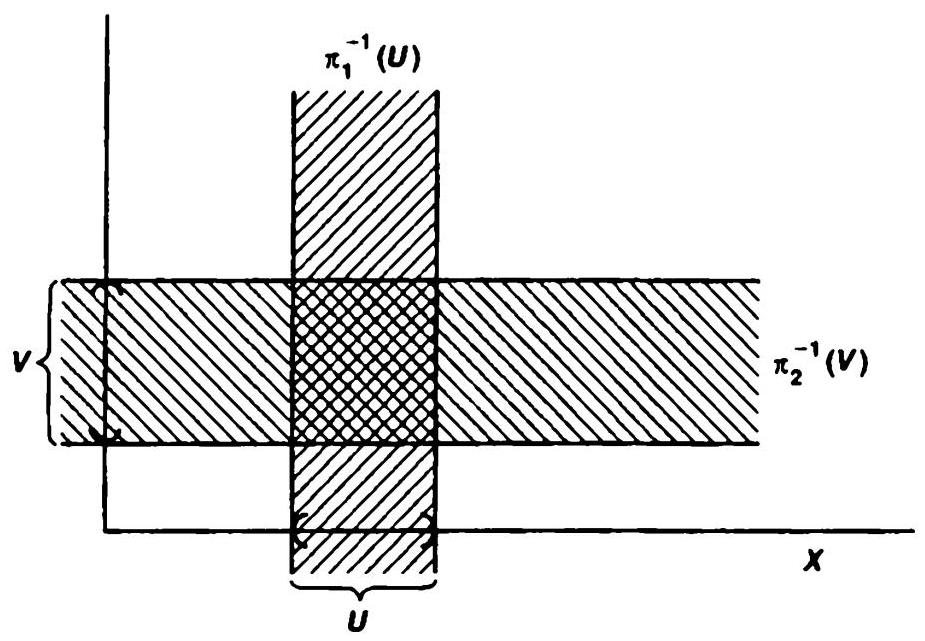
\includegraphics[width=0.8\textwidth]{images/15.2.jpg}
\end{center}
\hspace*{3em} 

Figure 15.2

\end{theorem}
\begin{proof}
Let \(\mathcal{T}\) denote the product topology on \(X \times  Y\) , let \({\mathcal{T}}^{\prime }\) be the topology generated by \(S\) . Because every element of \(S\) belongs to \(\mathcal{T}\) , so do arbitrary unions of finite intersections of elements of \(S\) . Thus \({\mathcal{T}}^{\prime } \subset  \mathcal{T}\) . On the other hand, every basis element \(U \times  V\) for the topology \(\mathcal{T}\) is a finite intersection of elements of \(S\) , since

\[
U \times  V = {\pi }_{1}^{-1}( U)  \cap  {\pi }_{2}^{-1}( V)
\]

Therefore, \(U \times  V\) belongs to \({\mathcal{T}}^{\prime }\) , so that \(\mathcal{T} \subset  {\mathcal{T}}^{\prime }\) as well
\end{proof}

\section*{§ 16 The Subspace Topology}

\index{Subspace Topology}
\begin{definition}
	Let \(X\) be a topological space with topology \(\mathcal{T}\) . If \(Y\) is a subset of \(X\) , the collection

\[
{\mathcal{T}}_{Y} = \{ Y \cap  U \mid  U \in  \mathcal{T}\}
\]

is a topology on \(Y\) , called the \index{Subspace topology}subspace topology. With this topology, \(Y\) is called a subspace of \(X\) ; its open sets consist of all intersections of open sets of \(X\) with \(Y\) .
\end{definition}

It is easy to see that \({\mathcal{T}}_{Y}\) is a topology. It contains \(\varnothing\) and \(Y\) because

\[
\varnothing  = Y \cap  \varnothing \;\text{ and }\;Y = Y \cap  X,
\]

where \(\varnothing\) and \(X\) are elements of \(\mathcal{T}\) . The fact that it is closed under finite intersections and arbitrary unions follows from the equations

\[
( {{U}_{1} \cap  Y})  \cap  \cdots  \cap  ( {{U}_{n} \cap  Y})  = ( {{U}_{1} \cap  \cdots  \cap  {U}_{n}})  \cap  Y
\]

\[
\mathop{\bigcup }\limits_{{\alpha  \in  J}}( {{U}_{\alpha } \cap  Y})  = ( {\mathop{\bigcup }\limits_{{\alpha  \in  J}}{U}_{\alpha }})  \cap  Y
\]

\begin{lemma}
	If \(\mathcal{B}\) is a basis for the topology of \(X\) then the collection

\[
{\mathcal{B}}_{Y} = \{ B \cap  Y \mid  B \in  \mathcal{B}\}
\]

is a basis for the subspace topology on \(Y\) .
\end{lemma}

\begin{proof}
Given \(U\) open in \(X\) and given \(y \in  U \cap  Y\) , we can choose an element \(B\) of \(\mathcal{B}\) such that \(y \in  B \subset  U\) . Then \(y \in  B \cap  Y \subset  U \cap  Y\) . It follows from Lemma 13.2 that \({\mathcal{B}}_{Y}\) is a basis for the subspace topology on \(Y\) .

When dealing with a space \(X\) and a subspace \(Y\) , one needs to be careful when one uses the term ``open set''. Does one mean an element of the topology of \(Y\) or an element of the topology of \(X\) ? We make the following definition : If \(Y\) is a subspace of \(X\) , we say that a set \(U\) is open in \(Y\) (or open relative to \(Y\) ) if it belongs to the topology of \(Y\) ; this implies in particular that it is a subset of \(Y\) . We say that \(U\) is open in \(X\) if it belongs to the topology of \(X\)

There is a special situation in which every set open in \(Y\) is also open in \(\mathbf{X}\) .
\end{proof}

\begin{lemma}
	Let \(Y\) be a subspace of \(X\) . If \(U\) is open in \(Y\) and \(Y\) is open in \(X\) , then \(U\) is open in \(X\) .
\end{lemma}

\begin{proof}
Since \(U\) is open in \(Y,U = Y \cap  V\) for some set \(V\) open in \(X\) . Since \(Y\) and \(V\) are both open in \(X\) , so is \(Y \cap  V\)

Now let us explore the relation between the subspace topology and the order and product topologies For product topologies, the result is what one might expect; for order topologies, it is not.
\end{proof}

\begin{theorem}
	If \(A\) is a subspace of \(X\) and \(B\) is a subspace of \(Y\) , then the product topology on \(A \times  B\) is the same as the topology \(A \times  B\) inherits as a subspace of \(X \times  Y\) .

\end{theorem}
\begin{proof}
The set \(U \times  V\) is the general basis element for \(X \times  Y\) , where \(U\) is open in \(X\) and \(V\) is open in \(Y\) . Therefore, \(( {U \times  V})  \cap  ( {A \times  B})\) is the general basis element for the subspace topology on \(A \times  B\) . Now

\[
( {U \times  V})  \cap  ( {A \times  B})  = ( {U \cap  A})  \times  ( {V \cap  B}) .
\]

Since \(U \cap  A\) and \(V \cap  B\) are the general open sets for the subspace topologies on \(A\) and \(B\) , respectively, the set \(( {U \cap  A})  \times  ( {V \cap  B})\) is the general basis element for the product topology on \(A \times  B\) .

The conclusion we draw is that the bases for the subspace topology on \(A \times  B\) and for the product topology on \(A \times  B\) are the same. Hence the topologies are the same. ∎

Now let \(X\) be an ordered set in the order topology, and let \(Y\) be a subset of \(X\) . The order relation on \(X\) , when restricted to \(Y\) , makes \(Y\) into an ordered set. However, the resulting order topology on \(Y\) need not be the same as the topology that \(Y\) inherits as a subspace of \(X\) . We give one example where the subspace and order topologies on \(Y\) agree, and two examples where they do not.
\end{proof}

\begin{centeredblock}
\begin{example}
	Consider the subset \(Y = [  {0,1}]\) of the real line \(\mathbb{R}\) , in the subspace topology. The subspace topology has as basis all sets of the form \(( {a,b})  \cap  Y\) , where(a, b)is an open interval in \(\mathbb{R}\) Such a set is of one of the following types.

\[
( {a,b})  \cap  Y = \{ \begin{array}{ll} ( {a,b}) & \text{ if }a\text{ and }b\text{ are in }Y, \\  \lbrack 0,b) & \text{ if only }b\text{ is in }Y, \\  ( {a,1}) & \text{ if only }a\text{ is in }Y, \\  Y\text{ or }\varnothing & \text{ if neither }a\text{ nor }b\text{ is in }Y. \end{array}.
\]

By definition, each of these sets is open in \(Y\) But sets of the second and third types are not open in the larger space \(\mathbb{R}\) .

Note that these sets form a basis for the order topology on \(Y\) Thus, we see that in the case of the set \(Y = [  {0,1}]\) , its subspace topology (as a subspace of \(\mathbb{R}\) ) and its order topology are the same.
\end{example}
\end{centeredblock}

\begin{centeredblock}
\begin{example}
	Let \(Y\) be the subset \(\lbrack 0,1) \cup  \{ 2\}\) of \(\mathbb{R}\) . In the subspace topology on \(Y\) the one-point set \(\{ 2\}\) is open, because it is the intersection of the open set \(( {\frac{3}{2},\frac{5}{2}})\) with \(Y\) But in the order topology on \(Y\) , the set \(\{ 2\}\) is not open. Any basis element for the order topology on \(Y\) that contains 2 is of the form

\[
\{ x \mid  x \in  Y\text{ and }a < x \leq  2\}
\]

for some \(a \in  Y\) , such a set necessarily contains points of \(Y\) less than 2
\end{example}
\end{centeredblock}

\begin{centeredblock}
\begin{example}
	Let \(I = [  {0,1}]\) The dictionary order on \(I \times  I\) is just the restriction to \(I \times  I\) of the dictionary order on the plane \(\mathbb{R} \times  \mathbb{R}\) . However, the dictionary order topology on \(I \times  I\) is not the same as the subspace topology on \(I \times  I\) obtained from the dictionary order topology on \(\mathbb{R} \times  {\mathbb{R}}^{1}\) For example, the set \(\{ 1/2\}  \times  (1/2,1\rbrack\) is open in \(I \times  I\) in the subspace topology, but not in the order topology, as you can check. See Figure 16.1.
\end{example}
\end{centeredblock}

The set \(I \times  I\) in the dictionary order topology will be called the ordered \index{Square metric (see also )} square, and denoted by \(\index{I@\({I}_{o}^{2}\)} {I}_{o}^{2}\) .

The anomaly illustrated in Examples 2 and 3 does not occur for intervals or rays in an ordered set \(X\) . This we now prove.

Given an ordered set \(X\) , let us say that a subset \(Y\) of \(X\) is \index{Convex set: in an ordered set} convex in \(X\) if for each pair of points \(a < b\) of \(Y\) , the entire interval(a, b)of points of \(X\) lies in \(Y\) . Note that intervals and rays in \(X\) are convex in \(X\) .

\begin{center}
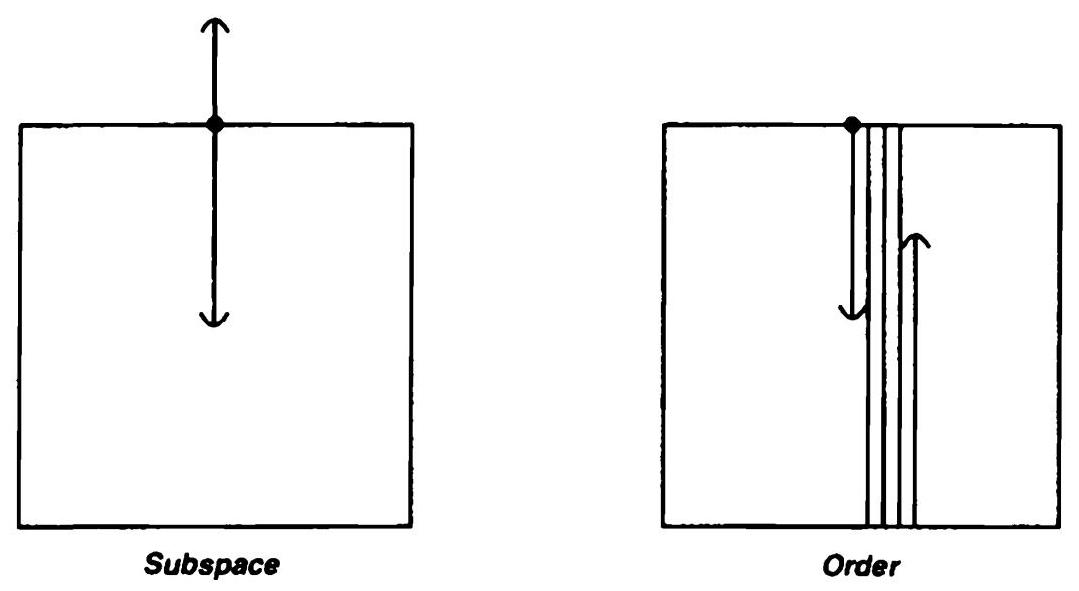
\includegraphics[width=1.0\textwidth]{images/16.1.jpg}
\end{center}
\hspace*{3em} 

Figure 16.1

\begin{theorem}
	Let \(X\) be an ordered set in the order topology; let \(Y\) be a subset of \(X\) that is convex in \(X\) Then the order topology on \(Y\) is the same as the topology \(Y\) inherits as a subspace of \(X\) .

\end{theorem}
\begin{proof}
Consider the ray \(( {a, + \infty })\) in \(X\) . What is its intersection with \(Y\) ? If \(a \in  Y\) , then

\[
( {a, + \infty })  \cap  Y = \{ x \mid  x \in  Y\text{ and }x > a\} ;
\]

this is an open ray of the ordered set \(Y\) . If \(a \notin  Y\) , then \(a\) is either a lower bound on \(Y\) or an upper bound on \(Y\) , since \(Y\) is convex. In the former case, the set \(( {a, + \infty })  \cap  Y\) equals all of \(Y\) ; in the latter case, it is empty.

A similar remark shows that the intersection of the ray \(( {-\infty ,a})\) with \(Y\) is either an open ray of \(Y\) , or \(Y\) itself, or empty. Since the sets \(( {a, + \infty })  \cap  Y\) and \(( {-\infty ,a})  \cap  Y\) form a subbasis for the subspace topology on \(Y\) , and since each is open in the order topology, the order topology contains the subspace topology.

To prove the reverse, note that any open ray of \(Y\) equals the intersection of an open ray of \(X\) with \(Y\) , so it is open in the subspace topology on \(Y\) . Since the open rays of \(Y\) are a subbasis for the order topology on \(Y\) , this topology is contained in the subspace topology.

To avoid ambiguity, let us agree that whenever \(X\) is an ordered set in the order topology and \(Y\) is a subset of \(X\) , we shall assume that \(Y\) is given the subspace topology unless we specifically state otherwise. If \(Y\) is convex in \(X\) , this is the same as the order topology on \(Y\) , otherwise, it may not be.
\end{proof}

\section*{Exercises}
\begin{enumerate}[itemsep=0.4em, parsep=0pt, topsep=0pt, partopsep=0pt, leftmargin=*, label=\arabic*., ref=\arabic*]
\item Show that if \(Y\) is a subspace of \(X\) , and \(A\) is a subset of \(Y\) , then the topology \(A\) inherits as a subspace of \(Y\) is the same as the topology it inherits as a subspace of \(X\) .
\item If \(\mathcal{T}\) and \({\mathcal{T}}^{\prime }\) are topologies on \(X\) and \({\mathcal{T}}^{\prime }\) is strictly finer than \(\mathcal{T}\) , what can you say about the corresponding subspace topologies on the subset \(Y\) of \(X\) ?
\item Consider the set \(Y = \{  - 1,1\}\) as a subspace of \(\mathbb{R}\) . Which of the following sets are open in \(Y\) ? Which are open in \(\mathbb{R}\) ? \[ A = \{  {x| {\frac{1}{2} < }| x \mid   < 1}\}  , \] \[ B = \{  {x| {\frac{1}{2} < }| x \mid   \leq  1}\}  , \] \[ C = \{  {x| {\frac{1}{2} \leq  }| x \mid   < 1}\}  , \] \[ D = \{  {x| {\frac{1}{2} \leq  }| x \mid   \leq  1}\}  \text{ , } \] \[ E = \{  {x| {0 < }| x \mid   < 1\text{ and }1/x \notin  {\mathbb{Z}}_{ + }}\}  . \]
\item A map \(f : X \rightarrow  Y\) is said to be an \index{open map} if for every open set \(U\) of \(X\) , the set \(f( U)\) is open in \(Y\) . Show that \({\pi }_{1} : X \times  Y \rightarrow  X\) and \({\pi }_{2} : X \times  Y \rightarrow  Y\) are \index{Open map}open maps.
\item Let \(X\) and \({X}^{\prime }\) denote a single set in the topologies \(\mathcal{T}\) and \({\mathcal{T}}^{\prime }\) , respectively; let \(Y\) and \({Y}^{\prime }\) denote a single set in the topologies \(\mathcal{U}\) and \({\mathcal{U}}^{\prime }\) , respectively. Assume these sets are nonempty.
  \begin{enumerate}[itemsep=0.2em, parsep=0pt, topsep=0pt, partopsep=0pt, leftmargin=*, label=(\alph*), align=left]
  \item Show that if \({\mathcal{T}}^{\prime } \supset  \mathcal{T}\) and \({\mathcal{U}}^{\prime } \supset  \mathcal{U}\) , then the product topology on \({X}^{\prime } \times  {Y}^{\prime }\) is finer than the product topology on \(X \times  Y\) .
  \item Does the converse of (a) hold? Justify your answer.
  \end{enumerate}
\item Show that the countable collection \[ \{ ( {a,b})  \times  ( {\mathrm{c},d})  \mid  a < b\text{ and }\mathrm{c} < d\text{ , and }a,b,\mathrm{c},d\text{ are rational }\} \] is a basis for \({\mathbb{R}}^{2}\) .
\item Let \(X\) be an ordered set. If \(Y\) is a proper subset of \(X\) that is convex in \(X\) , does it follow that \(Y\) is an interval or a ray in \({X}^{\gamma }\)
\item If \(L\) is a straight line in the plane, describe the topology \(L\) inherits as a subspace of \({\mathbb{R}}_{\ell } \times  \mathbb{R}\) and as a subspace of \({\mathbb{R}}_{\ell } \times  {\mathbb{R}}_{\ell }\) . In each case it is a familiar topology.
\item Show that the dictionary order topology on the set \(\mathbb{R} \times  \mathbb{R}\) is the same as the product topology \({\mathbb{R}}_{d} \times  \mathbb{R}\) , where \({\mathbb{R}}_{d}\) denotes \(\mathbb{R}\) in the discrete topology. Compare this topology with the standard topology on \({\mathbb{R}}^{2}\) .
\item Let \(I = [  {0,1}]\) . Compare the product topology on \(I \times  I\) , the dictionary order topology on \(I \times  I\) , and the topology \(I \times  I\) inherits as a subspace of \(\mathbb{R} \times  \mathbb{R}\) in the dictionary order topology.
\end{enumerate}
\section*{§ 17 Closed Sets and Limit Points}

Now that we have a few examples at hand, we can introduce some of the basic concepts associated with topological spaces. In this section, we treat the notions of closed set, \index{Closure (cont.)} closure of a set, and limit point. These lead naturally to consideration of a certain axiom for topological spaces called the Hausdorff axiom.

\section*{Closed Sets}

A subset \(A\) of a topological space \(X\) is said to be closed if the set \(X - A\) is open.

\begin{centeredblock}
\begin{example}
	The subset \([  {a,b}]\) of \(\mathbb{R}\) is closed because its complement

\[
\mathbb{R} - [  {a,b}]   = ( {-\infty ,a})  \cup  ( {b, + \infty }) ,
\]

is open. Similarly, \(\lbrack a, + \infty )\) is closed, because its complement \(( {-\infty ,a})\) is open. These facts justify our use of the terms ``\index{Closed interval}closed interval'' and ``\index{Closed ray}closed ray'' The subset \(\lbrack a,b)\) of \(\mathbb{R}\) is neither open nor closed.
\end{example}
\end{centeredblock}

\begin{centeredblock}
\begin{example}
	In the plane \({\mathbb{R}}^{2}\) , the set

\[
\{ x \times  y \mid  x \geq  0\text{ and }y \geq  0\}
\]

is closed, because its complement is the union of the two sets

\[
( {-\infty ,0})  \times  \mathbb{R}\;\text{ and }\;\mathbb{R} \times  ( {-\infty ,0}) ,
\]

each of which is a product of open sets of \(\mathbb{R}\) and is, therefore, open in \({\mathbb{R}}^{2}\)
\end{example}
\end{centeredblock}

\begin{centeredblock}
\begin{example}
	In the finite complement topology on a set \(X\) , the closed sets consist of \(X\) itself and all finute subsets of \(X\)
\end{example}
\end{centeredblock}

\begin{centeredblock}
\begin{example}
	In the discrete topology on the set \(X\) , every set is open, it follows that every set is closed as well.
\end{example}
\end{centeredblock}

\begin{centeredblock}
\begin{example}
	Consider the following subset of the real line:

\[
Y = [  {0,1}]   \cup  ( {2,3}) \text{ , }
\]

in the subspace topology. In this space, the set \([  {0,1}]\) is open, since it is the intersection of the open set \(( {-\frac{1}{2},\frac{3}{2}})\) of \(\mathbb{R}\) with \(Y\) Similarly,(2,3)is open as a subset of \(Y\) ; it is even open as a subset of \(\mathbb{R}\) . Since \([  {0,1}]\) and(2,3)are complements in \(Y\) of each other, we conclude that both \([  {0,1}]\) and(2,3)are closed as subsets of \(Y\)
\end{example}
\end{centeredblock}

These examples suggest that an answer to the mathematician's riddle: ``How is a set different from a door?'' should be: ``A door must be either open or closed, and cannot be both, while a set can be open, or closed, or both, or neither!''

The collection of closed subsets of a space \(X\) has properties similar to those satisfied by the collection of open subsets of \(X\) :

\begin{theorem}
	Let \(X\) be a topological space. Then the following conditions hold:

(1) \(\varnothing\) and \(X\) are closed.

(2) Arbitrary intersections of closed sets are closed.

(3) Finite unions of closed sets are closed.

\end{theorem}
\begin{proof}
(1) \(\varnothing\) and \(X\) are closed because they are the complements of the open sets \(X\) and \(\varnothing\) , respectively.

(2) Given a collection of closed sets \({\{  {A}_{\alpha }\}  }_{\alpha  \in  J}\) , we apply DeMorgan's law,

\[
X - \mathop{\bigcap }\limits_{{\alpha  \in  J}}{A}_{\alpha } = \mathop{\bigcup }\limits_{{\alpha  \in  J}}( {X - {A}_{\alpha }})
\]

Since the sets \(X - {A}_{\alpha }\) are open by definition, the right side of this equation represents an arbitrary union of open sets, and is thus open. Therefore, \(\cap  {A}_{\alpha }\) is closed.

(3) Similarly, if \({A}_{i}\) is closed for \(i = 1,\ldots ,n\) , consider the equation

\[
X - \mathop{\bigcup }\limits_{{i = 1}}^{n}{A}_{i} = \mathop{\bigcap }\limits_{{i = 1}}^{n}( {X - {A}_{i}})
\]

The set on the right side of this equation is a finite intersection of open sets and is therefore open. Hence \(\bigcup {A}_{i}\) is closed.

Instead of using open sets, one could just as well specify a topology on a space by giving a collection of sets (to be called ``\index{Closed set}closed sets'') satisfying the three properties of this theorem. One could then define open sets as the complements of closed sets and proceed just as before. This procedure has no particular advantage over the one we have adopted, and most mathematicians prefer to use open sets to define topologies.

Now when dealing with subspaces, one needs to be careful in using the term ``closed set.'' If \(Y\) is a subspace of \(X\) , we say that a set \(A\) is closed in \(Y\) if \(A\) is a subset of \(Y\) and if \(A\) is closed in the subspace topology of \(Y\) (that is, if \(Y - A\) is open in \(Y\) ). We have the following theorem:
\end{proof}

\begin{theorem}
	Let \(Y\) be a subspace of \(X\) . Then a set \(A\) is closed in \(Y\) if and only if it equals the intersection of a closed set of \(X\) with \(Y\) .

\end{theorem}
\begin{proof}
Assume that \(A = C \cap  Y\) , where \(C\) is closed in \(X\) . (See Figure 17.1.) Then \(X - C\) is open in \(X\) , so that \(( {X - C})  \cap  Y\) is open in \(Y\) , by definition of the subspace topology. But \(( {X - C})  \cap  Y = Y - A\) . Hence \(Y - A\) is open in \(Y\) , so that \(A\) is closed in \(Y\) . Conversely, assume that \(A\) is closed in \(Y\) . (See Figure 17.2.) Then \(Y - A\) is open in \(Y\) , so that by definition it equals the intersection of an open set \(U\) of \(X\) with \(Y\) The set \(X - U\) is closed in \(X\) , and \(A = Y \cap  ( {X - U})\) , so that \(A\) equals the intersection of a closed set of \(X\) with \(Y\) , as desired.

A set \(A\) that is closed in the subspace \(Y\) may or may not be closed in the larger space \(X\) . As was the case with open sets, there is a criterion for \(A\) to be closed in \(X\) ; we leave the proof to you.

\begin{center}
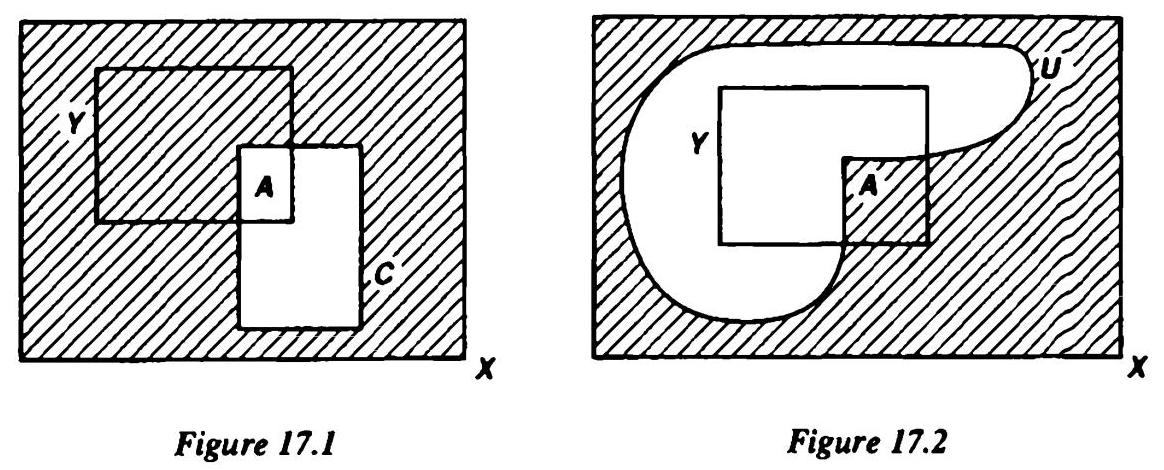
\includegraphics[width=1.0\textwidth]{images/17.1.jpg}
\end{center}
\hspace*{3em} 
\end{proof}

\begin{theorem}
	Let \(Y\) be a subspace of \(X\) . If \(A\) is closed in \(Y\) and \(Y\) is closed in \(X\) , then \(A\) is closed in \(X\) .

\end{theorem}
\section*{Closure and Interior of a Set}

Given a subset \(A\) of a topological space \(X\) , the interior of \(A\) is defined as the union of all open sets contained in \(A\) , and the closure of \(A\) is defined as the intersection of all closed sets containing \(A\) .

The interior of \(A\) is denoted by Int \(A\) and the closure of \(A\) is denoted by \(\mathrm{{Cl}}A\) or by \(\index{A@\(\bar{A}\)}\) . Obviously Int \(A\) is an open set and \(\bar{A}\) is a closed set; furthermore,

\[
\operatorname{Int}A \subset  A \subset  \bar{A}.
\]

If \(A\) is open, \(A = \operatorname{Int}A\) ; while if \(A\) is closed, \(A = \bar{A}\) .

We shall not make much use of the interior of a set, but the \index{Closure}closure of a set will be quite important.

When dealing with a topological space \(X\) and a subspace \(Y\) , one needs to exercise care in taking closures of sets If \(A\) is a subset of \(Y\) , the closure of \(A\) in \(Y\) and the closure of \(A\) in \(X\) will in general be different In such a situation, we reserve the notation \(\bar{A}\) to stand for the closure of \(A\) in \(X\) . The closure of \(A\) in \(Y\) can be expressed in terms of \(\bar{A}\) , as the following theorem shows:

\begin{theorem}
	Let \(Y\) be a subspace of \(X\) , let \(A\) be a subset of \(Y\) , let \(\bar{A}\) denote the closure of \(A\) in \(X\) . Then the closure of \(A\) in \(Y\) equals \(\bar{A} \cap  Y\) .

\end{theorem}
\begin{proof}
Let \(B\) denote the closure of \(A\) in \(Y\) . The set \(\bar{A}\) is closed in \(X\) , so \(\bar{A} \cap  Y\) is closed in \(Y\) by Theorem 17.2. Since \(\bar{A} \cap  Y\) contains \(A\) , and since by definition \(B\) equals the intersection of all closed subsets of \(Y\) containing \(A\) , we must have \(B \subset  ( {\bar{A} \cap  Y})\) .

On the other hand, we know that \(B\) is closed in \(Y\) . Hence by Theorem 17.2, \(B = C \cap  Y\) for some set \(C\) closed in \(X\) . Then \(C\) is a closed set of \(X\) containing \(A\) ; because \(\bar{A}\) is the intersection of all such closed sets, we conclude that \(\bar{A} \subset  C\) . Then \(( {\bar{A} \cap  Y})  \subset  ( {C \cap  Y})  = B.\)

The definition of the closure of a set does not give us a convenient way for actually finding the closures of specific sets, since the collection of all closed sets in \(X\) , like the collection of all open sets, is usually much too big to work with. Another way of describing the closure of a set, useful because it involves only a basis for the topology of \(X\) , is given in the following theorem.

First let us introduce some convenient terminology. We shall say that a set \(A\) intersects a set \(B\) if the intersection \(A \cap  B\) is not empty.
\end{proof}

\begin{theorem}
	Let \(A\) be a subset of the topological space \(X\) .

(a) Then \(x \in  \bar{A}\) if and only if every open set \(U\) containing \(x\) intersects \(A\) .

(b) Supposing the topology of \(X\) is given by a basis, then \(x \in  \bar{A}\) if and only if every basis element \(B\) containing \(x\) intersects \(A\) .

\end{theorem}
\begin{proof}
Consider the statement in (a). It is a statement of the form \(P \Leftrightarrow  Q\) . Let us transform each implication to its contrapositive, thereby obtaining the logically equivalent statement (not \(P\) ) \(\Leftrightarrow\) (not \(Q\) ). Written out, it is the following.

\(x \notin  \bar{A} \Leftrightarrow\) there exists an open set \(U\) containing \(x\) that does not intersect \(A\) .

In this form, our theorem is easy to prove. If \(x\) is not in \(\bar{A}\) , the set \(U = X - \bar{A}\) is an open set containing \(x\) that does not intersect \(A\) , as desired Conversely, if there exists an open set \(U\) containing \(x\) which does not intersect \(A\) , then \(X - U\) is a closed set containing \(A\) By definition of the closure \(\bar{A}\) , the set \(X - U\) must contain \(\bar{A}\) , therefore, \(x\) cannot be in \(\bar{A}\) .

Statement (b) follows readily If every open set containing \(x\) intersects \(A\) , so does every basis element \(B\) containing \(x\) , because \(B\) is an open set. Conversely, if every basis element containing \(x\) intersects \(A\) , so does every open set \(U\) containing \(x\) , because \(U\) contains a basis element that contains \(x\) .

Mathematicians often use some special terminology here. They shorten the statement `` \(U\) is an open set containing \(x\) `` to the phrase

\[
\text{ " }U\text{ is a neighborhood of }x\text{ ." }
\]

Using this terminology, one can write the first half of the preceding theorem as follows:

If \(A\) is a subset of the topological space \(X\) , then \(x \in  \widehat{A}\) if and only if every \index{neighborhood} of \(x\) intersects \(A\) .
\end{proof}

\begin{centeredblock}
\begin{example}
	Let \(X\) be the real line \(\mathbb{R}\) . If \(A = (0,1\rbrack\) , then \(\bar{A} = [  {0,1}]\) , for every \index{Neighborhood}neighborhood of 0 intersects \(A\) , while every point outside \([  {0,1}]\) has a neighborhood disjoint from \(A\) Similar arguments apply to the following subsets of \(X\)

If \(B = \{  {1/n \mid  n \in  {\mathbb{Z}}_{ + }}\}\) , then \(\bar{B} = \{ 0\}  \cup  B\) If \(C = \{ 0\}  \cup  ( {1,2})\) , then \(\bar{C} = \{ 0\}  \cup  [  {1,2}]\) If \(\mathbb{Q}\) is the set of rational numbers, then \(\widehat{\mathbb{Q}} = \mathbb{R}\) If \({\mathbb{Z}}_{ + }\) is the set of positive integers, then \({\overline{\mathbb{Z}}}_{ + } = {\mathbb{Z}}_{ + }\) . If \({\mathbb{R}}_{ + }\) is the set of positive reals, then the closure of \({\mathbb{R}}_{ + }\) is the set \({\mathbb{R}}_{ + } \cup  \{ 0\}\) . (This is the reason we introduced the notation \({\overline{\mathbb{R}}}_{ + }\) for the set \({\mathbb{R}}_{ + } \cup  \{ 0\}\) , back in \(\$ 2\) )
\end{example}
\end{centeredblock}

\begin{centeredblock}
\begin{example}
	Consider the subspace \(Y = (0,1\rbrack\) of the real line \(\mathbb{R}\) . The set \(A = ( {0,\frac{1}{2}})\) is a subset of \(Y\) , its closure in \(\mathbb{R}\) is the set \([  {0,\frac{1}{2}}]\) , and its closure in \(Y\) is the set \([  {0,\frac{1}{2}}]   \cap  Y =\)  \(( {0,\frac{1}{2}}]\)
\end{example}
\end{centeredblock}

Some mathematicians use the term ``neighborhood'' differently. They say that \(A\) is a neighborhood of \(x\) if \(A\) merely contains an open set containing \(x\) . We shall not follow this practice.

\section*{Limit Points}

There is yet another way of describing the closure of a set, a way that involves the important concept of limit point, which we consider now.

If \(A\) is a subset of the topological space \(X\) and if \(x\) is a point of \(X\) , we say that \(x\) is a limit point (or ``cluster point,'' or ``point of accumulation'') of \(A\) if every neighborhood of \(x\) intersects \(A\) in some point other than \(x\) itself. Said differently, \(x\) is a limit point of \(A\) if it belongs to the closure of \(A - \{ x\}\) The point \(x\) may lie in \(A\) or not; for this definition it does not matter.

\begin{centeredblock}
\begin{example}
	Consider the real line \(\mathbb{R}\) . If \(A = (0,1\rbrack\) , then the point 0 is a limit point of \(A\) and so is the point \(\frac{1}{2}\) . In fact, every point of the interval \([  {0,1}]\) is a \index{Limit point}limit point of \(A\) , but no other point of \(\mathbb{R}\) is a limit point of \(A\)

If \(B = \{  {1/n \mid  n \in  {\mathbb{Z}}_{ + }}\}\) , then 0 is the only limit point of \(B\) . Every other point \(x\) of \(\mathbb{R}\) has a neighborhood that either does not intersect \(B\) at all, or it intersects \(B\) only in the point \(x\) itself. If \(C = \{ 0\}  \cup  ( {1,2})\) , then the limit points of \(C\) are the points of the interval \([  {1,2}]\) . If \(\mathbb{Q}\) is the set of rational numbers, every point of \(\mathbb{R}\) is a limit point of \(\mathbb{Q}\) . If \({\mathbb{Z}}_{ + }\) is the set of positive integers, no point of \(\mathbb{R}\) is a limit point of \({\mathbb{Z}}_{ + }\) . If \({\mathbb{R}}_{ + }\) is the set of positive reals, then every point of \(\{ 0\}  \cup  {\mathbb{R}}_{ + }\) is a limit point of \({\mathbb{R}}_{ + }\)
\end{example}
\end{centeredblock}

\index{Comparison test for infinite series} Comparison of Examples 6 and 8 suggests a relationship between the closure of a set and the limit points of a set. That relationship is given in the following theorem:

\begin{theorem}
	Let \(A\) be a subset of the topological space \(X\) , let \({A}^{\prime }\) be the set of all limit points of \(A\) . Then

\[
\bar{A} = A \cup  {A}^{\prime }.
\]

\end{theorem}
\begin{proof}
If \(x\) is in \({A}^{\prime }\) , every neighborhood of \(x\) intersects \(A\) (in a point different from \(x\) ). Therefore, by Theorem 17.5, \(x\) belongs to \(\bar{A}\) Hence \({A}^{\prime } \subset  \bar{A}\) . Since by definition \(A \subset  \bar{A}\) , it follows that \(A \cup  {A}^{\prime } \subset  \bar{A}\) .

To demonstrate the reverse inclusion, we let \(x\) be a point of \(\bar{A}\) and show that \(x \in  A \cup  {A}^{\prime }\) . If \(x\) happens to lie in \(A\) , it is trivial that \(x \in  A \cup  {A}^{\prime }\) ; suppose that \(x\) does not lie in \(A\) . Since \(x \in  \bar{A}\) , we know that every neighborhood \(U\) of \(x\) intersects \(A\) ; because \(x \notin  A\) , the set \(U\) must intersect \(A\) in a point different from \(x\) . Then \(x \in  {A}^{\prime }\) , so that \(x \in  A \cup  {A}^{\prime }\) , as desired.
\end{proof}

\begin{corollary}
	A subset of a topological space is closed if and only if it contains all its limit points.
\end{corollary}

Proof The set \(A\) is closed if and only if \(A = \bar{A}\) , and the latter holds if and only if \({A}^{\prime } \subset  A\) .

\section*{Hausdorff Spaces}

One's experience with open and closed sets and limit points in the real line and the plane can be misleading when one considers more general topological spaces. For example, in the spaces \(\mathbb{R}\) and \({\mathbb{R}}^{2}\) , each one-point set \(\{  {x}_{0}\}\) is closed. This fact is easily proved; every point different from \({x}_{0}\) has a neighborhood not intersecting \(\{  {x}_{0}\}\) , so that \(\{  {x}_{0}\}\) is its own closure. But this fact is not true for arbitrary topological spaces. Consider the topology on the three-point set \(\{ a,b,c\}\) indicated in Figure 17.3. In this space, the one-point set \(\{ b\}\) is not closed, for its complement is not open.

\begin{center}
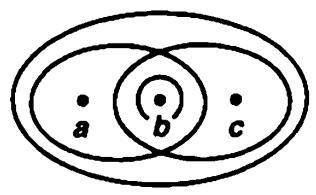
\includegraphics[width=0.2\textwidth]{images/17.3.jpg}
\end{center}
\hspace*{3em} 

Figure 17.3

Similarly, one's experience with the properties of \index{convergent sequence} in \(\mathbb{R}\) and \({\mathbb{R}}^{2}\) can be misleading when one deals with more general topological spaces. In an arbitrary topological space, one says that a sequence \({x}_{1},{x}_{2},\ldots\) of points of the space \(X\) converges to the point \(x\) of \(X\) provided that, corresponding to each neighborhood \(U\) of \(x\) , there is a positive integer \(N\) such that \({x}_{n} \in  U\) for all \(n \geq  N\) . In \(\mathbb{R}\) and \({\mathbb{R}}^{2}\) , a sequence cannot converge to more than one point, but in an arbitrary space, it can. In the space indicated in Figure 17.3, for example, the sequence defined by setting \({x}_{n} = b\) for all \(n\) converges not only to the point \(b\) , but also to the point \(a\) and to the point \(c\) !

Topologies in which one-point sets are not closed, or in which sequences can converge to more than one point, are considered by many mathematicians to be somewhat strange. They are not really very interesting, for they seldom occur in other branches of mathematics And the theorems that one can prove about topological spaces are rather limited if such examples are allowed. Therefore, one often imposes an additional condition that will rule out examples like this one, bringing the class of spaces under consideration closer to those to which one's geo\index{Metric}metric intuition applies. The condition was suggested by the mathematician Felix Hausdorff, so mathematicians have come to call it by his name.

\begin{definition}
	A topological space \(X\) is called a \index{Hausdorff space} if for each pair \({x}_{1},{x}_{2}\) of distinct points of \(X\) , there exist neighborhoods \({U}_{1}\) , and \({U}_{2}\) of \({x}_{1}\) and \({x}_{2}\) , respectively, that are disjoint.
\end{definition}

\section*{Theorem 17.8. Every finite point set in a Hausdorff space \(X\) is closed.}

\begin{proof}
It suffices to show that every one-point set \(\{  {x}_{0}\}\) is closed. If \(x\) is a point of \(X\) different from \({x}_{0}\) , then \(x\) and \({x}_{0}\) have disjoint neighborhoods \(U\) and \(V\) , respectively. Since \(U\) does not intersect \(\{  {x}_{0}\}\) , the point \(x\) cannot belong to the closure of the set \(\{  {x}_{0}\}\) . As a result, the closure of the set \(\{  {x}_{0}\}\) is \(\{  {x}_{0}\}\) itself, so that it is closed.

The condition that finite point sets be closed is in fact weaker than the \index{Hausdorff condition} For example, the real line \(\mathbb{R}\) in the finite complement topology is not a Hausdorff space, but it is a space in which finite point sets are closed The condition that finite point sets be closed has been given a name of its own: it is called the \({T}_{1}{ax}\) - iom. (We shall explain the reason for this strange terminology in Chapter 4.) The \({T}_{1}\) axiom will appear in this book in a few exercises, and in just one theorem, which is the following:
\end{proof}

\begin{theorem}
	Let \(X\) be a space satisfying the \({T}_{1}\) axiom; let \(A\) be a subset of \(X\) . Then the point \(x\) is a limit point of \(A\) if and only if every neighborhood of \(x\) contains infinitely many points of \(A\) .

\end{theorem}
\begin{proof}
If every neighborhood of \(x\) intersects \(A\) in infinitely many points, it certainly intersects \(A\) in some point other than \(x\) itself, so that \(x\) is a limit point of \(A\)

Conversely, suppose that \(x\) is a limit point of \(A\) , and suppose some neighborhood \(U\) of \(x\) intersects \(A\) in only finitely many points. Then \(U\) also intersects \(A - \{ x\}\) in finitely many points; let \(\{  {{x}_{1},\ldots ,{x}_{m}}\}\) be the points of \(U \cap  ( {A-\{ x\} })\) . The set \(X - \{  {{x}_{1},\ldots ,{x}_{m}}\}\) is an open set of \(X\) , since the finite point set \(\{  {{x}_{1},\ldots ,{x}_{m}}\}\) is closed; then

\[
U \cap  ( {X - \{  {{x}_{1},\ldots ,{x}_{m}}\}  })
\]

is a neighborhood of \(x\) that intersects the set \(A - \{ x\}\) not at all. This contradicts the assumption that \(x\) is a limit point of \(A\) .

One reason for our lack of interest in the \({T}_{1}\) axiom is the fact that many of the interesting theorems of topology require not just that axiom, but the full strength of the Hausdorff axiom. Furthermore, most of the spaces that are important to mathematicians are \index{Hausdorff space}Hausdorff spaces. The following two theorems give some substance to these remarks.
\end{proof}

\begin{theorem}
	If \(X\) is a Hausdorff space, then a sequence of points of \(X\) converges to at most one point of \(X\)

\end{theorem}
Proof Suppose that \({x}_{n}\) is a sequence of points of \(X\) that converges to \(x\) If \(y \neq  x\) , let \(U\) and \(V\) be disjoint neighborhoods of \(x\) and \(y\) , respectively. Since \(U\) contains \({x}_{n}\) for all but finitely many values of \(n\) , the set \(V\) cannot Therefore, \({x}_{n}\) cannot converge to y.

If the sequence \({x}_{n}\) of points of the Hausdorff space \(X\) converges to the point \(x\) of \(X\) , we often write \({x}_{n} \rightarrow  x\) , and we say that \(x\) is the limit of the sequence \({x}_{n}\) .

The proof of the following result is left to the exercises.

\begin{theorem}
	Every simply ordered set is a Hausdorff space in the order topology. The product of two Hausdorff spaces is a Hausdorff space. A subspace of a Hausdorff space is a Hausdorff space.

The Hausdorff condition is generally considered to be a very mild extra condition to impose on a topological space. Indeed, in a first course in topology some mathematicians go so far as to impose this condition at the outset, refusing to consider spaces that are not Hausdorff spaces. We shall not go this far, but we shall certainly assume the Hausdorff condition whenever it is needed in a proof without having any qualms about limiting seriously the range of applications of the results.

The Hausdorff condition is one of a number of extra conditions one can impose on a topological space. Each time one imposes such a condition, one can prove stronger theorems, but one limits the class of spaces to which the theorems apply. Much of the research that has been done in topology since its beginnings has centered on the problem of finding conditions that will be strong enough to enable one to prove interesting theorems about spaces satisfying those conditions, and yet not so strong that they limit severely the range of applications of the results.

We shall study a number of such conditions in the next two chapters. The Hausdorff condition and the \({T}_{1}\) axiom are but two of a collection of conditions similar to one another that are called collectively the separation axioms. Other conditions include the countability axioms, and various compactness and connectedness conditions. Some of these are quite stringent requirements, as you will see.

\end{theorem}
\section*{Exercises}
\begin{enumerate}[itemsep=0.4em, parsep=0pt, topsep=0pt, partopsep=0pt, leftmargin=*, label=\arabic*., ref=\arabic*]
\item Let \(\mathcal{C}\) be a collection of subsets of the set \(X\) . Suppose that \(\varnothing\) and \(X\) are in \(\mathcal{C}\) , and that finite unions and arbitrary intersections of elements of \(\mathcal{C}\) are in \(\mathcal{C}\) . Show that the collection \[ T = \{ X - C \mid  C \in  \mathcal{C}\} \] is a topology on \(X\) .
\item Show that if \(A\) is closed in \(Y\) and \(Y\) is closed in \(X\) , then \(A\) is closed in \(X\) .
\item Show that if \(A\) is closed in \(X\) and \(B\) is closed in \(Y\) , then \(A \times  B\) is closed in \(X \times  Y\) .
\item Show that if \(U\) is open in \(X\) and \(A\) is closed in \(X\) , then \(U - A\) is open in \(X\) , and \(A - U\) is closed in \(X\) .
\item Let \(X\) be an ordered set in the order topology. Show that \(\overline{( a,b) } \subset  \{ a,b\rbrack\) . Under what conditions does equality hold?
\item Let \(A,B\) , and \({A}_{\alpha }\) denote subsets of a space \(X\) . Prove the following.
  \begin{enumerate}[itemsep=0.2em, parsep=0pt, topsep=0pt, partopsep=0pt, leftmargin=*, label=(\alph*), align=left]
  \item If \(A \subset  B\) , then \(\bar{A} \subset  \bar{B}\) .
  \item \(\overline{A \cup  B} = \bar{A} \cup  \bar{B}\) .
  \item \(\overline{\bigcup {A}_{\alpha }} \supset  \bigcup {\bar{A}}_{\alpha }\) ; give an example where equality fails.
  \end{enumerate}
\item Criticize the following ``proof'' that \(\overline{\bigcup {A}_{\alpha }} \subset  \bigcup {\bar{A}}_{\alpha }\) : if \(\{  {A}_{\alpha }\}\) is a collection of sets in \(X\) and if \(x \in  \overset{⏜}{\bigcup {A}_{\alpha }}\) , then every neighborhood \(U\) of \(x\) intersects \(\mathop{\bigcup }\limits_{\alpha }{A}_{\alpha }\) . Thus \(U\) must intersect some \({A}_{\alpha }\) , so that \(x\) must belong to the closure of some \({A}_{\alpha }\) . Therefore, \(x \in  \bigcup {\bar{A}}_{\alpha }\) .
\item Let \(A,B\) , and \({A}_{\alpha }\) denote subsets of a space \(X\) . Determine whether the following equations hold; if an equality fails, determine whether one of the inclusions \(\supset\) or \(\subset\) holds.
  \begin{enumerate}[itemsep=0.2em, parsep=0pt, topsep=0pt, partopsep=0pt, leftmargin=*, label=(\alph*), align=left]
  \item \(\overline{A \cap  B} = \bar{A} \cap  \bar{B}\) .
  \item \(\overline{\bigcap {A}_{\alpha }} = \bigcap {\bar{A}}_{\alpha }\) .
  \item \(\overline{A - B} = \bar{A} - \bar{B}\) .
  \end{enumerate}
\item Let \(A \subset  X\) and \(B \subset  Y\) . Show that in the space \(X \times  Y\) , \[ \overline{A \times  B} = \bar{A} \times  \bar{B}. \]
\item Show that every order topology is Hausdorff.
\item Show that the product of two Hausdorff spaces is Hausdorff.
\item Show that a subspace of a Hausdorff space is Hausdorff.
\item Show that \(X\) is Hausdorff if and only if the \index{diagonal} \(\Delta  = \{ x \times  x \mid  x \in  X\}\) is closed in \(X \times  X\) .
\item In the finite complement topology on \(\mathbb{R}\) , to what point or points does the sequence \({x}_{n} = 1/n\) converge?
\item Show the \({T}_{1}\) axiom is equivalent to the condition that for each pair of points of \(X\) , each has a neighborhood not containing the other.
\item Consider the five topologies on \(\mathbb{R}\) given in Exercise 7 of \(§{13}\) .
  \begin{enumerate}[itemsep=0.2em, parsep=0pt, topsep=0pt, partopsep=0pt, leftmargin=*, label=(\alph*), align=left]
  \item Determine the closure of the set \(K = \{  {1/n \mid  n \in  {\mathbb{Z}}_{ + }}\}\) under each of these topologies.
  \item Which of these topologies satisfy the Hausdorff axiom? the \({T}_{1}\) axiom?
  \end{enumerate}
\item Consider the lower limit topology on \(\mathbb{R}\) and the topology given by the basis \(\mathcal{C}\) of Exercise 8 of \(§{13}\) . Determine the closures of the intervals \(A = ( {0,\sqrt{2}})\) and \(B = ( {\sqrt{2},3})\) in these two topologies.
\item Determine the closures of the following subsets of the \index{Ordered square}ordered square: \[ A = \{  {( {1/n})  \times  0 \mid  n \in  {\mathbb{Z}}_{ + }}\}  , \] \[ B = \{  {( {1 - 1/n})  \times  \frac{1}{2} \mid  n \in  {\mathbb{Z}}_{ + }}\}  , \] \[ C = \{ x \times  0 \mid  0 < x < 1\} , \] \[ D = \{  {x \times  \frac{1}{2} \mid  0 < x < 1}\}  , \] \[ E = \{  {\frac{1}{2} \times  y \mid  0 < y < 1}\}  . \]
\item If \(A \subset  X\) , we define the \index{Boundary: of a set} boundary of \(A\) by the equation \[ \text{ Bd }A = \bar{A} \cap  ( \overline{X - A}) \text{ . } \]
  \begin{enumerate}[itemsep=0.2em, parsep=0pt, topsep=0pt, partopsep=0pt, leftmargin=*, label=(\alph*), align=left]
  \item Show that Int \(A\) and Bd \(A\) are disjoint, and \(\bar{A} = \operatorname{Int}A \cup  \operatorname{Bd}A\) .
  \item Show that Bd \(A = \varnothing  \Leftrightarrow  A\) is both open and closed.
  \item Show that \(U\) is open \(\Leftrightarrow  \mathrm{{Bd}}U = \bar{U} - U\) .
  \item If \(U\) is open, is it true that \(U = \operatorname{Int}( \bar{U})\) ? Justify your answer.
  \end{enumerate}
\item Find the boundary and the interior of each of the following subsets of \({\mathbb{R}}^{2}\) :
  \begin{enumerate}[itemsep=0.2em, parsep=0pt, topsep=0pt, partopsep=0pt, leftmargin=*, label=(\alph*), align=left]
  \item \(A = \{ x \times  y \mid  y = 0\}\)
  \item \(B = \{ x \times  y \mid  x > 0\) and \(y \neq  0\}\)
  \item \(C = A \cup  B\)
  \item \(D = \{ x \times  y \mid  x\) is rational \(\}\)
  \item \(E = \{  {x \times  y \mid  0 < {x}^{2} - {y}^{2} \leq  1}\}\)
  \item \(F = \{ x \times  y \mid  x \neq  0\) and \(y \leq  1/x\}\) *21. (\index{Kuratowski 14-set problem} Kuratowski) Consider the collection of all subsets \(A\) of the topological space \(X\) . The operations of closure \(A \rightarrow  \bar{A}\) and complementation \(A \rightarrow  X - A\) are functions from this collection to itself.
  \item Show that starting with a given set \(A\) , one can form no more than 14 distinct sets by applying these two operations successively.
  \item Find a subset \(A\) of \(\mathbb{R}\) (in its usual topology) for which the maximum of 14 is obtained
  \end{enumerate}
\end{enumerate}
\section*{§ 18 Continuous Functions}

The concept of continuous function is basic to much of mathematics. Continuous functions on the real line appear in the first pages of any calculus book, and continuous functions in the plane and in space follow not far behind. More general kinds of continuous functions arise as one goes further in mathematics. In this section, we shall formulate a definition of \index{Continuity: of algebraic operations in} continuity that will include all these as special cases, and we shall study various properties of continuous functions. Many of these properties are direct generalizations of things you learned about continuous functions in calculus and analysis.

\section*{Continuity of a Function}

Let \(X\) and \(Y\) be topological spaces. A function \(f : X \rightarrow  Y\) is said to be continuous if for each open subset \(V\) of \(Y\) , the set \({f}^{-1}( V)\) is an open subset of \(X\) .

Recall that \({f}^{-1}( V)\) is the set of all points \(x\) of \(X\) for which \(f( x)  \in  V\) ; it is empty if \(V\) does not intersect the image set \(f( X)\) of \(f\) .

Continuity of a function depends not only upon the function \(f\) itself, but also on the topologies specified for its domain and range. If we wish to emphasize this fact, we can say that \(f\) is continuous relative to specific topologies on \(X\) and \(Y\) .

Let us note that if the topology of the range space \(Y\) is given by a basis \(\mathcal{B}\) , then to prove continuity of \(f\) it suffices to show that the inverse image of every basis element is open. The arbitrary open set \(V\) of \(Y\) can be written as a union of basis elements

\[
V = \mathop{\bigcup }\limits_{{\alpha  \in  J}}{B}_{\alpha }
\]

Then

\[
{f}^{-1}( V)  = \mathop{\bigcup }\limits_{{\alpha  \in  J}}{f}^{-1}( {B}_{\alpha }) .
\]

so that \({f}^{-1}( V)\) is open if each set \({f}^{-1}( {B}_{\alpha })\) is open.

If the topology on \(Y\) is given by a subbasis \(S\) , to prove continuity of \(f\) it will even suffice to show that the inverse image of each subbasis element is open. The arbitrary basis element \(B\) for \(Y\) can be written as a finite intersection \({S}_{1} \cap  \cdots  \cap  {S}_{n}\) of subbasis elements; it follows from the equation

\[
{f}^{-1}( B)  = {f}^{-1}( {S}_{1})  \cap  \cdots  \cap  {f}^{-1}( {S}_{n})
\]

that the inverse image of every basis element is open.

\begin{centeredblock}
\begin{example}
	Let us consider a function like those studied in analysis, a ``real-valued function of a real variable,''

\[
f\mathbb{R} \rightarrow  \mathbb{R}\text{ . }
\]

In analysis, one defines continuity of \(f\) via the `` \(\epsilon  - \delta\) definition,'' a bugaboo over the years for every student of mathematics. As one would expect, the \(\epsilon  - \delta\) definition and ours are equivalent To prove that our definition implies the \(\epsilon  - \delta\) definition, for instance, we proceed as follows

Given \({x}_{0}\) in \(\mathbb{R}\) , and given \(\epsilon  > 0\) , the interval \(V = ( {f( {x}_{0})  - \epsilon ,f( {x}_{0})  + \epsilon })\) is an open set of the range space \(\mathbb{R}\) Therefore, \({f}^{-1}( V)\) is an open set in the domain space \(\mathbb{R}\) . Because \({f}^{-1}( V)\) contains the point \({x}_{0}\) , it contains some basis element(a, b)about \({x}_{0}\) We choose \(\delta\) to be the smaller of the two numbers \({x}_{0} - a\) and \(b - {x}_{0}\) Then if \(| {x - {x}_{0}}|  < \delta\) , the point \(x\) must be in(a, b), so that \(f( x)  \in  V\) , and \(| {f( x)  - f( {x}_{0}) }|  < \epsilon\) , as desired.

Proving that the \(\epsilon  - \delta\) definition implies our definition is no harder; we leave it to you. We shall return to this example when we study \index{Metric space}metric spaces
\end{example}
\end{centeredblock}

\begin{centeredblock}
\begin{example}
	In calculus one considers the property of continuity for many kinds of functions. For example, one studies functions of the following types:

\(f : \mathbb{R} \rightarrow  {\mathbb{R}}^{2}\;\) (curves in the plane)

\(f : \mathbb{R} \rightarrow  {\mathbb{R}}^{3}\;\) (curves in space)

\(f{\mathbb{R}}^{2} \rightarrow  \mathbb{R}\;\) (functions \(f( {x,y})\) of two real variables)

\(f.{\mathbb{R}}^{3} \rightarrow  \mathbb{R}\;\) (functions \(f( {x,y,z})\) of three real variables)

\(f.{\mathbb{R}}^{2} \rightarrow  {\mathbb{R}}^{2}\;\) (vector fields \(\mathbf{v}( {x,y})\) in the plane).

Each of them has a notion of continuity defined for it. Our general definition of continuity includes all these as special cases, this fact will be a consequence of general theorems we shall prove concerning continuous functions on \index{product space} and on metric spaces.
\end{example}
\end{centeredblock}

\begin{centeredblock}
\begin{example}
	Let \(\mathbb{R}\) denote the set of real numbers in its usual topology, and let \({\mathbb{R}}_{\ell }\) denote the same set in the lower limit topology. Let

\[
f\mathbb{R} \rightarrow  {\mathbb{R}}_{\ell }
\]

be the identity function, \(f( x)  = x\) for every real number \(x\) . Then \(f\) is not a continuous function, the inverse image of the open set \(\lbrack a,b)\) of \({\mathbb{R}}_{\ell }\) equals itself, which is not open in \(\mathbb{R}\) . On the other hand, the identity function

\[
g \cdot  {\mathbb{R}}_{\ell } \rightarrow  \mathbb{R}
\]

is continuous, because the inverse image of(a, b)is itself, which is open in \({\mathbb{R}}_{\ell }\) .
\end{example}
\end{centeredblock}

In analysis, one studies several different but equivalent ways of formulating the definition of continuity. Some of these generalize to arbitrary spaces, and they are considered in the theorems that follow. The familiar `` \(\epsilon  - \delta\) `` definition and the ``convergent sequence definition'' do not generalize to arbitrary spaces; they will be treated when we study metric spaces.

\begin{theorem}
	Let \(X\) and \(Y\) be topological spaces; let \(f : X \rightarrow  Y\) . Then the following are equivalent:

(1) \(f\) is continuous.

(2) For every subset \(A\) of \(X\) , one has \(f( \bar{A})  \subset  \overline{f( A) }\) .

(3) For every closed set \(B\) of \(Y\) , the set \({f}^{-1}( B)\) is closed in \(X\)

(4) For each \(x \in  X\) and each neighborhood \(V\) of \(f( x)\) , there is a neighborhood \(U\) of \(x\) such that \(f( U)  \subset  V\) .

If the condition in (4) holds for the point \(x\) of \(X\) , we say that \(f\) is continuous at the point \(x\) .

\end{theorem}
\begin{proof}
We show that \(( 1)  \Rightarrow  ( 2)  \Rightarrow  ( 3)  \Rightarrow  ( 1)\) and that \(( 1)  \Rightarrow  ( 4)  \Rightarrow  ( 1)\) .

(1) \(\Rightarrow\) (2). Assume that \(f\) is continuous. Let \(A\) be a subset of \(X\) . We show that if \(x \in  \bar{A}\) , then \(f( x)  \in  \overline{f( A) }\) . Let \(V\) be a neighborhood of \(f( x)\) . Then \({f}^{-1}( V)\) is an open set of \(X\) containing \(x\) ; it must intersect \(A\) in some point \(y\) . Then \(V\) intersects \(f( A)\) in the point \(f( y)\) , so that \(f( x)  \in  \overline{f( A) }\) , as desired.

\(( 2)  \Rightarrow  ( 3)\) . Let \(B\) be closed in \(Y\) and let \(A = {f}^{-1}( B)\) . We wish to prove that \(A\) is closed in \(X\) ; we show that \(\widetilde{A} = A\) . By elementary set theory, we have \(f( A)  =\)  \(f( {{f}^{-1}( B) })  \subset  B\) . Therefore, if \(x \in  \bar{A}\) ,

\[
f( x)  \in  f( \bar{A})  \subset  \overline{f( A) } \subset  \bar{B} = B,
\]

so that \(x \in  {f}^{-1}( B)  = A\) . Thus \(\bar{A} \subset  A\) , so that \(\bar{A} = A\) , as desired.

\(( 3)  \Rightarrow  ( 1)\) . Let \(V\) be an open set of \(Y\) . Set \(B = Y - V\) . Then

\[
{f}^{-1}( B)  = {f}^{-1}( Y)  - {f}^{-1}( V)  = X - {f}^{-1}( V) .
\]

Now \(B\) is a closed set of \(Y\) . Then \({f}^{-1}( B)\) is closed in \(X\) by hypothesis, so that \({f}^{-1}( V)\) is open in \(X\) , as desired.

(1) \(\Rightarrow\) (4). Let \(x \in  X\) and let \(V\) be a neighborhood of \(f( x)\) . Then the set \(U = {f}^{-1}( V)\) is a neighborhood of \(x\) such that \(f( U)  \subset  V\) .

\(( 4)  \Rightarrow  ( I)\) . Let \(V\) be an open set of \(Y\) ; let \(x\) be a point of \({f}^{-1}( V)\) Then \(f( x)  \in  V\) , so that by hypothesis there is a neighborhood \({U}_{x}\) of \(x\) such that \(f( {U}_{x})  \subset  V\) . Then \({U}_{x} \subset  {f}^{-1}( V)\) . It follows that \({f}^{-1}( V)\) can be written as the union of the open sets \({U}_{x}\) , so that it is open.
\end{proof}

\section*{Homeomorphisms}

Let \(X\) and \(Y\) be topological spaces; let \(f : X \rightarrow  Y\) be a bijection. If both the function \(f\) and the inverse function

\[
{f}^{-1} : Y \rightarrow  X
\]

are continuous, then \(f\) is called a \index{homeomorphism}.

The condition that \({f}^{-1}\) be continuous says that for each open set \(U\) of \(X\) , the inverse image of \(U\) under the map \({f}^{-1} : Y \rightarrow  X\) is open in \(Y\) But the inverse image of \(U\) under the map \({f}^{-1}\) is the same as the image of \(U\) under the map \(f\) . See Figure 18.I. So another way to define a \index{Homeomorphism}homeomorphism is to say that it is a bijective correspondence \(f : X \rightarrow  Y\) such that \(f( U)\) is open if and only if \(U\) is open.

\begin{center}
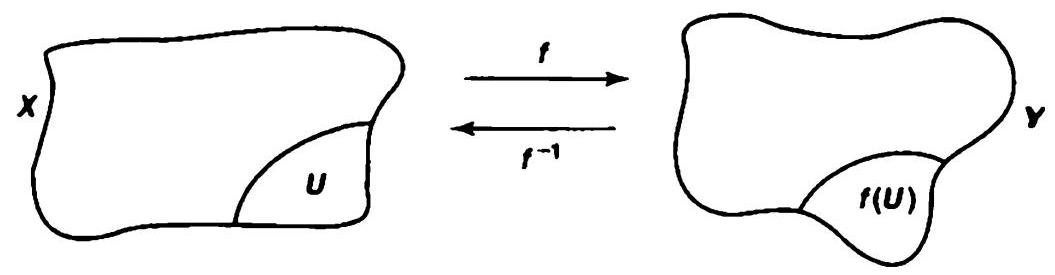
\includegraphics[width=0.9\textwidth]{images/18.1.jpg}
\end{center}
\hspace*{3em} 

Figure 18.1

This remark shows that a homeomorphism \(f : X \rightarrow  Y\) gives us a bijective correspondence not only between \(X\) and \(Y\) but between the collections of open sets of \(X\) and of \(Y\) . As a result, any property of \(X\) that is entirely expressed in terms of the topology of \(X\) (that is, in terms of the open sets of \(X\) ) yields, via the correspondence \(f\) , the corresponding property for the space \(Y\) . Such a property of \(X\) is called a \index{topological property} of \(X\) .

You may have studied in modern algebra the notion of an \index{isomorphism} between algebraic objects such as groups or rings. An isomorphism is a bijective correspondence that preserves the algebraic structure involved. The analogous concept in topology is that of homeomorphism; it is a bijective correspondence that preserves the topological structure involved.

Now suppose that \(f : X \rightarrow  Y\) is an injective continuous map, where \(X\) and \(Y\) are topological spaces. Let \(Z\) be the image set \(f( X)\) , considered as a subspace of \(Y\) ; then the function \({f}^{\prime } : X \rightarrow  Z\) obtained by restricting the range of \(f\) is bijective. If \({f}^{\prime }\) happens to be a homeomorphism of \(X\) with \(Z\) , we say that the map \(f : X \rightarrow  Y\) is a topological \index{imbedding}, or simply an imbedding, of \(X\) in \(Y\) .

\begin{centeredblock}
\begin{example}
	The function \(f : \mathbb{R} \rightarrow  \mathbb{R}\) given by \(f( x)  = {3x} + 1\) is a homeomorphism See Figure 18 2. If we define \(g \cdot  \mathbb{R} \rightarrow  \mathbb{R}\) by the equation

\[
g( y)  = \frac{1}{3}( {y - 1})
\]

then one can check easily that \(f( {g( y) })  = y\) and \(g( {f( x) })  = x\) for all real numbers \(x\) and \(y\) It follows that \(f\) is bijective and that \(g = {f}^{-1}\) , the continuity of \(f\) and \(g\) is a familiar result from calculus.
\end{example}
\end{centeredblock}

\begin{centeredblock}
\begin{example}
	The function \(F : ( {-1,1})  \rightarrow  \mathbb{R}\) defined by

\[
F( x)  = \frac{x}{1 - {x}^{2}}
\]

is a homeomorphism See Figure 18.3 We have already noted in Example 9 of \(§3\) that \(F\) is a bijective order-preserving correspondence, its inverse is the function \(G\) defined by

\[
G( y)  = \frac{2y}{1 + {( 1 + 4{y}^{2}) }^{1/2}}.
\]

The fact that \(F\) is a homeomorphism can be proved in two ways One way is to note that because \(F\) is order preserving and bijective, \(F\) carnes a basis element for the order topology in(-1,1)onto a basis element for the order topology in \(\mathbb{R}\) and vice versa As a result, \(F\) is automatically a homeomorphism of(-1,1)with \(\mathbb{R}\) (both in the order topology) Since the order topology on(-1,1)and the usual (subspace) topology agree, \(F\) is a homeomorphism of(-1,1)with \(\mathbb{R}\)

\begin{center}
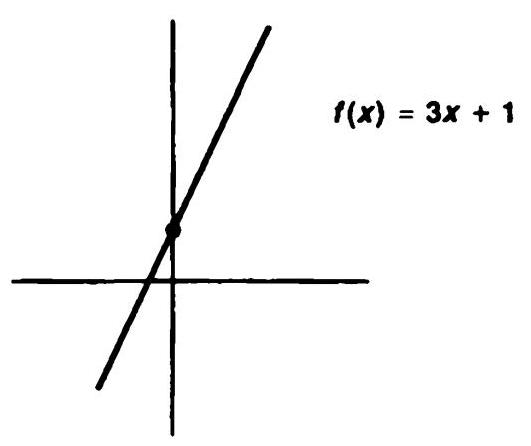
\includegraphics[width=0.4\textwidth]{images/18.2.jpg}
\end{center}
\hspace*{3em}

Figure 18.2

\begin{center}
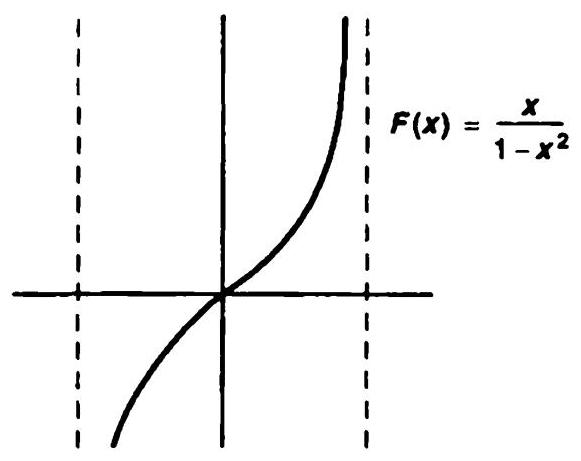
\includegraphics[width=0.5\textwidth]{images/18.3.jpg}
\end{center}
\hspace*{3em}

Figure 18.3

A second way to show \(F\) a homeomorphism is to use the continuity of the algebraic functions and the square-root function to show that both \(F\) and \(G\) are continuous These are familiar facts from calculus
\end{example}
\end{centeredblock}

\begin{centeredblock}
\begin{example}
	A bijective function \(f : X \rightarrow  Y\) can be continuous without being a homeomorphism One such function is the identity map \(g\;{\mathbb{R}}_{\ell } \rightarrow  \mathbb{R}\) considered in Example 3 Another is the following Let \(\index{S@\({S}^{1}\)} \index{S@${S}^{1}$}{S}^{1}\) denote the unit circle.

\[
{S}^{1} = \{  {x \times  y \mid  {x}^{2} + {y}^{2} = 1}\}  ,
\]

considered as a subspace of the plane \({\mathbb{R}}^{2}\) , and let

\[
F \cdot  \lbrack 0,1) \rightarrow  {S}^{1}
\]

be the map defined by \(f( t)  = ( {\cos {2\pi t},\sin {2\pi t}})\) . The fact that \(f\) is bijective and continuous follows from famuliar properties of the trigonometric functions. But the function \({f}^{-1}\) is not continuous The image under \(f\) of the open set \(U = [  {0,\frac{1}{4}})\) of the domain, for instance, is not open in \({S}^{1}\) , for the point \(p = f( 0)\) lies in no open set \(V\) of \({\mathbb{R}}^{2}\) such that \(V \cap  {S}^{1} \subset  f( U)\) . See Figure 18.4.

\begin{center}
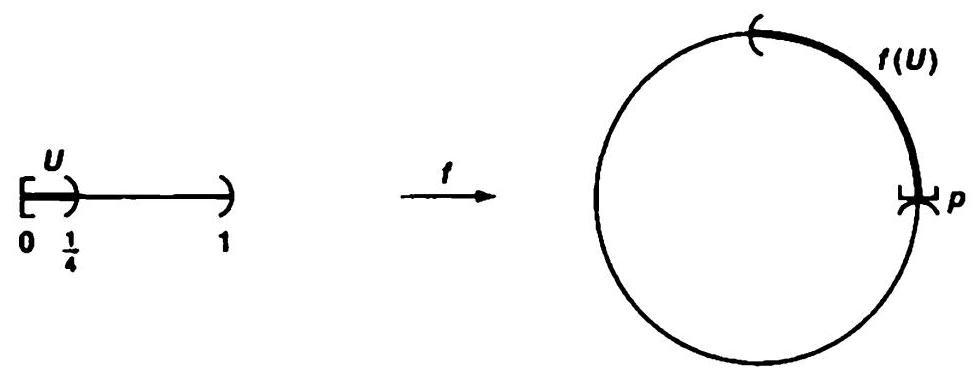
\includegraphics[width=0.9\textwidth]{images/18.4.jpg}
\end{center}
\hspace*{3em} 

Figure 18.4
\end{example}
\end{centeredblock}

\begin{centeredblock}
\begin{example}
	Consider the function

\[
g : \lbrack 0,1) \rightarrow  {\mathbb{R}}^{2}
\]

obtained from the function \(f\) of the preceding example by expanding the range. The map \(g\) is an example of a continuous injective map that is not an \index{Imbedding}imbedding
\end{example}
\end{centeredblock}

\section*{Constructing Continuous Functions}

How does one go about constructing continuous functions from one topological space to another? There are a number of methods used in analysis, of which some generalize to arbitrary topological spaces and others do not. We study first some constructions that do hold for general topological spaces, deferring consideration of the others until later.

\begin{theorem}[Rules for constructing continuous functions]
	Let \(X,Y\) , and \(Z\) be topological spaces.

(a) (Constant function) If \(f : X \rightarrow  Y\) maps all of \(X\) into the single point \({y}_{O}\) of \(Y\) , then \(f\) is continuous.

(b) (Inclusion) If \(A\) is a subspace of \(X\) , the inclusion function \(j : A \rightarrow  X\) is continuous.

(c) (\index{Quotient map!composites}Composites) If \(f : X \rightarrow  Y\) and \(g : Y \rightarrow  Z\) are continuous, then the map \(g \circ  f : X \rightarrow  Z\) is continuous.

(d) (Restricting the domain) If \(f : X \rightarrow  Y\) is continuous, and if \(A\) is a subspace of \(X\) , then the restricted function \(f \mid  A \cdot  A \rightarrow  Y\) is continuous.

(e) (Restricting or expanding the range) Let \(f \cdot  X \rightarrow  Y\) be continuous. If \(Z\) is a subspace of \(Y\) containing the image set \(f( X)\) , then the function \(g : X \rightarrow  Z\) obtained by restricting the range of \(f\) is continuous. If \(Z\) is a space having \(Y\) as a subspace, then the function \(h : X \rightarrow  Z\) obtained by expanding the range of \(f\) is continuous.

(f) (\index{Continuity: of algebraic operations in \(\mathbb{R}\)!local formulation}Local formulation of continuity) The map \(f : X \rightarrow  Y\) is continuous if \(X\) can be written as the union of open sets \({U}_{\alpha }\) such that \(f \mid  {U}_{\alpha }\) is continuous for each \(\alpha\) .

\end{theorem}
\begin{proof}
(a) Let \(f( x)  = {y}_{0}\) for every \(x\) in \(X\) . Let \(V\) be open in \(Y\) . The set \({f}^{-1}( V)\) equals \(X\) or \(\varnothing\) , depending on whether \(V\) contains \({y}_{0}\) or not. In either case, it is open.

(b) If \(U\) is open in \(X\) , then \({j}^{-1}( U)  = U \cap  A\) , which is open in \(A\) by definition of the subspace topology.

(c) If \(U\) is open in \(Z\) , then \({g}^{-1}( U)\) is open in \(Y\) and \({f}^{-1}( {{g}^{-1}( U) })\) is open in \(X\) . But

\[
{f}^{-1}( {{g}^{-1}( U) })  = {( g \circ  f) }^{-1}( U) ,
\]

by elementary set theory.

(d) The function \(f \mid  A\) equals the composite of the inclusion map \(j : A \rightarrow  X\) and the map \(f : X \rightarrow  Y\) , both of which are continuous.

(e) Let \(f : X \rightarrow  Y\) be continuous. If \(f( X)  \subset  Z \subset  Y\) , we show that the function \(g : X \rightarrow  Z\) obtained from \(f\) is continuous. Let \(B\) be open in \(Z\) . Then \(B = Z \cap  U\) for some open set \(U\) of \(Y\) . Because \(Z\) contains the entire image set \(f( X)\) ,

\[
{f}^{-1}( U)  = {g}^{-1}( B) ,
\]

by elementary set theory. Since \({f}^{-1}( U)\) is open, so is \({g}^{-1}( B)\) .

To show \(h : X \rightarrow  Z\) is continuous if \(Z\) has \(Y\) as a subspace, note that \(h\) is the composite of the map \(f : X \rightarrow  Y\) and the inclusion map \(j : Y \rightarrow  Z\) .

(f) By hypothesis, we can write \(X\) as a union of open sets \({U}_{\alpha }\) , such that \(f \mid  {U}_{\alpha }\) is continuous for each \(\alpha\) . Let \(V\) be an open set in \(Y\) . Then

\[
{f}^{-1}( V)  \cap  {U}_{\alpha } = {( f \mid  {U}_{\alpha }) }^{-1}( V) ,
\]

because both expressions represent the set of those points \(x\) lying in \({U}_{\alpha }\) for which \(f( x)  \in  V\) . Since \(f \mid  {U}_{\alpha }\) is continuous, this set is open in \({U}_{\alpha }\) , and hence open in \(X\) But

\[
{f}^{-1}( V)  = \mathop{\bigcup }\limits_{\alpha }( {{f}^{-1}( V)  \cap  {U}_{\alpha }})
\]

so that \({f}^{-1}( V)\) is also open in \(X\) .
\end{proof}

\begin{theorem}[The \index{pasting lemma}]
	Let \(X = A \cup  B\) , where \(A\) and \(B\) are closed in \(X\) . Let \(f : A \rightarrow  Y\) and \(g : B \rightarrow  Y\) be continuous. If \(f( x)  = g( x)\) for every \(x \in  A \cap  B\) , then \(f\) and \(g\) combine to give a continuous function \(h : X \rightarrow  Y\) , defined by setting \(h( x)  = f( x)\) if \(x \in  A\) , and \(h( x)  = g( x)\) if \(x \in  B\) .
\end{theorem}
\begin{proof}
	Let \(C\) be a closed subset of \(Y\) . Now

\[
{h}^{-1}( C)  = {f}^{-1}( C)  \cup  {g}^{-1}( C) ,
\]

by elementary set theory. Since \(f\) is continuous, \({f}^{-1}( C)\) is closed in \(A\) and, therefore, closed in \(X\) . Similarly, \({g}^{-1}( C)\) is closed in \(B\) and therefore closed in \(X\) . Their union \({h}^{-1}( C)\) is thus closed in \(X\) .

This theorem also holds if \(A\) and \(B\) are open sets in \(X\) ; this is just a special case of the ``local formulation of continuity'' rule given in preceding theorem.

\begin{centeredblock}
\begin{example}
	Let us define a function \(h : \mathbb{R} \rightarrow  \mathbb{R}\) by setting

\[
h( x)  = \{  \begin{array}{ll} x & \text{ for }x \leq  0 \\  x/2 & \text{ for }x \geq  0 \end{array}.
\]

Each of the ``pieces'' of this definition is a continuous function, and they agree on the overlapping part of their domains, which is the one-point set \(\{ 0\}\) . Since their domains are closed in \(\mathbb{R}\) , the function \(h\) is continuous. One needs the ``pieces'' of the function to agree on the overlapping part of their domains in order to have a function at all. The equations

\[
k( x)  = \{  \begin{array}{ll} x - 2 & \text{ for }x \leq  0, \\  x + 2 & \text{ for }x \geq  0, \end{array}.
\]

for instance, do not define a function On the other hand, one needs some limitations on the sets \(A\) and \(B\) to guarantee continuity. The equations

\[
l( x)  = \{  \begin{array}{ll} x - 2 & \text{ for }x < 0, \\  x + 2 & \text{ for }x \geq  0, \end{array}.
\]

for instance, do define a function \(l\) mapping \(\mathbb{R}\) into \(\mathbb{R}\) , and both of the pieces are continuous. But \(l\) is not continuous; the inverse image of the open set(1,3), for instance, is the nonopen set \(\lbrack 0,1)\) See Figure 18.5

\begin{center}
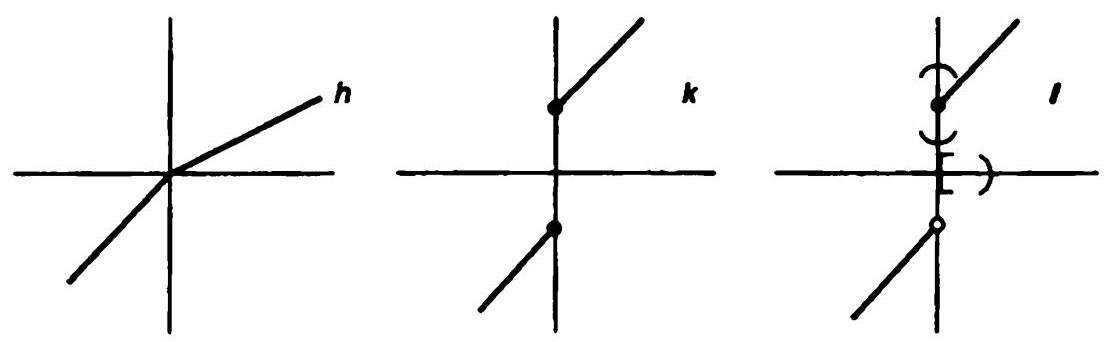
\includegraphics[width=1.0\textwidth]{images/18.5.jpg}
\end{center}
\hspace*{3em}

Figure 18.5
\end{example}
\end{centeredblock}

\end{proof}
\begin{theorem}[Maps into products]
	Let \(f : A \rightarrow  X \times  Y\) be given by the equation

\[
f( a)  = ( {{f}_{1}( a) ,{f}_{2}( a) }) .
\]

Then \(f\) is continuous if and only if the functions

\[
{f}_{1} : A \rightarrow  X\;\text{ and }\;{f}_{2} : A \rightarrow  Y
\]

are continuous.

The maps \({f}_{1}\) and \({f}_{2}\) are called the \index{coordinate function} of \(f\) .

\end{theorem}
\begin{proof}
Let \({\pi }_{1}.X \times  Y \rightarrow  X\) and \({\pi }_{2} : X \times  Y \rightarrow  Y\) be projections onto the first and second factors, respectively. These maps are continuous. For \({\pi }_{1}^{-1}( U)  = U \times  Y\) and \({\pi }_{2}^{-1}( V)  = X \times  V\) , and these sets are open if \(U\) and \(V\) are open. Note that for each \(a \in  A\) ,

\[
{f}_{1}( a)  = {\pi }_{1}( {f( a) }) \;\text{ and }\;{f}_{2}( a)  = {\pi }_{2}( {f( a) }) .
\]

If the function \(f\) is continuous, then \({f}_{1}\) and \({f}_{2}\) are composites \index{Composite: of functions!of continuous functions}of continuous functions and therefore continuous. Conversely, suppose that \({f}_{1}\) and \({f}_{2}\) are continuous. We show that for each basis element \(U \times  V\) for the topology of \(X \times  Y\) , its inverse image \({f}^{-1}( {U \times  V})\) is open. A point \(a\) is in \({f}^{-1}( {U \times  V})\) if and only if \(f( a)  \in  U \times  V\) , that is, if and only if \({f}_{1}( a)  \in  U\) and \({f}_{2}( a)  \in  V\) . Therefore,

\[
{f}^{-1}( {U \times  V})  = {f}_{1}^{-1}( U)  \cap  {f}_{2}^{-1}( V) .
\]

Since both of the sets \({f}_{1}^{-1}( U)\) and \({f}_{2}^{-1}( V)\) are open, so is their intersection.

There is no useful criterion for the continuity of a map \(f : A \times  B \rightarrow  X\) whose domain is a \index{Product space}product space. One might conjecture that \(f\) is continuous if it is continuous ``in each variable separately,'' but this conjecture is not true. (See Exercise 12.)
\end{proof}

\begin{centeredblock}
\begin{example}
	In calculus, a parametrized curve in the plane is defined to be a continuous map \(f[  {a,b}]   \rightarrow  {\mathbb{R}}^{2}\) It is often expressed in the form \(f( t)  = ( {x( t) ,y( t) })\) ; and one frequently uses the fact that \(f\) is a continuous function of \(t\) if both \(x\) and \(y\) are Similarly, a vector field in the plane

\[
\mathbf{v}( {x,y})  = P( {x,y}) \mathbf{i} + Q( {x,y}) \mathbf{j}
\]

\[
= ( {P( {x,y}) ,Q( {x,y}) })
\]

is said to be continuous if both \(P\) and \(Q\) are continuous functions, or equivalently, if \(\mathbf{v}\) is continuous as a map of \({\mathbb{R}}^{2}\) into \({\mathbb{R}}^{2}\) . Both of these statements are simply special cases of the preceding theorem.
\end{example}
\end{centeredblock}

One way of forming continuous functions that is used a great deal in analysis is to take sums, differences, products, or \index{Quotient space (see also Quotient topology)} quotients of continuous real-valued functions. It is a standard theorem that if \(f.g.X \rightarrow  \mathbb{R}\) are continuous, then \(f + g,f - g\) , and \(f \cdot  g\) are continuous, and \(f/g\) is continuous if \(g( x)  \neq  0\) for all \(x\) . We shall consider this theorem in \(§{21}\) .

Yet another method for constructing continuous functions that is familiar from analysis is to take the limit of an infinite sequence of functions. There is a theorem to the effect that if a sequence of continuous real-valued functions of a real variable converges \index{Uniform metric (see also Uniform topology)} uniformly to a limit function, then the limit function is necessarily continuous. This theorem is called the \index{Uniform Limit Theorem}. It is used, for instance, to demonstrate the continuity of the trigonometric functions, when one defines these functions rigorously using the infinite series definitions of the sine and cosine. This theorem generalizes to a theorem about maps of an arbitrary topological space \(X\) into a metric space \(Y\) . We shall prove it in \(§{21}\) .

\section*{Exercises}
\begin{enumerate}[itemsep=0.4em, parsep=0pt, topsep=0pt, partopsep=0pt, leftmargin=*, label=\arabic*., ref=\arabic*]
\item Prove that for functions \(f : \mathbb{R} \rightarrow  \mathbb{R}\) , the \(\epsilon  - \delta\) definition of continuity implies the open set definition.
\item Suppose that \(f : X \rightarrow  Y\) is continuous. If \(x\) is a limit point of the subset \(A\) of \(X\) , is it necessarily true that \(f( x)\) is a limit point of \(f( A)\) ?
\item Let \(X\) and \({X}^{\prime }\) denote a single set in the two topologies \(\mathcal{T}\) and \({\mathcal{T}}^{\prime }\) , respectively. Let \(i : {X}^{\prime } \rightarrow  X\) be the identity function.
  \begin{enumerate}[itemsep=0.2em, parsep=0pt, topsep=0pt, partopsep=0pt, leftmargin=*, label=(\alph*), align=left]
  \item Show that \(i\) is continuous \(\Leftrightarrow  {\mathcal{T}}^{\prime }\) is finer than \(\mathcal{T}\) .
  \item Show that \(i\) is a homeomorphism \(\Leftrightarrow  {\mathcal{T}}^{\prime } = \mathcal{T}\) .
  \end{enumerate}
\item Given \({x}_{0} \in  X\) and \({y}_{0} \in  Y\) , show that the maps \(f : X \rightarrow  X \times  Y\) and \(g : Y \rightarrow\)  \(X \times  Y\) defined by \[ f( x)  = x \times  {y}_{0}\;\text{ and }\;g( y)  = {x}_{0} \times  y \] are imbeddings.
\item Show that the subspace(a, b)of \(\mathbb{R}\) is homeomorphic with(0,1)and the subspace \([  {a,b}]\) of \(\mathbb{R}\) is homeomorphic with \([  {0,1}]\)
\item Find a function \(f : \mathbb{R} \rightarrow  \mathbb{R}\) that is continuous at precisely one point.
\item
  \begin{enumerate}[itemsep=0.2em, parsep=0pt, topsep=0pt, partopsep=0pt, leftmargin=*, label=(\alph*), align=left]
  \item Suppose that \(f : \mathbb{R} \rightarrow  \mathbb{R}\) is ``continuous from the right,'' that is, \[ \mathop{\lim }\limits_{{x \rightarrow  {a}^{ + }}}f( x)  = f( a) \] for each \(a \in  \mathbb{R}\) . Show that \(f\) is continuous when considered as a function from \({\mathbb{R}}_{\ell }\) to \(\mathbb{R}\) .

  \item Can you conjecture what functions \(f \cdot  \mathbb{R} \rightarrow  \mathbb{R}\) are continuous when considered as maps from \(\mathbb{R}\) to \({\mathbb{R}}_{\ell }\) ? As maps from \({\mathbb{R}}_{\ell }\) to \({\mathbb{R}}_{\ell }\) ? We shall return to this question in Chapter 3.
  \end{enumerate}
\item Let \(Y\) be an ordered set in the order topology. Let \(f,g : X \rightarrow  Y\) be continuous. (a) Show that the set \(\{ x \mid  f( x)  \leq  g( x) \}\) is closed in \(X\)
  \begin{enumerate}[itemsep=0.2em, parsep=0pt, topsep=0pt, partopsep=0pt, leftmargin=*, label=(\alph*), align=left]
  \item Let \(h : X \rightarrow  Y\) be the function \[ h( x)  = \min \{ f( x) ,g( x) \} . \] Show that \(h\) is continuous [Hint: Use the \index{Pasting lemma}pasting lemma.]
  \end{enumerate}
\item Let \(\{  {A}_{\alpha }\}\) be a collection of subsets of \(X\) ; let \(X = \mathop{\bigcup }\limits_{\alpha }{A}_{\alpha }\) . Let \(f : X \rightarrow  Y\) ; suppose that \(f \mid  {A}_{\alpha }\) , is continuous for each \(\alpha\) .
  \begin{enumerate}[itemsep=0.2em, parsep=0pt, topsep=0pt, partopsep=0pt, leftmargin=*, label=(\alph*), align=left]
  \item Show that if the collection \(\{  {A}_{\alpha }\}\) is finite and each set \({A}_{\alpha }\) is closed, then \(f\) is continuous.
  \item Find an example where the collection \(\{  {A}_{\alpha }\}\) is countable and each \({A}_{\alpha }\) is closed, but \(f\) is not continuous.
  \item An indexed family of sets \(\{  {A}_{\alpha }\}\) is said to be \index{Locally finite family} locally finite if each point \(x\) of \(X\) has a neighborhood that intersects \({A}_{\alpha }\) for only finitely many values of \(\alpha\) . Show that if the family \(\{  {A}_{\alpha }\}\) is locally finite and each \({A}_{\alpha }\) is closed, then \(f\) is continuous.
  \end{enumerate}
\item Let \(f \cdot  A \rightarrow  B\) and \(g : C \rightarrow  D\) be continuous functions. Let us define a map \(f \times  g : A \times  C \rightarrow  B \times  D\) by the equation \[ ( {f \times  g}) ( {a \times  c})  = f( a)  \times  g( c) . \] Show that \(f \times  g\) is continuous.
\item Let \(F : X \times  Y \rightarrow  Z\) . We say that \(F\) is continuous in each variable separately if for each \({y}_{0}\) in \(Y\) , the map \(h : X \rightarrow  Z\) defined by \(h( x)  = F( {x \times  {y}_{0}})\) is continuous, and for each \({x}_{0}\) in \(X\) , the map \(k \cdot  Y \rightarrow  Z\) defined by \(k( y)  = F( {{x}_{0} \times  y})\) is continuous. Show that if \(F\) is continuous, then \(F\) is continuous in each variable separately.
\item Let \(F : \mathbb{R} \times  \mathbb{R} \rightarrow  \mathbb{R}\) be defined by the equation \[ F( {x \times  y})  = \{  \begin{array}{ll} {xy}/( {{x}^{2} + {y}^{2}}) & \text{ if }x \times  y \neq  0 \times  0. \\  0 & \text{ if }x \times  y = 0 \times  0 \end{array}. \]
  \begin{enumerate}[itemsep=0.2em, parsep=0pt, topsep=0pt, partopsep=0pt, leftmargin=*, label=(\alph*), align=left]
  \item Show that \(F\) is continuous in each variable separately.
  \item Compute the function \(g : \mathbb{R} \rightarrow  \mathbb{R}\) defined by \(g( x)  = F( {x \times  x})\) .
  \item Show that \(F\) is not continuous
  \end{enumerate}
\item Let \(A \subset  X\) ; let \(f : A \rightarrow  Y\) be continuous; let \(Y\) be Hausdorff. Show that if \(f\) may be extended to a continuous function \(g.\bar{A} \rightarrow  Y\) , then \(g\) is uniquely determined by \(f\)
\end{enumerate}
\section*{§ 19 The Product Topology}

We now return, for the remainder of the chapter, to the consideration of various methods for imposing topologies on sets

Previously, we defined a topology on the product \(X \times  Y\) of two topological spaces. In the present section, we generalize this definition to more general cartesian products.

So let us consider the cartesian products

\[
{X}_{1} \times  \cdots  \times  {X}_{n}\;\text{ and }\;{X}_{1} \times  {X}_{2} \times  \cdots ,
\]

where each \({X}_{i}\) is a topological space There are two possible ways to proceed. One way is to take as basis all sets of the form \({U}_{1} \times  \cdots  \times  {U}_{n}\) in the first case, and of the form \({U}_{1} \times  {U}_{2} \times  \cdots\) in the second case, where \({U}_{i}\) is an open set of \({X}_{i}\) for each \(i\) . This procedure does indeed define a topology on the cartesian product; we shall call it the \index{box topology}.

Another way to proceed is to generalize the subbasis formulation of the definition, given in \(§{15}\) . In this case, we take as a subbasis all sets of the form \({\pi }_{i}^{-1}( {U}_{i})\) , where \(i\) is any index and \({U}_{i}\) is an open set of \({X}_{i}\) . We shall call this topology the product topology.

How do these topologies differ? Consider the typical basis element \(B\) for the second topology. It is a finite intersection of subbasis elements \({\pi }_{i}^{-1}( {U}_{i})\) , say for \(i =\)  \({i}_{1},\ldots ,{i}_{k}\) . Then a point \(\mathbf{x}\) belongs to \(B\) if and only if \({\pi }_{i}( \mathbf{x})\) belongs to \({U}_{i}\) for \(i =\)  \({i}_{1},\ldots ,{i}_{k}\) ; there is no restriction on \({\pi }_{i}( x)\) for other values of \(i\) .

It follows that these two topologies agree for the finite cartesian product and differ for the infinite product. What is not clear is why we seem to prefer the second topology. This is the question we shall explore in this section

Before proceeding, however, we shall introduce a more general notion of cartesian product. So far, we have defined the cartesian product of an indexed family of sets only in the cases where the index set was the set \(\{ 1,\ldots ,n\}\) or the set \({\mathbb{Z}}_{ + }\) Now we consider the case where the index set is completely arbitrary.

\begin{definition}
	Let \(J\) be an index set. Given a set \(X\) , we define a \(J\) -tuple of elements of \(X\) to be a function \(\mathbf{x} : J \rightarrow  X\) . If \(\alpha\) is an element of \(J\) , we often denote the value of \(x\) at \(\alpha\) by \({x}_{\alpha }\) rather than \(x( \alpha )\) ; we call it the \(\alpha\) th coordinate of \(x\) . And we often denote the function \(x\) itself by the symbol

\[
{( {x}_{\alpha }) }_{\alpha  \in  J},
\]

which is as close as we can come to a ``tuple notation'' for an arbitrary index set \(J\) . We denote the set of all \(J\) -tuples of elements of \(X\) by \(\index{X@\({X}^{J}\)} \index{X@${X}^{J}$}{X}^{J}\) .
\end{definition}

\begin{definition}
	Let \({\{  {A}_{\alpha }\}  }_{\alpha  \in  J}\) be an indexed family of sets; let \(X = \mathop{\bigcup }\limits_{{\alpha  \in  J}}{A}_{\alpha }\) . The cartesian product of this indexed family, denoted by

\[
\mathop{\prod }\limits_{{\alpha  \in  J}}{A}_{\alpha }
\]

is defined to be the set of all \(J\) -tuples \({( {x}_{\alpha }) }_{\alpha  \in  J}\) of elements of \(X\) such that \({x}_{\alpha } \in  {A}_{\alpha }\) for each \(\alpha  \in  J\) That is, it is the set of all functions

\[
\mathbf{x} : J \rightarrow  \mathop{\bigcup }\limits_{{\alpha  \in  J}}{A}_{\alpha }
\]

such that \(\mathbf{x}( \alpha )  \in  {A}_{\alpha }\) for each \(\alpha  \in  J\) .

Occasionally we denote the product simply by \(\prod {A}_{\alpha }\) , and its general element by \(( {x}_{\alpha })\) , if the index set is understood
\end{definition}

If all the sets \({A}_{\alpha }\) are equal to one set \(X\) , then the cartesian product \(\mathop{\prod }\limits_{{\alpha  \in  J}}{A}_{\alpha }\) is just the set \({X}^{J}\) of all \(J\) -tuples of elements of \(X\) . We sometimes use ``tuple notation'' for the elements of \({X}^{J}\) , and sometimes we use functional notation, depending on which is more convenient.

\begin{definition}
	Let \({\{  {X}_{\alpha }\}  }_{\alpha  \in  J}\) be an indexed family of topological spaces. Let us take as a basis for a topology on the product space

\[
\mathop{\prod }\limits_{{\alpha  \in  J}}{X}_{\alpha }
\]

the collection of all sets of the form

\[
\mathop{\prod }\limits_{{\alpha  \in  J}}{U}_{\alpha }
\]

where \({U}_{\alpha }\) is open in \({X}_{\alpha }\) , for each \(\alpha  \in  J\) . The topology generated by this basis is called the \index{Box topology}box topology
\end{definition}

This collection satisfies the first condition for a basis because \(\prod {X}_{\alpha }\) is itself a basis element; and it satisfies the second condition because the intersection of any two basis elements is another basis element.

\[
( {\mathop{\prod }\limits_{{\alpha  \in  J}}{U}_{\alpha }})  \cap  ( {\mathop{\prod }\limits_{{\alpha  \in  J}}{V}_{\alpha }})  = \mathop{\prod }\limits_{{\alpha  \in  J}}( {{U}_{\alpha } \cap  {V}_{\alpha }}) .
\]

Now we generalize the subbasis formulation of the definition. Let

\[
{\pi }_{\beta } : \mathop{\prod }\limits_{{\alpha  \in  J}}{X}_{\alpha } \rightarrow  {X}_{\beta }
\]

be the function assigning to each element of the product space its \(\beta\) th coordinate,

\[
{\pi }_{\beta }( {( {x}_{\alpha }) }_{\alpha  \in  J})  = {x}_{\beta };
\]

it is called the \index{projection map}ing associated with the index \(\beta\) .

\begin{definition}
	Let \({S}_{\beta }\) denote the collection

\[
{S}_{\beta } = \{  {{\pi }_{\beta }^{-1}( {U}_{\beta })  \mid  {U}_{\beta }\text{ open in }{X}_{\beta }}\}  ,
\]

and let \(S\) denote the union of these collections,

\[
S = \mathop{\bigcup }\limits_{{\beta  \in  J}}{S}_{\beta }
\]

The topology generated by the subbasis \(S\) is called the product topology. In this topology \(\mathop{\prod }\limits_{{\alpha  \in  J}}{X}_{\alpha }\) is called a product space.
\end{definition}

To compare these topologies, we consider the basis \(\mathcal{B}\) that \(\mathcal{S}\) generates. The collection \(\mathcal{B}\) consists of all finite intersections of elements of \(\mathcal{S}\) . If we intersect elements belongingg to the same one of the sets \({S}_{\beta }\) , we do not get anything new, because

\[
{\pi }_{\beta }^{-1}( {U}_{\beta })  \cap  {\pi }_{\beta }^{-1}( {V}_{\beta })  = {\pi }_{\beta }^{-1}( {{U}_{\beta } \cap  {V}_{\beta }})
\]

the intersection of two elements of \({S}_{\beta }\) , or of finitely many such elements, is again an element of \({S}_{\beta }\) . We get something new only when we intersect elements from different sets \({S}_{\beta }\) . The typical element of the basis \(\mathcal{B}\) can thus be described as follows \(\ldots ,{\beta }_{n}\) be a finite set of distinct indices from the index set \(J\) , and let \({U}_{{\beta }_{i}}\) be an open set in \({X}_{{\beta }_{i}}\) for \(i = 1,\ldots ,n\) . Then

\[
B = {\pi }_{{\beta }_{1}}^{-1}( {U}_{{\beta }_{1}})  \cap  {\pi }_{{\beta }_{2}}^{-1}( {U}_{{\beta }_{2}})  \cap   \cdot   \cap  {\pi }_{{\beta }_{n}}^{-1}( {U}_{{\beta }_{n}})
\]

is the typical element of \(\mathcal{B}\) .

Now a point \(\mathbf{x} = ( {x}_{\alpha })\) is in \(B\) if and only if its \({\beta }_{1}\) th coordinate is in \({U}_{{\beta }_{1}}\) , its \({\beta }_{2}\) th coordinate is in \({U}_{{\beta }_{2}}\) , and so on. There is no restriction whatever on the \(\alpha\) th coordinate of \(\mathbf{x}\) if \(\alpha\) is not one of the indices \({\beta }_{1},\ldots ,{\beta }_{n}\) . As a result, we can write \(B\) as the product

\[
B = \mathop{\prod }\limits_{{\alpha  \in  J}}{U}_{\alpha }
\]

where \({U}_{\alpha }\) denotes the entire space \({X}_{\alpha }\) if \(\alpha  \neq  {\beta }_{1},\ldots ,{\beta }_{n}\) .

All this is summarized in the following theorem:

\begin{theorem}[Comparison of the box and product topologies]
	The box topology on \(\prod {X}_{\alpha }\) has as basis all sets of the form \(\prod {U}_{\alpha }\) , where \({U}_{\alpha }\) is open in \({X}_{\alpha }\) for each \(\alpha\) . The product topology on \(\prod {X}_{\alpha }\) has as basis all sets of the form \(\prod {U}_{\alpha }\) , where \({U}_{\alpha }\) is open in \({X}_{\alpha }\) for each \(\alpha\) and \({U}_{\alpha }\) equals \({X}_{\alpha }\) except for finitely many values of \(\alpha\) .

Two things are immediately clear First, for finite products \(\mathop{\prod }\limits_{{\alpha  = 1}}^{n}{X}_{\alpha }\) the two topologies are precisely the same. Second, the box topology is in general finer than the product topology.

What is not so clear is why we prefer the product topology to the box topology. The answer will appear as we continue our study of topology. We shall find that a number of important theorems about finite products will also hold for arbitrary products if we use the product topology, but not if we use the box topology. As a result, the product topology is extremely important in mathematics. The box topology is not so important; we shall use it primarily for constructing counterexamples. Therefore, we make the following convention:

Whenever we consider the product \(\prod {X}_{\alpha }\) , we shall assume it is given the product topology unless we specifically state otherwise.

Some of the theorems we proved for the product \(X \times  Y\) hold for the product \(\prod {X}_{\alpha }\) no matter which topology we use. We list them here; most of the proofs are left to the exercises.

\end{theorem}
\begin{theorem}
	Suppose the topology on each space \({X}_{\alpha }\) is given by a basis \({\mathcal{B}}_{\alpha }\) . The collection of all sets of the form

\[
\mathop{\prod }\limits_{{\alpha  \in  J}}{B}_{\alpha }
\]

where \({B}_{\alpha } \in  {\mathcal{B}}_{\alpha }\) for each \(\alpha\) , will serve as a basis for the box topology on \(\mathop{\prod }\limits_{{\alpha  \in  J}}{X}_{\alpha }\) .

The collection of all sets of the same form, where \({B}_{\alpha } \in  {\mathcal{B}}_{\alpha }\) for finitely many indices \(\alpha\) and \({B}_{\alpha } = {X}_{\alpha }\) for all the remaining indices, will serve as a basis for the \(\begin{matrix} \text{ product topology }\mathop{\prod }\limits_{{\alpha  \in  J}}{X}_{\alpha }. \end{matrix}\)

\begin{centeredblock}
\begin{example}
	Consider euclidean \(n\) -space \({\mathbb{R}}^{n}\) . A basis for \(\mathbb{R}\) consists of all open intervals in \(\mathbb{R}\) ; hence a basis for the topology of \({\mathbb{R}}^{n}\) consists of all products of the form

\[
( {{a}_{1},{b}_{1}})  \times  ( {{a}_{2},{b}_{2}})  \times   \cdot  \; \times  ( {{a}_{n},{b}_{n}}) .
\]

Since \({\mathbb{R}}^{n}\) is a finite product, the box and product topologies agree Whenever we consider \({\mathbb{R}}^{n}\) , we will assume that it is given this topology, unless we specifically state otherwise
\end{example}
\end{centeredblock}

\end{theorem}
\begin{theorem}
	Let \({A}_{\alpha }\) be a subspace of \({X}_{\alpha }\) , for each \(\alpha  \in  J\) . Then \(\prod {A}_{\alpha }\) is a subspace of \(\prod {X}_{\alpha }\) if both products are given the box topology, or if both products are given the product topology.

\end{theorem}
\begin{theorem}
	If each space \({X}_{\alpha }\) is a Hausdorff space, then \(\prod {X}_{\alpha }\) is a Hausdorff space in both the box and product topologies.

\end{theorem}
\begin{theorem}
	Let \(\{  {X}_{\alpha }\}\) be an indexed family of spaces; let \({A}_{\alpha } \subset  {X}_{\alpha }\) for each \(\alpha\) . If \(\prod {X}_{\alpha }\) is given either the product or the box topology, then

\[
\prod {\widetilde{A}}_{\alpha } = \bar{\prod }\overline{{A}_{\alpha }}.
\]

\end{theorem}
\begin{proof}
Let \(\mathbf{x} = ( {x}_{\alpha })\) be a point of \(\prod {\bar{A}}_{\alpha }\) ; we show that \(\mathbf{x} \in  \overline{\prod {A}_{\alpha }}\) . Let \(U = \prod {U}_{\alpha }\) be a basis element for either the box or product topology that contains \(\mathbf{x}\) . Since \({x}_{\alpha } \in  {\widetilde{A}}_{\alpha }\) , we can choose a point \({y}_{\alpha } \in  {U}_{\alpha } \cap  {A}_{\alpha }\) for each \(\alpha\) . Then \(\mathbf{y} = ( {y}_{\alpha })\) belongs to both \(U\) and \(\prod {A}_{\alpha }\) . Since \(U\) is arbitrary, it follows that \(x\) belongs to the closure of \(\prod {A}_{\alpha }\) .

Conversely, suppose \(\mathbf{x} = ( {x}_{\alpha })\) lies in the closure of \(\prod {A}_{\alpha }\) , in either topology. We show that for any given index \(\beta\) , we have \({x}_{\beta } \in  {A}_{\beta }\) . Let \({V}_{\beta }\) be an arbitrary open set of \({X}_{\beta }\) containing \({x}_{\beta }\) . Since \({\pi }_{\beta }^{-1}( {V}_{\beta })\) is open in \(\prod {X}_{\alpha }\) in either topology, it contains a point \(\mathbf{y} = ( {y}_{\alpha })\) of \(\prod {A}_{\alpha }\) . Then \({y}_{\beta }\) belongs to \({V}_{\beta } \cap  {A}_{\beta }\) . It follows that \({x}_{\beta } \in  {\widetilde{A}}_{\beta }\) .

So far, no reason has appeared for preferring the product to the box topology. It is when we try to generalize our previous theorem about continuity of maps into product spaces that a difference first arises. Here is a theorem that does not hold if \(\prod {X}_{\alpha }\) is given the box topology:
\end{proof}

\begin{theorem}
	Let \(f : A \rightarrow  \mathop{\prod }\limits_{{\alpha  \in  J}}{X}_{\alpha }\) be given by the equation

\[
f( a)  = {( {f}_{\alpha }( a) ) }_{\alpha  \in  J},
\]

where \({f}_{\alpha } : A \rightarrow  {X}_{\alpha }\) for each \(\alpha\) . Let \(\prod {X}_{\alpha }\) have the product topology. Then the function \(f\) is continuous if and only if each function \({f}_{\alpha }\) is continuous.

\end{theorem}
\begin{proof}
Let \({\pi }_{\beta }\) be the projection of the product onto its \(\beta\) th factor. The function \({\pi }_{\beta }\) is continuous, for if \({U}_{\beta }\) is open in \({X}_{\beta }\) , the set \({\pi }_{\beta }^{-1}( {U}_{\beta })\) is a subbasis element for the product topology on \({X}_{\alpha }\) . Now suppose that \(f : A \rightarrow  \prod {X}_{\alpha }\) is continuous. The function \({f}_{\beta }\) equals the composite \({\pi }_{\beta } \circ  f\) ; being the composite of two continuous functions, it is continuous.

Conversely, suppose that each \index{Coordinate function}coordinate function \({f}_{\alpha }\) is continuous. To prove that \(f\) is continuous, it suffices to prove that the inverse image under \(f\) of each subbasis element is open in \(A\) , we remarked on this fact when we defined continuous functions. A typical subbasis element for the product topology on \(\prod {X}_{\alpha }\) is a set of the form \({\pi }_{\beta }^{-1}( {U}_{\beta })\) , where \(\beta\) is some index and \({U}_{\beta }\) is open in \({X}_{\beta }\) . Now

\[
{f}^{-1}( {{\pi }_{\beta }^{-1}( {U}_{\beta }) })  = {f}_{\beta }^{-1}( {U}_{\beta }) ,
\]

because \({f}_{\beta } = {\pi }_{\beta } \circ  f\) . Since \({f}_{\beta }\) is continuous, this set is open in \(A\) , as desired.

Why does this theorem fail if we use the box topology? Probably the most convincing thing to do is to look at an example.
\end{proof}

\begin{centeredblock}
\begin{example}
	Consider \({\mathbb{R}}^{\omega }\) , the countably infinite product of \(\mathbb{R}\) with itself. Recall that

\[
{\mathbb{R}}^{\omega } = \mathop{\prod }\limits_{{n \in  {\mathbb{Z}}_{ + }}}{X}_{n}
\]

where \({X}_{n} = \mathbb{R}\) for each \(n\) Let us define a function \(f\mathbb{R} \rightarrow  {\mathbb{R}}^{\omega }\) by the equation

\[
f( t)  = ( {t,t,t,\ldots }) ,
\]

the \(n\) th coordinate function of \(f\) is the function \({f}_{n}( t)  = t\) Each of the coordinate functions \({f}_{n}.\mathbb{R} \rightarrow  \mathbb{R}\) is continuous; therefore, the function \(f\) is continuous if \({\mathbb{R}}^{\omega }\) is given the product topology. But \(f\) is not continuous if \({\mathbb{R}}^{\omega }\) is given the box topology Consider, for example, the basis element

\[
B = ( {-1,1})  \times  ( {-\frac{1}{2},\frac{1}{2}})  \times  ( {-\frac{1}{3},\frac{1}{3}})  \times  \cdots
\]

for the box topology. We assert that \({f}^{-1}( B)\) is not open in \(\mathbb{R}\) . If \({f}^{-1}( B)\) were open in \(\mathbb{R}\) , it would contain some interval \(( {-\delta ,\delta })\) about the point 0 . This would mean that \(f( ( {-\delta ,\delta }) )  \subset  B\) , so that, applying \({\pi }_{n}\) to both sides of the inclusion,

\[
{f}_{n}( ( {-\delta ,\delta }) )  = ( {-\delta ,\delta })  \subset  ( {-1/n,1/n})
\]

for all \(n\) , a contradiction
\end{example}
\end{centeredblock}

\section*{Exercises}
\begin{enumerate}[itemsep=0.4em, parsep=0pt, topsep=0pt, partopsep=0pt, leftmargin=*, label=\arabic*., ref=\arabic*]
\item Prove Theorem 19.2
\item Prove Theorem 19.3.
\item Prove Theorem 19.4
\item Show that \(( {{X}_{1} \times  \cdots  \times  {X}_{n - 1}})  \times  {X}_{n}\) is homeomorphic with \({X}_{1} \times  \cdots  \times  {X}_{n}\) .
\item One of the implications stated in Theorem 19.6 holds for the box topology. Which one?
\item Let \({\mathbf{x}}_{1},{\mathbf{x}}_{2},\ldots\) be a sequence of the points of the product space \(\prod {X}_{\alpha }\) . Show that this sequence converges to the point \(\mathbf{x}\) if and only if the sequence \({\pi }_{\alpha }( {\mathbf{x}}_{1}) ,{\pi }_{\alpha }( {\mathbf{x}}_{2})\) , \begin{itemize} \item converges to \({\pi }_{\alpha }( \mathbf{x})\) for each \(\alpha\) . Is this fact true if one uses the box topology instead of the product topology? \end{itemize}
\item Let \(\index{R@\({\mathbb{R}}^{\infty }\)} \index{R@${\mathbb{R}}^{\infty }$}{\mathbb{R}}^{\infty }\) be the subset of \({\mathbb{R}}^{\omega }\) consisting of all sequences that are ``eventually zero,'' that is, all sequences \(( {{x}_{1},{x}_{2},\ldots })\) such that \({x}_{i} \neq  0\) for only finitely many values of \(i\) . What is the closure of \({\mathbb{R}}^{\infty }\) in \({\mathbb{R}}^{\omega }\) in the box and product topologies? Justify your answer.
\item Given sequences \(( {{a}_{1},{a}_{2},\ldots })\) and \(( {{b}_{1},{b}_{2},\ldots })\) of real numbers with \({a}_{i} > 0\) for all \(i\) , define \(h : {\mathbb{R}}^{\omega } \rightarrow  {\mathbb{R}}^{\omega }\) by the equation \[ h( ( {{x}_{1},{x}_{2},\ldots }) )  = ( {{a}_{1}{x}_{1} + {b}_{1},{a}_{2}{x}_{2} + {b}_{2},\ldots }) . \] Show that if \({\mathbb{R}}^{\omega }\) is given the product topology, \(h\) is a homeomorphism of \({\mathbb{R}}^{\omega }\) with itself. What happens if \({\mathbb{R}}^{\omega }\) is given the box topology?
\item Show that the choice axiom is equivalent to the statement that for any indexed family \({\{  {A}_{\alpha }\}  }_{\alpha  \in  J}\) of nonempty sets, with \(J \neq  0\) , the cartesian product \[ \mathop{\prod }\limits_{{\alpha  \in  J}}{A}_{\alpha } \] is not empty.
\item Let \(A\) be a set; let \({\{  {X}_{\alpha }\}  }_{\alpha  \in  J}\) be an indexed family of spaces; and let \({\{  {f}_{\alpha }\}  }_{\alpha  \in  J}\) be an indexed family of functions \({f}_{\alpha } : A \rightarrow  {X}_{\alpha }\) .
  \begin{enumerate}[itemsep=0.2em, parsep=0pt, topsep=0pt, partopsep=0pt, leftmargin=*, label=(\alph*), align=left]
  \item Show there is a unique coarsest topology \(\mathcal{T}\) on \(A\) relative to which each of the functions \({f}_{\alpha }\) is continuous.
  \item Let \[ {S}_{\beta } = \{  {{f}_{\beta }^{-1}( {U}_{\beta })  \mid  {U}_{\beta }\text{ is open in }{X}_{\beta }}\}  , \] and let \(S =  \cup  {S}_{\beta }\) . Show that \(S\) is a subbasis for \(\mathcal{T}\)
  \item Show that a map \(g : Y \rightarrow  A\) is continuous relative to \(\mathcal{T}\) if and only if each map \({f}_{\alpha } \circ  g\) is continuous.
  \item Let \(f : A \rightarrow  \prod {X}_{\alpha }\) be defined by the equation \[ f( a)  = {( {f}_{\alpha }( a) ) }_{\alpha  \in  J}; \] let \(Z\) denote the subspace \(f( A)\) of the product space \(\prod {X}_{\alpha }\) . Show that the image under \(f\) of each element of \(\mathcal{T}\) is an open set of \(Z\) .
  \end{enumerate}
\end{enumerate}
\section*{§ 20 The Metric Topology}

One of the most important and frequently used ways of imposing a topology on a set is to define the topology in terms of a metric on the set. Topologies given in this way lie at the heart of modern analysis, for example. In this section, we shall define the \index{metric topology} and shall give a number of examples. In the next section, we shall consider some of the properties that metric topologies satisfy.

\begin{definition}
	A metric on a set \(X\) is a function

\[
d : X \times  X \rightarrow  R
\]

having the following properties:

(1) \(d( {x,y})  \geq  0\) for all \(x,y \in  X\) ; equality holds if and only if \(x = y\) .

(2) \(d( {x,y})  = d( {y,x})\) for all \(x,y \in  X\) .

(3) (\index{Triangle inequality}) \(d( {x,y})  + d( {y,z})  \geq  d( {x,z})\) , for all \(x,y,z \in  X\) .

Given a metric \(d\) on \(X\) , the number \(d( {x,y})\) is often called the \index{distance} between \(x\) and \(y\) in the metric \(d\) Given \(\epsilon  > 0\) , consider the set

\[
{B}_{d}( {x,\epsilon })  = \{ y \mid  d( {x,y})  < \epsilon \}
\]

of all points \(y\) whose \index{Distance}distance from \(x\) is less than \(\epsilon\) . It is called the \(\epsilon\) -ball centered at \(x\) . Sometimes we omit the metric \(d\) from the notation and write this ball simply as \(\index{B@\(B( {x,\epsilon })\)} \index{B@$B( {x,\epsilon })$}B( {x,\epsilon })\) , when no confusion will arise.
\end{definition}

\begin{definition}
	If \(d\) is a metric on the set \(X\) , then the collection of all \(\epsilon\) -balls \({B}_{d}( {x,\epsilon })\) , for \(x \in  X\) and \(\epsilon  > 0\) , is a basis for a topology on \(X\) , called the \index{Metric topology}metric topology induced by \(d\) .
\end{definition}

The first condition for a basis is trivial, since \(x \in  B( {x,\epsilon })\) for any \(\epsilon  > 0\) . Before checking the second condition for a basis, we show that if \(y\) is a point of the basis element \(B( {x,\epsilon })\) , then there is a basis element \(B( {y,\delta })\) centered at \(y\) that is contained in \(B( {x,\epsilon })\) . Define \(\delta\) to be the positive number \(\epsilon  - d( {x,y})\) . Then \(B( {y,\delta })  \subset  B( {x,\epsilon })\) , for if \(z \in  B( {y,\delta })\) , then \(d( {y,z})  < \epsilon  - d( {x,y})\) , from which we conclude that

\[
d( {x,z})  \leq  d( {x,y})  + d( {y,z})  < \epsilon .
\]

See Figure 20.1.

Now to check the second condition for a basis, let \({B}_{1}\) and \({B}_{2}\) be two basis elements and let \(y \in  {B}_{1} \cap  {B}_{2}\) . We have just shown that we can choose positive numbers \({\delta }_{1}\) and \({\delta }_{2}\) so that \(B( {y,{\delta }_{1}})  \subset  {B}_{1}\) and \(B( {y,{\delta }_{2}})  \subset  {B}_{2}\) . Letting \(\delta\) be the smaller of \({\delta }_{1}\) and \({\delta }_{2}\) , we conclude that \(B( {y,\delta })  \subset  {B}_{1} \cap  {B}_{2}\) .

Using what we have just proved, we can rephrase the definition of the metric topology as follows:

\begin{center}
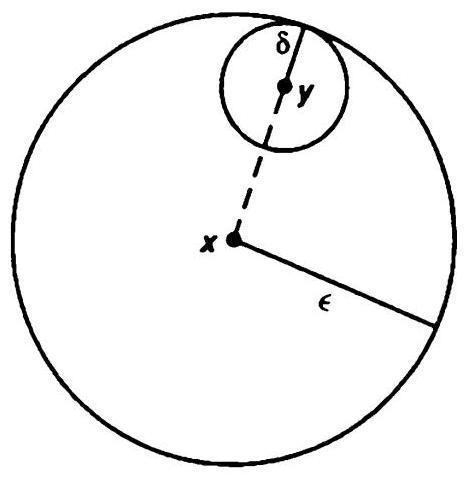
\includegraphics[width=0.4\textwidth]{images/20.1.jpg}
\end{center}
\hspace*{3em} 

Figure 20.1

A set \(U\) is open in the metric topology induced by \(d\) if and only if for each \(y \in  U\) , there is a \(\delta  > 0\) such that \({B}_{d}( {y,\delta })  \subset  U\) .

Clearly this condition implies that \(U\) is open. Conversely, if \(U\) is open, it contains a basis element \(B = {B}_{d}( {x,\epsilon })\) containing \(y\) , and \(B\) in turn contains a basis element \({B}_{d}( {y,\delta })\) centered at \(y\)

\begin{centeredblock}
\begin{example}
	Given a set \(X\) , define

\[
d( {x,y})  = 1\;\text{ if }x \neq  y,
\]

\[
d( {x,y})  = 0\;\text{ if }x = y
\]

It is trivial to check that \(d\) is a metric. The topology it induces is the discrete topology; the basis element \(B( {x,1})\) , for example, consists of the point \(x\) alone.
\end{example}
\end{centeredblock}

\begin{centeredblock}
\begin{example}
	The standard metric on the real numbers \(\mathbb{R}\) is defined by the equation

\[
d( {x,y})  = | {x - y}|
\]

It is easy to check that \(d\) is a metric. The topology it induces is the same as the order topology: Each basis element(a, b)for the order topology is a basis element for the metric topology, indeed,

\[
( {a,b})  = B( {x,\epsilon }) ,
\]

where \(x = ( {a + b}) /2\) and \(\epsilon  = ( {b - a}) /2\) . And conversely, each \(\epsilon\) -ball \(B( {x,\epsilon })\) equals an open interval the interval \(( {x - \epsilon ,x + \epsilon })\) .
\end{example}
\end{centeredblock}

\begin{definition}
	If \(X\) is a topological space, \(X\) is said to be metrizable if there exists a metric \(d\) on the set \(X\) that induces the topology of \(X\) . A metric space is a \index{metrizable space} \(X\) together with a specific metric \(d\) that gives the topology of \(X\) .
\end{definition}

Many of the spaces important for mathematics are metrizable, but some are not. Metrizability is always a highly desirable attribute for a space to possess, for the existence of a metric gives one a valuable tool for proving theorems about the space.

It is, therefore, a problem of fundamental importance in topology to find conditions on a topological space that will guarantee it is metrizable. One of our goals in Chapter 4 will be to find such conditions; they are expressed there in the famous theorem called Urysohn's metrization theorem. Further metrization theorems appear in Chapter 6. In the present section we shall content ourselves with proving merely that \({\mathbb{R}}^{n}\) and \({\mathbb{R}}^{\omega }\) are metrizable.

Although the \index{Product topology!metrizability}metrizability problem is an important problem in topology, the study \index{First-countability!of metric space}of metric spaces as such does not properly belong to topology as much as it does to analysis Metrzability of a space depends only on the topology of the space in question, but properties that involve a specific \index{Discrete topology!metric for}metric for \(X\) in general do not. For instance, one can make the following definition in a metric space.

\begin{definition}
	Let \(X\) be a metric space with metric \(d\) . A subset \(A\) of \(X\) is said to be \index{Bounded set} bounded if there is some number \(M\) such that

\[
d( {{a}_{1},{a}_{2}})  \leq  M
\]

for every pair \({a}_{1},{a}_{2}\) of points of \(A\) . If \(A\) is \index{Metric!bounded}bounded and nonempty, the \index{Diameter of a set} diameter of \(A\) is defined to be the number

\[
\operatorname{diam}A = \sup \{  {d( {{a}_{1},{a}_{2}})  \mid  {a}_{1},{a}_{2} \in  A}\}  .
\]
\end{definition}

Boundedness of a set is not a topological property, for it depends on the particular metric \(d\) that is used for \(X\) . For instance, if \(X\) is a metric space with metric \(d\) , then there exists a metric \(\bar{d}\) that gives the topology of \(X\) , relative to which every subset of \(X\) is bounded. It is defined as follows

\begin{theorem}
	Let \(X\) be a metric space with metric \(d\) . Define \(\index{d@\(\widetilde{d}\)} : X \times  X \rightarrow  \mathbb{R}\) by the equation

\[
\bar{d}( {x,y})  = \min \{ d( {x,y}) ,1\}
\]

Then \(\bar{d}\) is a metric that induces the same topology as \(d\) .

The metric \(\bar{d}\) is called the standard \index{bounded metric} corresponding to \(d\) .

\end{theorem}
\begin{proof}
Checking the first two conditions for a metric is trivial. Let us check the triangle inequality:

\[
\bar{d}( {x,z})  \leq  \bar{d}( {x,y})  + \bar{d}( {y,z}) .
\]

Now if either \(d( {x,y})  \geq  1\) or \(d( {y,z})  \geq  1\) , then the right side of this inequality is at least 1, since the left side is (by definition) at most 1, the inequality holds. It remains to consider the case in which \(d( {x,y})  < 1\) and \(d( {y,z})  < 1\) . In this case, we have

\[
d( {x,z})  \leq  d( {x,y})  + d( {y,z})  = \bar{d}( {x,y})  + \bar{d}( {y,z}) .
\]

Since \(\bar{d}( {x,z})  \leq  d( {x,z})\) by definition, the \index{Triangle inequality}triangle inequality holds for \(\bar{d}\) .

Now we note that in any metric space, the collection of \(\epsilon\) -balls with \(\epsilon  < 1\) forms a basis for the metric topology, for every basis element containing \(x\) contains such an \(\epsilon\) -ball centered at \(x\) . It follows that \(d\) and \(\bar{d}\) induce the same topology on \(X\) , because the collections of \(\epsilon\) -balls with \(\epsilon  < 1\) under these two metrics are the same collection.

Now we consider some familiar spaces and show they are metrizable.
\end{proof}

\begin{definition}
	Given \(\mathbf{x} = ( {{x}_{1},\ldots ,{x}_{n}})\) in \({\mathbb{R}}^{n}\) , we define the \index{norm} of \(\mathbf{x}\) by the equation

\[
\parallel x\parallel  = {( {x}_{1}^{2} + \cdots  + {x}_{n}^{2}) }^{1/2}
\]

and we define the \index{euclidean metric} \(d\) on \({\mathbb{R}}^{n}\) by the equation

\[
d( {\mathbf{x},\mathbf{y}})  = \parallel \mathbf{x} - \mathbf{y}\parallel  = {[  {( {x}_{1} - {y}_{1}) }^{2} + \cdots  + {( {x}_{n} - {y}_{n}) }^{2}]  }^{1/2}.
\]
\end{definition}

We define the square metric \(\index{rho@\(\rho\)}\) by the equation

\[
\rho ( {\mathbf{x},\mathbf{y}})  = \max \{  {| {{x}_{1} - {y}_{1}}| ,\ldots ,| {{x}_{n} - {y}_{n}}| }\}  .
\]

The proof that \(d\) is a metric requires some work; it is probably already familiar to you. If not, a proof is outlined in the exercises. We shall seldom have occasion to use this metric on \({\mathbb{R}}^{n}\)

To show that \(\rho\) is a metric is easier. Only the triangle inequality is nontrivial. From the triangle inequality for \(\mathbb{R}\) it follows that for each positive integer \(i\) ,

\[
| {{x}_{i} - {z}_{i}}|  \leq  | {{x}_{i} - {y}_{i}}|  + | {{y}_{i} - {z}_{i}}| .
\]

Then by definition of \(\rho\) ,

\[
| {{x}_{t} - {z}_{i}}|  \leq  \rho ( {\mathbf{x},\mathbf{y}})  + \rho ( {\mathbf{y},\mathbf{z}}) .
\]

As a result

\[
\rho ( {\mathbf{x},\mathbf{z}})  = \max \{  | {{x}_{i} - {z}_{i}}| \}   \leq  \rho ( {\mathbf{x},\mathbf{y}})  + \rho ( {\mathbf{y},\mathbf{z}}) ,
\]

as desired.

On the real line \(\mathbb{R} = {\mathbb{R}}^{1}\) , these two metrics coincide with the standard metric for \(\mathbb{R}\) . In the plane \({\mathbb{R}}^{2}\) , the basis elements under \(d\) can be pictured as circular regions, while the basis elements under \(\rho\) can be pictured as square regions.

We now show that each of these metrics induces the usual topology on \({\mathbb{R}}^{n}\) . We need the following lemma:

\begin{lemma}
	Let \(d\) and \({d}^{\prime }\) be two metrics on the set \(X\) ; let \(\mathcal{T}\) and \({\mathcal{T}}^{\prime }\) be the topologies they induce, respectively. Then \({\mathcal{T}}^{\prime }\) is finer than \(\mathcal{T}\) if and only if for each \(x\) in \(X\) and each \(\epsilon  > 0\) , there exists a \(\delta  > 0\) such that

\[
{B}_{{d}^{\prime }}( {x,\delta })  \subset  {B}_{d}( {x,\epsilon })
\]
\end{lemma}

\begin{proof}
Suppose that \({\mathcal{T}}^{\prime }\) is finer than \(\mathcal{T}\) Given the basis element \({B}_{d}( {x,\epsilon })\) for \(\mathcal{T}\) , there is by Lemma 13.3 a basis element \({B}^{\prime }\) for the topology \({\mathcal{T}}^{\prime }\) such that \(x \in  {B}^{\prime } \subset  {B}_{d}( {x,\epsilon })\) . Within \({B}^{\prime }\) we can find a ball \({B}_{{d}^{\prime }}( {x,\delta })\) centered at \(x\) .

Conversely, suppose the \(\delta\) - \(\epsilon\) condition holds Given a basis element \(B\) for \(\mathcal{T}\) containing \(x\) , we can find within \(B\) a ball \({B}_{d}( {x,\epsilon })\) centered at \(x\) . By the given condition, there is a \(\delta\) such that \({B}_{{d}^{\prime }}( {x,\delta })  \subset  {B}_{d}( {x,\epsilon })\) . Then Lemma 13.3 applies to show \({\mathcal{T}}^{\prime }\) is finer than \(\mathcal{T}\) .
\end{proof}

\begin{theorem}
	The topologies on \({\mathbb{R}}^{n}\) induced by the \index{Euclidean metric}euclidean metric \(d\) and the square metric \(\rho\) are the same as the product topology on \({\mathbb{R}}^{n}\) .

\end{theorem}
\begin{proof}
Let \(\mathbf{x} = ( {{x}_{1},\ldots ,{x}_{n}})\) and \(\mathbf{y} = ( {{y}_{1},\ldots ,{y}_{n}})\) be two points of \({\mathbb{R}}^{n}\) . It is simple algebra to check that

\[
\rho ( {\mathbf{x},\mathbf{y}})  \leq  d( {\mathbf{x},\mathbf{y}})  \leq  \sqrt{n}\rho ( {\mathbf{x},\mathbf{y}})
\]

The first inequality shows that

\[
{B}_{d}( {\mathbf{x},\epsilon })  \subset  {B}_{\rho }( {\mathbf{x},\epsilon })
\]

for all \(\mathbf{x}\) and \(\epsilon\) , since if \(d( {\mathbf{x},\mathbf{y}})  < \epsilon\) , then \(\rho ( {\mathbf{x},\mathbf{y}})  < \epsilon\) also. Similarly, the second inequality shows that

\[
{B}_{\rho }( {\mathbf{x},\epsilon /\sqrt{n}})  \subset  {B}_{d}( {\mathbf{x},\epsilon })
\]

for all \(x\) and \(\epsilon\) . It follows from the preceding lemma that the two metric topologies are the same.

Now we show that the product topology is the same as that given by the metric \(\rho\) . First, let

\[
B = ( {{a}_{1},{b}_{1}})  \times   \cdot   \times  ( {{a}_{n},{b}_{n}})
\]

be a basis element for the product topology, and let \(\mathbf{x} = ( {{x}_{1},\ldots ,{x}_{n}})\) be an element of \(B\) . For each \(i\) , there is an \({\epsilon }_{i}\) such that

\[
( {{x}_{l} - {\epsilon }_{i},{x}_{i} + {\epsilon }_{l}})  \subset  ( {{a}_{i},{b}_{i}}) ,
\]

choose \(\epsilon  = \min \{  {{\epsilon }_{1},\ldots ,{\epsilon }_{n}}\}\) . Then \({B}_{\rho }( {\mathbf{x},\epsilon })  \subset  B\) , as you can readily check. As a result, the \(\rho\) -topology is finer than the product topology.

Conversely, let \({B}_{\rho }( {\mathbf{x},\epsilon })\) be a basis element for the \(\rho\) -topology. Given the element \(\mathbf{y} \in  {B}_{\rho }( {\mathbf{x},\epsilon })\) , we need to find a basis element \(B\) for the product topology such that

\[
\mathbf{y} \in  B \subset  {B}_{\rho }( {\mathbf{x},\epsilon }) \text{ . }
\]

But this is trivial, for

\[
{B}_{\rho }( {\mathbf{x},\epsilon })  = ( {{x}_{1} - \epsilon ,{x}_{1} + \epsilon })  \times  \cdots  \times  ( {{x}_{n} - \epsilon ,{x}_{n} + \epsilon })
\]

is itself a basis element for the product topology.

Now we consider the infinite cartesian product \({\mathbb{R}}^{\omega }\) . It is natural to try to generalize the metrics \(d\) and \(\rho\) to this space. For instance, one can attempt to define a metric \(d\) on \({\mathbb{R}}^{\omega }\) by the equation

\[
d( {\mathbf{x},\mathbf{y}})  = {[  \mathop{\sum }\limits_{{i = 1}}^{\infty }{( {x}_{i} - {y}_{i}) }^{2}]  }^{1/2}.
\]

But this equation does not always make sense, for the series in question need not converge. (This equation does define a metric on a certain important subset of \({\mathbb{R}}^{\omega }\) , however; see the exercises.)

Similarly, one can attempt to generalize the square metric \(\rho\) to \({\mathbb{R}}^{\omega }\) by defining

\[
\rho ( {\mathbf{x},\mathbf{y}})  = \sup \{  | {{x}_{n} - {y}_{n}}| \}  .
\]

Again, this formula does not always make sense. If however we replace the usual metric \(d( {x,y})  = | {x - y}|\) on \(\mathbb{R}\) by its bounded counterpart \(d( {x,y})  = \min \{ | {x - y}| ,1\}\) , then this definition does make sense; it gives a metric on \({\mathbb{R}}^{\omega }\) called the uniform metric.

The uniform metric can be defined more generally on the cartesian product \({\mathbb{R}}^{J}\) for arbitrary \(J\) , as follows:
\end{proof}

\begin{definition}
	Given an index set \(J\) , and given points \(\mathbf{x} = {( {x}_{\alpha }) }_{\alpha  \in  J}\) and \(\mathbf{y} = {( {y}_{\alpha }) }_{\alpha  \in  J}\) of \({\mathbb{R}}^{J}\) , let us define a metric \(\bar{\rho }\) on \({\mathbb{R}}^{J}\) by the equation

\[
\bar{\rho }( {\mathbf{x},\mathbf{y}})  = \sup \{ \bar{d}( {{x}_{\alpha },{y}_{\alpha }})  \mid  \alpha  \in  J\} ,
\]

where \(\bar{d}\) is the \index{Standard bounded metric}standard bounded metric on \(\mathbb{R}\) . It is easy to check that \(\bar{\rho }\) is indeed a metric; it is called the uniform metric on \({\mathbb{R}}^{J}\) , and the topology it induces is called the uniform topology.
\end{definition}

The relation between this topology and the product and box topologies is the following:

\begin{theorem}
	The uniform topology on \({\mathbb{R}}^{J}\) is finer than the product topology and coarser than the box topology; these three topologies are all different if \(J\) is infinite.

\end{theorem}
\begin{proof}
Suppose that we are given a point \(\mathbf{x} = {( {x}_{\alpha }) }_{\alpha  \in  J}\) and a product topology basis element \(\prod {U}_{\alpha }\) about \(\mathbf{x}\) . Let \({\alpha }_{1},\ldots ,{\alpha }_{n}\) be the indices for which \({U}_{\alpha } \neq  \mathbb{R}\) . Then for each \(i\) , choose \({\epsilon }_{i} > 0\) so that the \({\epsilon }_{i}\) -ball centered at \({x}_{{\alpha }_{i}}\) in the \(d\) metric is contained in \({U}_{{\alpha }_{i}}\) ; this we can do because \({U}_{{\alpha }_{i}}\) is open in \(\mathbb{R}\) . Let \(\epsilon  = \min \{  {{\epsilon }_{1},\ldots ,{\epsilon }_{n}}\}\) ; then the \(\epsilon\) -ball centered at \(\mathbf{x}\) in the \(\bar{\rho }\) metric is contained in \(\prod {U}_{\alpha }\) . For if \(\mathbf{z}\) is a point of \({\mathbb{R}}^{J}\) such that \(\widetilde{\rho }( {\mathbf{x},\mathbf{z}})  < \epsilon\) , then \(\widetilde{d}( {{x}_{\alpha },{z}_{\alpha }})  < \epsilon\) for all \(\alpha\) , so that \(\mathbf{z} \in  \prod {U}_{\alpha }\) . It follows that the uniform topology is finer than the product topology.

On the other hand, let \(B\) be the \(\epsilon\) -ball centered at \(\mathbf{x}\) in the \(\bar{\rho }\) metric. Then the box neighborhood

\[
U = \prod ( {{x}_{\alpha } - \frac{1}{2}\epsilon ,{x}_{\alpha } + \frac{1}{2}\epsilon })
\]

of \(\mathbf{x}\) is contained in \(B\) . For if \(\mathbf{y} \in  U\) , then \(\bar{d}( {{x}_{\alpha },{y}_{\alpha }})  < \frac{1}{2}\epsilon\) for all \(\alpha\) , so that \(\bar{\rho }( {\mathbf{x},\mathbf{y}})  \leq\)  \(\frac{1}{2}\epsilon\) .

Showing these three topologies are different if \(J\) is infinite is a task we leave to the exercises.

In the case where \(J\) is infinite, we still have not determined whether \({\mathbb{R}}^{J}\) is metrizable in either the box or the product topology. It turns out that the only one of these cases where \({\mathbb{R}}^{J}\) is metrizable is the case where \(J\) is countable and \({\mathbb{R}}^{J}\) has the product topology. As we shall see.
\end{proof}

\begin{theorem}
	Let \(\bar{d}( {a,b})  = \min \{ | {a - b}| ,1\}\) be the standard bounded metric on \(\mathbb{R}\) . If \(\mathbf{x}\) and \(\mathbf{y}\) are two points of \({\mathbb{R}}^{\omega }\) , define

\[
D( {\mathbf{x},\mathbf{y}})  = \sup \{  \frac{\bar{d}( {{x}_{i},{y}_{i}}) }{i}\}  .
\]

Then \(D\) is a metric that induces the product topology on \({\mathbb{R}}^{\omega }\) .

\end{theorem}
\begin{proof}
The properties of a metric are satisfied trivially except for the triangle inequality, which is proved by noting that for all \(i\) ,

\[
\frac{\bar{d}( {{x}_{i},{z}_{l}}) }{i} \leq  \frac{\bar{d}( {{x}_{l},{y}_{i}}) }{i} + \frac{\bar{d}( {{y}_{l},{z}_{i}}) }{i} \leq  D( {\mathbf{x},\mathbf{y}})  + D( {\mathbf{y},\mathbf{z}}) ,
\]

so that

\[
\sup \{  \frac{\bar{d}( {{x}_{i},{z}_{i}}) }{i}\}   \leq  D( {\mathbf{x},\mathbf{y}})  + D( {\mathbf{y},\mathbf{z}}) .
\]

The fact that \(D\) gives the product topology requires a \index{Little ell-two topology} little more work. First, let \(U\) be open in the metric topology and let \(\mathbf{x} \in  U\) ; we'find an open set \(V\) in the product topology such that \(\mathbf{x} \in  V \subset  U\) . Choose an \(\epsilon\) -ball \({B}_{D}( {\mathbf{x},\epsilon })\) lying in \(U\) . Then choose \(N\) large enough that \(1/N < \epsilon\) . Finally, let \(V\) be the basis element for the product topology

\[
V = ( {{x}_{1} - \epsilon ,{x}_{1} + \epsilon })  \times  \cdots  \times  ( {{x}_{N} - \epsilon ,{x}_{N} + \epsilon })  \times  \mathbb{R} \times  \mathbb{R} \times  \cdots .
\]

We assert that \(V \subset  {B}_{D}( {\mathbf{x},\epsilon })\) : Given any \(\mathbf{y}\) in \({\mathbb{R}}^{\omega }\) ,

\[
\frac{\bar{d}( {{x}_{i},{y}_{i}}) }{i} \leq  \frac{1}{N}\;\text{ for }i \geq  N.
\]

Therefore,

\[
D( {\mathbf{x},\mathbf{y}})  \leq  \max \{  {\frac{\bar{d}( {{x}_{1},{y}_{1}}) }{1},\cdots ,\frac{\bar{d}( {{x}_{N},{y}_{N}}) }{N},\frac{1}{N}}\}  .
\]

If \(\mathbf{y}\) is in \(V\) , this expression is less than \(\epsilon\) , so that \(V \subset  {B}_{D}( {\mathbf{x},\epsilon })\) , as desired.

Conversely, consider a basis element

\[
U = \mathop{\prod }\limits_{{i \in  {\mathbb{Z}}_{ + }}}{U}_{i}
\]

for the product topology, where \({U}_{i}\) is open in \(\mathbb{R}\) for \(i = {\alpha }_{1},\ldots ,{\alpha }_{n}\) and \({U}_{i} = \mathbb{R}\) for all other indices i. Given \(\mathbf{x} \in  U\) , we find an open set \(V\) of the metric topology such that \(\mathbf{x} \in  V \subset  U\) . Choose an interval \(( {{x}_{t} - {\epsilon }_{i},{x}_{i} + {\epsilon }_{i}})\) in \(\mathbb{R}\) centered about \({x}_{t}\) and lying in \({U}_{i}\) for \(i = {\alpha }_{1},\ldots ,{\alpha }_{n}\) ; choose each \({\epsilon }_{i} \leq  1\) . Then define

\[
\epsilon  = \min \{  {{\epsilon }_{i}/\mathrm{i} \mid  \mathrm{i} = {\alpha }_{1},\ldots ,{\alpha }_{n}}\}  .
\]

We assert that

\[
\mathbf{x} \in  {B}_{D}( {\mathbf{x},\epsilon })  \subset  U\text{ . }
\]

Let \(\mathbf{y}\) be a point of \({B}_{D}( {\mathbf{x},\epsilon })\) . Then for all \(i\) ,

\[
\frac{\bar{d}( {{x}_{i},{y}_{i}}) }{\mathrm{i}} \leq  D( {\mathbf{x},\mathbf{y}})  < \epsilon .
\]

Now if \(i = {\alpha }_{1},\ldots ,{\alpha }_{n}\) , then \(\epsilon  \leq  {\epsilon }_{i}/i\) , so that \(\widetilde{d}( {{x}_{i},{y}_{i}})  < {\epsilon }_{i} \leq  1\) ; it follows that \(| {{x}_{i} - {y}_{i}}|  < {\epsilon }_{i}\) . Therefore, \(\mathbf{y} \in  \prod {U}_{i}\) , as desired.
\end{proof}

\section*{Exercises}
\begin{enumerate}[itemsep=0.4em, parsep=0pt, topsep=0pt, partopsep=0pt, leftmargin=*, label=\arabic*., ref=\arabic*]
\item
  \begin{enumerate}[itemsep=0.2em, parsep=0pt, topsep=0pt, partopsep=0pt, leftmargin=*, label=(\alph*), align=left]
  \item In \({\mathbb{R}}^{n}\) , define \[ {d}^{\prime }( {\mathbf{x},\mathbf{y}})  = | {{x}_{1} - {y}_{1}}|  + \cdots  + | {{x}_{n} - {y}_{n}}| . \] Show that \({d}^{\prime }\) is a metric that induces the usual topology of \({\mathbb{R}}^{n}\) . Sketch the basis elements under \({d}^{\prime }\) when \(n = 2\) .

  \item More generally, given \(p \geq  1\) , define \[ {d}^{\prime }( {\mathbf{x},\mathbf{y}})  = {[  \mathop{\sum }\limits_{{i = 1}}^{n}{| {x}_{i} - {y}_{i}| }^{p}]  }^{1/p} \] for \(\mathbf{x},\mathbf{y} \in  {\mathbb{R}}^{n}\) . Assume that \({d}^{\prime }\) is a metric. Show that it induces the usual topology on \({\mathbb{R}}^{n}\) .
  \end{enumerate}
\item Show that \(\mathbb{R} \times  \mathbb{R}\) in the dictionary order topology is metrizable.
\item Let \(X\) be a metric space with metric \(d\) .
  \begin{enumerate}[itemsep=0.2em, parsep=0pt, topsep=0pt, partopsep=0pt, leftmargin=*, label=(\alph*), align=left]
  \item Show that \(d : X \times  X \rightarrow  \mathbb{R}\) is continuous.
  \item Let \({X}^{\prime }\) denote a space having the same underlying set as \(X\) . Show that if \(d : {X}^{\prime } \times  {X}^{\prime } \rightarrow  \mathbb{R}\) is continuous, then the topology of \({X}^{\prime }\) is finer than the topology of \(X\) . One can summarize the result of this exercise as follows: If \(X\) has a metric \(d\) , then the topology induced by \(d\) is the coarsest topology relative to which the function \(d\) is continuous. 4. Consider the product, uniform, and box topologies on \({\mathbb{R}}^{\omega }\) .
  \item In which topologies are the following functions from \(\mathbb{R}\) to \({\mathbb{R}}^{\omega }\) continuous? \[ f( t)  = ( {t,{2t},{3t},\ldots }) , \] \[ g( t)  = ( {t,t,t,\ldots }) , \] \[ h( t)  = ( {t,\frac{1}{2}t,\frac{1}{3}t,\ldots }) . \]
  \item In which topologies do the following sequences converge? \[ {\mathbf{w}}_{1} = ( {1,1,1,1,\ldots }) ,\;{\mathbf{x}}_{1} = ( {1,1,1,1,\ldots }) , \] \[ {\mathbf{w}}_{2} = ( {0,2,2,2,\ldots }) ,\;{\mathbf{x}}_{2} = ( {0,\frac{1}{2},\frac{1}{2},\frac{1}{2},\ldots }) , \] \[ {\mathbf{w}}_{3} = ( {0,0,3,3,\ldots }) ,\;{\mathbf{x}}_{3} = ( {0,0,\frac{1}{3},\frac{1}{3}\ldots }) , \] ... ... \[ {\mathbf{y}}_{1} = ( {1,0,0,0,\ldots }) ,\;{\mathbf{z}}_{1} = ( {1,1,0,0,\ldots }) , \] \[ {\mathbf{y}}_{2} = ( {\frac{1}{2},\frac{1}{2},0,0,\ldots }) ,\;{\mathbf{z}}_{2} = ( {\frac{1}{2},\frac{1}{2},0,0,\ldots }) , \] \[ {\mathbf{y}}_{3} = ( {\frac{1}{3},\frac{1}{3},\frac{1}{3},0,\ldots }) ,\;{\mathbf{z}}_{3} = ( {\frac{1}{3},\frac{1}{3},0,0,\ldots }) , \] ... ...
  \end{enumerate}
\item Let \({\mathbb{R}}^{\infty }\) be the subset of \({\mathbb{R}}^{\omega }\) consisting of all sequences that are eventually zero. What is the closure of \({\mathbb{R}}^{\infty }\) in \({\mathbb{R}}^{\omega }\) in the uniform topology? Justify your answer.
\item Let \(\bar{\rho }\) be the uniform metric on \({\mathbb{R}}^{\omega }\) . Given \(\mathbf{x} = ( {{x}_{1},{x}_{2},\ldots })  \in  {\mathbb{R}}^{\omega }\) and given \(0 < \epsilon  < 1\) , let \[ U( {\mathbf{x},\epsilon })  = ( {{x}_{1} - \epsilon ,{x}_{1} + \epsilon })  \times  \cdots  \times  ( {{x}_{n} - \epsilon ,{x}_{n} + \epsilon })  \times  \cdots . \]
  \begin{enumerate}[itemsep=0.2em, parsep=0pt, topsep=0pt, partopsep=0pt, leftmargin=*, label=(\alph*), align=left]
  \item Show that \(U( {\mathbf{x},\epsilon })\) is not equal to the \(\epsilon\) -ball \({B}_{\bar{\rho }}( {\mathbf{x},\epsilon })\) .
  \item Show that \(U( {\mathbf{x},\epsilon })\) is not even open in the uniform topology.
  \item Show that \[ {B}_{\bar{\rho }}( {\mathbf{x},\epsilon })  = \mathop{\bigcup }\limits_{{\delta  < \epsilon }}U( {\mathbf{x},\delta }) . \]
  \end{enumerate}
\item Consider the map \(h : {\mathbb{R}}^{\omega } \rightarrow  {\mathbb{R}}^{\omega }\) defined in Exercise 8 of \(§{19}\) , give \({\mathbb{R}}^{\omega }\) the uniform topology. Under what conditions on the numbers \({a}_{i}\) and \({b}_{i}\) is \(h\) continuous? a homeomorphism?
\item Let \(X\) be the subset of \({\mathbb{R}}^{\omega }\) consisting of all sequences \(\mathbf{x}\) such that \(\sum {x}_{i}^{2}\) converges. Then the formula \[ d( {\mathbf{x},\mathbf{y}})  = {[  \mathop{\sum }\limits_{{i = 1}}^{\infty }{( {x}_{i} - {y}_{i}) }^{2}]  }^{1/2} \] defines a metric on \(X\) . (See Exercise 10.) On \(X\) we have the three topologies it inherits from the box, uniform, and product topologies on \({\mathbb{R}}^{\omega }\) . We have also the topology given by the metric \(d\) , which we call the \({\ell }^{2}\) -topology. (Read ``little ell two.'')
  \begin{enumerate}[itemsep=0.2em, parsep=0pt, topsep=0pt, partopsep=0pt, leftmargin=*, label=(\alph*), align=left]
  \item Show that on \(X\) , we have the inclusions \[ \text{ box topology } \supset  {\ell }^{2}\text{ -topology } \supset  \text{ uniform topology. } \]
  \item The set \({\mathbb{R}}^{\infty }\) of all sequences that are eventually zero is contained in \(X\) . Show that the four topologies that \({\mathbb{R}}^{\infty }\) inherits as a subspace of \(X\) are all distinct.
  \item The set \[ H = \mathop{\prod }\limits_{{n \in  {\mathbb{Z}}_{ + }}}[  {0,1/n}] \] is contained in \(X\) , it is called the \index{Hilbert cube}. Compare the four topologies that \(H\) inherits as a subspace of \(X\) .
  \end{enumerate}
\item Show that the euclidean metric \(d\) on \({\mathbb{R}}^{n}\) is a metric, as follows: If \(\mathbf{x},\mathbf{y} \in  {\mathbb{R}}^{n}\) and \(c \in  \mathbb{R}\) , define \[ \mathbf{x} + \mathbf{y} = ( {{x}_{1} + {y}_{1},\ldots ,{x}_{n} + {y}_{n}}) , \] \[ c\mathbf{x} = ( {c{x}_{1},\ldots ,c{x}_{n}}) , \] \[ \mathbf{x} \cdot  \mathbf{y} = {x}_{1}{y}_{1} + \cdots  + {x}_{n}{y}_{n} \]
  \begin{enumerate}[itemsep=0.2em, parsep=0pt, topsep=0pt, partopsep=0pt, leftmargin=*, label=(\alph*), align=left]
  \item Show that \(\mathbf{x} \cdot  ( {\mathbf{y} + \mathbf{z}})  = ( \begin{array}{ll} \mathbf{x} & \mathbf{y} \end{array})  + ( {\mathbf{x} \cdot  \mathbf{z}})\) .
  \item Show that \(| {\mathbf{x} \cdot  \mathbf{y}}|  \leq  \parallel \mathbf{x}\parallel \parallel \mathbf{y}\parallel\) . [Hint: If \(\mathbf{x},\mathbf{y} \neq  0\) , let \(a = 1/\parallel \mathbf{x}\parallel\) and \(b = 1/\parallel \mathbf{y}\parallel\) , and use the fact that \(\parallel {ax} \pm  {by}\parallel  \geq  0\) .\}
  \item Show that \(\parallel \mathbf{x} + \mathbf{y}\parallel  \leq  \parallel \mathbf{x}\parallel  + \parallel \mathbf{y}\parallel\) . [Hint: Compute \(( {\mathbf{x} + \mathbf{y}})  \cdot  ( {\mathbf{x} + \mathbf{y}})\) and apply (b).\}
  \item Verify that \(d\) is a metric.
  \end{enumerate}
\item Let \(X\) denote the subset of \({\mathbb{R}}^{\omega }\) consisting of all sequences \(( {{x}_{1},{x}_{2},\ldots })\) such that \(\sum {x}_{i}^{2}\) converges. (You may assume the standard facts about infinite series. In case they are not familiar to you, we shall give them in Exercise 11 of the next section.)
  \begin{enumerate}[itemsep=0.2em, parsep=0pt, topsep=0pt, partopsep=0pt, leftmargin=*, label=(\alph*), align=left]
  \item Show that if \(x,y \in  X\) , then \(\sum | {{x}_{i}{y}_{i}}|\) converges. [Hint: Use (b) of Exercise 9 to show that the partial sums are bounded.\}
  \item Let \(c \in  \mathbb{R}\) . Show that if \(x,y \in  X\) , then so are \(x + y\) and \({cx}\) .
  \item Show that \[ d( {\mathbf{x},\mathbf{y}})  = {[  \mathop{\sum }\limits_{{i = 1}}^{\infty }{( {x}_{i} - {y}_{i}) }^{2}]  }^{1/2} \] is a well-defined metric on \(X\) . *11. Show that if \(d\) is a metric for \(X\) , then \[ {d}^{\prime }( {x,y})  = d( {x,y}) /( {1 + d( {x,y}) }) \] is a bounded metric that gives the topology of \(X\) . [Hint: If \(f( x)  = x/( {1 + x})\) for \(x > 0\) , use the mean-value theorem to show that \(f( {a + b})  - f( b)  \leq  {f}^{\prime }( a)\) .]
  \end{enumerate}
\end{enumerate}
\section*{§ 21 The Metric Topology (continued)}

In this section, we discuss the relation of the metric topology to the concepts we have previously introduced.

Subspaces of metric spaces behave the way one would wish them to, if \(A\) is a subspace of the topological space \(X\) and \(d\) is a metric for \(X\) , then the restriction of \(d\) to \(A \times  A\) is a metric for the topology of \(A\) . This we leave to you to check.

About order topologies there is nothing to be said; some are metrizable (for instance, \({\mathbb{Z}}_{ + }\) and \(\mathbb{R}\) ), and others are not, as we shall see

The Hausdorff axiom is satisfied by every metric topology. If \(x\) and \(y\) are distinct points of the metric space(X, d), we let \(\epsilon  = \frac{1}{2}d( {x,y})\) ; then the triangle inequality implies that \({B}_{d}( {x,\epsilon })\) and \({B}_{d}( {y,\epsilon })\) are disjoint.

The product topology we have already considered in special cases; we have proved that the products \({\mathbb{R}}^{n}\) and \({\mathbb{R}}^{\omega }\) are metrizable. It is true in general that countable products of \index{Metrizable space}metrizable spaces are metrizable; the proof follows a pattern similar to the proof for \({\mathbb{R}}^{\omega }\) , so we leave it to the exercises.

About continuous functions there is a good deal to be said. Consideration of this topic will occupy the remainder of the section.

When we study continuous functions on metric spaces, we are about as close to the study of calculus and analysis as we shall come in this book. There are two things we want to do at this point.

First, we want to show that the familiar `` \(\epsilon  - \delta\) definition'' of continuity carries over to general metric spaces, and so does the ``\index{Convergent sequence}convergent sequence definition'' of continuity.

Second, we want to consider two additional methods for constructing continuous functions, besides those discussed in §18. One is the process of taking sums, differences, products, and quotients of continuous real-valued functions. The other is the process of taking limits of uniformly \index{Product topology!convergent sequences}convergent sequences of continuous functions.

\begin{theorem}
	Let \(f : X \rightarrow  Y\) ; let \(X\) and \(Y\) be metrizable with metrics \({d}_{X}\) and \({d}_{Y}\) , respectively. Then continuity of \(f\) is equivalent to the requirement that given \(x \in  X\) and given \(\epsilon  > 0\) , there exists \(\delta  > 0\) such that

\[
{d}_{X}( {x,y})  < \delta  \Rightarrow  {d}_{Y}( {f( x) ,f( y) })  < \epsilon .
\]

\end{theorem}
\begin{proof}
Suppose that \(f\) is continuous. Given \(x\) and \(\epsilon\) , consider the set

\[
{f}^{-1}( {B( {f( x) ,\epsilon }) }) ,
\]

which is open in \(X\) and contains the point \(x\) . It contains some \(\delta\) -ball \(B( {x,\delta })\) centered at \(x\) . If \(y\) is in this \(\delta\) -ball, then \(f( y)\) is in the \(\epsilon\) -ball centered at \(f( x)\) , as desired.

Conversely, suppose that the \(\epsilon  - \delta\) condition is satisfied. Let \(V\) be open in \(Y\) ; we show that \({f}^{-1}( V)\) is open in \(X\) . Let \(x\) be a point of the set \({f}^{-1}( V)\) . Since \(f( x)  \in\)  \(V\) , there is an \(\epsilon\) -ball \(B( {f( x) ,\epsilon })\) centered at \(f( x)\) and contained in \(V\) . By the \(\epsilon\) - \(\delta\) condition, there is a \(\delta\) -ball \(B( {x,\delta })\) centered at \(x\) such that \(f( {B( {x,\delta }) })  \subset  B( {f( x) ,\epsilon })\) . Then \(B( {x,\delta })\) is a neighborhood of \(x\) contained in \({f}^{-1}( V)\) , so that \({f}^{-1}( V)\) is open, as desired.

Now we turn to the convergent sequence definition of continuity. We begin by considering the relation between convergent sequences \index{Sequences!and closure}and closures of sets. It is certainly believable, from one's experience in analysis, that if \(x\) lies in the closure of a subset \(A\) of the space \(X\) , then there should exist a sequence of points of \(A\) converging to \(x\) . This is not true in general, but it is true for metrizable spaces.
\end{proof}

\begin{lemma}[The \index{sequence lemma}]
	Let \(X\) be a topological space; let \(A \subset  X\) . If there is a sequence of points of \(A\) converging to \(x\) , then \(x \in  \bar{A}\) ; the converse holds if \(X\) is metrizable.
\end{lemma}

\begin{proof}
Suppose that \({x}_{n} \rightarrow  x\) , where \({x}_{n} \in  A\) . Then every neighborhood \(U\) of \(x\) contains a point of \(A\) , so \(x \in  \bar{A}\) by Theorem 17.5. Conversely, suppose that \(X\) is metrizable and \(x \in  \bar{A}\) . Let \(d\) be a metric for the topology of \(X\) . For each positive integer \(n\) , take the neighborhood \({B}_{d}( {x,1/n})\) of radius \(1/n\) of \(x\) , and choose \({x}_{n}\) to be a point of its intersection with \(A\) . We assert that the sequence \({x}_{n}\) converges to \(x\) : Any open set \(U\) containing \(x\) contains an \(\epsilon\) -ball \({B}_{d}( {x,\epsilon })\) centered at \(x\) ; if we choose \(N\) so that \(1/N < \epsilon\) , then \(U\) contains \({x}_{i}\) for all \(i \geq  N\) .
\end{proof}

\begin{theorem}
	Let \(f : X \rightarrow  Y\) . If the function \(f\) is continuous, then for every convergent sequence \({x}_{n} \rightarrow  x\) in \(X\) , the sequence \(f( {x}_{n})\) converges to \(f( x)\) . The converse holds if \(X\) is metrizable.

\end{theorem}
\begin{proof}
Assume that \(f\) is continuous. Given \({x}_{n} \rightarrow  x\) , we wish to show that \(f( {x}_{n})  \rightarrow\)  \(f( x)\) . Let \(V\) be a neighborhood of \(f( x)\) . Then \({f}^{-1}( V)\) is a neighborhood of \(x\) , and so there is an \(N\) such that \({x}_{n} \in  {f}^{-1}( V)\) for \(n \geq  N\) . Then \(f( {x}_{n})  \in  V\) for \(n \geq  N\) .

To prove the converse, assume that the convergent sequence condition is satisfied. Let \(A\) be a subset of \(X\) ; we show that \(f( \bar{A})  \subset  \overline{f( A) }\) . If \(x \in  \bar{A}\) , then there is a sequence \({x}_{n}\) of points of \(A\) converging to \(x\) (by the preceding lemma). By assumption, the sequence \(f( {x}_{n})\) converges to \(f( x)\) . Since \(f( {x}_{n})  \in  f( A)\) , the preceding lemma implies that \(f( x)  \in  \overline{f( A) }\) . (Note that metrizability of \(Y\) is not needed.) Hence \(f( \bar{A})  \subset\)  \(\overline{f( A) }\) , as desired.

Incidentally, in proving Lemma 21.2 and Theorem 213 we did not use the full strength of the hypothesis that the space \(X\) is metrizable. All we really needed was the countable collection \({B}_{d}( {x,1/n})\) of balls about \(x\) . This fact leads us to make a new definition

A space \(X\) is said to have a countable basis at the point \(x\) if there is a countable collection \({\{  {U}_{n}\}  }_{n \in  {\mathbb{Z}}_{ + }}\) of neighborhoods of \(x\) such that any neighborhood \(U\) of \(x\) contains at least one of the sets \({U}_{n}\) . A space \(X\) that has a countable basis at each of its points is said to satisfy the first countability axiom.

If \(X\) has a countable basis \(\{  {U}_{n}\}\) at \(x\) , then the proof of Lemma 212 goes through, one simply replaces the ball \({B}_{d}( {x,1/n})\) throughout by the set

\[
{B}_{n} = {U}_{1} \cap  {U}_{2} \cap   \cdot   \cdot   \cap  {U}_{n}.
\]

The proof of Theorem 213 goes through unchanged

A metrizable space always satisfies the first countability axiom, but the converse is not true, as we shall see. Like the Hausdorff axiom, the first countability axiom is a requirement that we sometimes impose on a topological space in order to prove stronger theorems about the space. We shall study it in more detail in Chapter 4

Now we consider additional methods for constructing continuous functions. We need the following lemma:
\end{proof}

\begin{lemma}
	The addition, subtraction, and multiplication operations are continuous functions from \(\mathbb{R} \times  \mathbb{R}\) into \(\mathbb{R}\) ; and the quotient operation is a continuous function from \(\mathbb{R} \times  ( {\mathbb{R}-\{ 0\} })\) into \(\mathbb{R}\) .
\end{lemma}

You have probably seen this lemma proved before; it is a standard `` \(\epsilon  - \delta\) argument.'' If not, a proof is outlined in Exercise 12 below; you should have no trouble filling in the details.

\begin{theorem}
	If \(X\) is a topological space, and if \(f,g : X \rightarrow  \mathbb{R}\) are continuous functions, then \(f + g,f - g\) , and \(f \cdot  g\) are continuous. If \(g( x)  \neq  0\) for all \(x\) , then \(f/g\) is continuous.

\end{theorem}
\begin{proof}
The map \(h : X \rightarrow  \mathbb{R} \times  \mathbb{R}\) defined by

\[
h( x)  = f( x)  \times  g( x)
\]

is continuous, by Theorem 18.4. The function \(f + g\) equals the composite of \(h\) and the addition operation

\[
+  : \mathbb{R} \times  \mathbb{R} \rightarrow  \mathbb{R}
\]

therefore \(f + g\) is continuous. Similar arguments apply to \(f - g,f \cdot  g\) , and \(f/g\) .

Finally, we come to the notion of \index{uniform convergence}.
\end{proof}

\begin{definition}
	Let \({f}_{n} : X \rightarrow  Y\) be a sequence of functions from the set \(X\) to the metric space \(Y\) . Let \(d\) be the metric for \(Y\) . We say that the sequence \(( {f}_{n})\) \index{Converges uniformly}converges uniformly to the function \(f : X \rightarrow  Y\) if given \(\epsilon  > 0\) , there exists an integer \(N\) such that

\[
d( {{f}_{n}( x) ,f( x) })  < \epsilon
\]

for all \(n > N\) and all \(x\) in \(X\) .
\end{definition}

Uniformity of convergence depends not only on the topology of \(Y\) but also on its metric. We have the following theorem about uniformly convergent sequences:

\begin{theorem}[Uniform limit theorem]
	Let \({f}_{n} : X \rightarrow  Y\) be a sequence of continuous functions from the topological space \(X\) to the metric space \(Y\) . If \(( {f}_{n})\) converges uniformly to \(f\) , then \(f\) is continuous.

\end{theorem}
\begin{proof}
Let \(V\) be open in \(Y\) ; let \({x}_{0}\) be a point of \({f}^{-1}( V)\) . We wish to find a neighborhood \(U\) of \({x}_{0}\) such that \(f( U)  \subset  V\) .

Let \({y}_{0} = f( {x}_{0})\) . First choose \(\epsilon\) so that the \(\epsilon\) -ball \(B( {{y}_{0},\epsilon })\) is contained in \(V\) . Then, using \index{Uniform convergence}uniform convergence, choose \(N\) so that for all \(n \geq  N\) and all \(x \in  X\) ,

\[
d( {{f}_{n}( x) ,f( x) })  < \epsilon /3\text{ . }
\]

Finally, using continuity of \({f}_{N}\) , choose a neighborhood \(U\) of \({x}_{0}\) such that \({f}_{N}\) carries \(U\) into the \(\epsilon /3\) ball in \(Y\) centered at \({f}_{N}( {x}_{0})\) .

We claim that \(f\) carries \(U\) into \(B( {{y}_{0},\epsilon })\) and hence into \(V\) , as desired. For this purpose, note that if \(x \in  U\) , then

\[
d( {f( x) ,{f}_{N}( x) })  < \epsilon /3\;\text{ (by choice of }N\text{ ), }
\]

\[
d( {{f}_{N}( x) ,{f}_{N}( {x}_{0}) })  < \epsilon /3\;\text{ (by choice of }U\text{ ), }
\]

\[
d( {{f}_{N}( {x}_{0}) ,f( {x}_{0}) })  < \epsilon /3\;\text{ (by choice of }N\text{ ). }
\]

Adding and using the triangle inequality, we see that \(d( {f( x) ,f( {x}_{0}) })  < \epsilon\) , as desired.

Let us remark that the notion of uniform convergence is related to the definition of the uniform metric, which we gave in the preceding section. Consider, for example, the space \({\mathbb{R}}^{X}\) of all functions \(f : X \rightarrow  \mathbb{R}\) , in the uniform metric \(\bar{\rho }\) . It is not difficult to see that a sequence of functions \({f}_{n} : X \rightarrow  \mathbb{R}\) converges uniformly to \(f\) if and only if the sequence \(( {f}_{n})\) converges to \(f\) when they are considered as elements of the metric space \(( {{\mathbb{R}}^{X},\bar{\rho }})\) . We leave the proof to the exercises.

We conclude the section with some examples of spaces that are not metrizable.
\end{proof}

\begin{centeredblock}
\begin{example}
	\({\mathbb{R}}^{\omega }\) in the box topology is not metrizable.

We shall show that the \index{Sequence lemma}sequence lemma does not hold for \({\mathbb{R}}^{\omega }\) . Let \(A\) be the subset of \({\mathbb{R}}^{\omega }\) consisting of those points all of whose coordinates are positive:

\[
A = \{  {( {{x}_{1},{x}_{2},\ldots })  \mid  {x}_{i} > 0\text{ for all }i \in  {\mathbb{Z}}_{ + }}\}  .
\]

Let0be the ``origin'' in \({\mathbb{R}}^{\omega }\) , that is, the point(0,0,.)each of whose coordinates is zero. In the box topology,0belongs to \(A\) ; for if

\[
B = ( {{a}_{1},{b}_{1}})  \times  ( {{a}_{2},{b}_{2}})  \times
\]

is any basis element containing0, then \(B\) intersects \(A\) . For instance, the point

\[
( {\frac{1}{2}{b}_{1},\frac{1}{2}{b}_{2}\ldots })
\]

belongs to \(B \cap  A\) .

But we assert that there is no sequence of points of \(A\) converging to0. For let \(( {\mathbf{a}}_{n})\) be a sequence of points of \(A\) , where

\[
{\mathbf{a}}_{n} = ( {{x}_{1n},{x}_{2n},\ldots ,{x}_{tn},\ldots }) .
\]

Every coordinate \({x}_{tn}\) is positive, so we can construct a basis element \({B}^{\prime }\) for the box topology on \(\mathbb{R}\) by setting

\[
{B}^{\prime } = ( {-{x}_{11},{x}_{11}})  \times  ( {-{x}_{22},{x}_{22}})  \times  .
\]

Then \({B}^{\prime }\) contains the origin0, but it contains no member of the sequence \(( {\mathbf{a}}_{n})\) ; the point \({a}_{n}\) cannot belong to \({B}^{\prime }\) because its \(n\) th coordinate \({x}_{nn}\) does not belong to the interval \(( {-{x}_{nn},{x}_{nn}})\) . Hence the sequence \(( {a}_{n})\) cannot converge to 0 in the box topology.
\end{example}
\end{centeredblock}

\begin{centeredblock}
\begin{example}
	An uncountable product of \(\mathbb{R}\) with itself is not metrizable.

Let \(J\) be an uncountable index set; we show that \({\mathbb{R}}^{J}\) does not satisfy the sequence lemma (in the product topology)

Let \(A\) be the subset of \({\mathbb{R}}^{J}\) consisting of all points \(( {x}_{\alpha })\) such that \({x}_{\alpha } = 1\) for all but finitely many values of \(\alpha\) Let 0 be the ``origin'' in \({\mathbb{R}}^{J}\) , the point each of whose coordinates is 0 .

We assert that0belongs to the closure of \(A\) Let \(\prod {U}_{\alpha }\) be a basis element containing0. Then \({U}_{\alpha } \neq  \mathbb{R}\) for only finitely many values of \(\alpha\) , say for \(\alpha  = {\alpha }_{1},\ldots {\alpha }_{n}\) . Let \(( {x}_{\alpha })\) be the point of \(A\) defined by letting \({x}_{\alpha } = 0\) for \(\alpha  = {\alpha }_{1},\ldots ,{\alpha }_{n}\) and \({x}_{\alpha } = 1\) for all other values of \(\alpha\) , then \(( {x}_{\alpha })  \in  A \cap  \prod {U}_{\alpha }\) , as desired.

But there is no sequence of points of \(A\) converging to0. For let \({\mathbf{a}}_{n}\) be a sequence of points of \(A\) . Given \(n\) , let \({J}_{n}\) denote the subset of \(J\) consisting of those indices \(\alpha\) for which the \(\alpha\) th coordinate of \({\mathbf{a}}_{n}\) is different from 1 . The union of all the sets \({J}_{n}\) is a countable union of finite sets and therefore countable. Because \(J\) itself is uncountable, there is an index in \(J\) , say \(\beta\) , that does not lie in any of the sets \({J}_{n}\) . This means that for each of the points \({\mathbf{a}}_{n}\) , its \(\beta\) th coordinate equals 1 .

Now let \({U}_{\beta }\) be the open interval(-1,1)in \(\mathbb{R}\) , and let \(U\) be the open set \({\pi }_{\beta }^{-1}( {U}_{\beta })\) in \({\mathbb{R}}^{J}\) . The set \(U\) is a neighborhood of0that contains none of the points \({\mathbf{a}}_{n}\) ; therefore, the sequence \({a}_{n}\) cannot converge to0.
\end{example}
\end{centeredblock}

\section*{Exercises}
\begin{enumerate}[itemsep=0.4em, parsep=0pt, topsep=0pt, partopsep=0pt, leftmargin=*, label=\arabic*., ref=\arabic*]
\item Let \(A \subset  X\) . If \(d\) is a metric for the topology of \(X\) , show that \(d \mid  A \times  A\) is a metric for the subspace topology on \(A\) .
\item Let \(X\) and \(Y\) be metric spaces with metrics \({d}_{X}\) and \({d}_{Y}\) , respectively. Let \(f\) : \(X \rightarrow  Y\) have the property that for every pair of points \({x}_{1},{x}_{2}\) of \(X\) , \[ {d}_{Y}( {f( {x}_{1}) ,f( {x}_{2}) })  = {d}_{X}( {{x}_{1},{x}_{2}}) . \] Show that \(f\) is an imbedding. It is called an \index{isometric imbedding} of \(X\) in \(Y\) .
\item Let \({X}_{n}\) be a metric space with metric \({d}_{n}\) , for \(n \in  {\mathbb{Z}}_{ + }\) .
  \begin{enumerate}[itemsep=0.2em, parsep=0pt, topsep=0pt, partopsep=0pt, leftmargin=*, label=(\alph*), align=left]
  \item Show that \[ \rho ( {x,y})  = \max \{  {{d}_{1}( {{x}_{1},{y}_{1}}) ,\ldots ,{d}_{n}( {{x}_{n},{y}_{n}}) }\} \] is a metric for the product space \({X}_{1} \times  \cdots  \times  {X}_{n}\) .
  \item Let \({\bar{d}}_{i} = \min \{  {{d}_{i},1}\}\) . Show that \[ D( {x,y})  = \sup \{  {{\bar{d}}_{i}( {{x}_{i},{y}_{i}}) /i}\} \] is a metric for the product space \(\prod {X}_{i}\) .
  \end{enumerate}
\item Show that \({\mathbb{R}}_{\ell }\) and the ordered square satisfy the first countability axiom. (This result does not, of course, imply that they are metrizable.)
\item Theorem. Let \({x}_{n} \rightarrow  x\) and \({y}_{n} \rightarrow  y\) in the space \(\mathbb{R}\) . Then \[ {x}_{n} + {y}_{n} \rightarrow  x + y \] \[ {x}_{n} - {y}_{n} \rightarrow  x - y \] \[ {x}_{n}{y}_{n} \rightarrow  {xy} \] and provided that each \({y}_{n} \neq  0\) and \(y \neq  0\) , \[ {x}_{n}/{y}_{n} \rightarrow  x/y \] [Hint: Apply Lemma 21.4; recall from the exercises of \(§{19}\) that if \({x}_{n} \rightarrow  x\) and \(. {{y}_{n} \rightarrow  y\text{ , then }{x}_{n} \times  {y}_{n} \rightarrow  x \times  y\text{ . }}]\)
\item Define \({f}_{n}.[  {0,1}]   \rightarrow  \mathbb{R}\) by the equation \({f}_{n}( x)  = {x}^{n}\) . Show that the sequence \(( {{f}_{n}( x) })\) converges for each \(x \in  [  {0,1}]\) , but that the sequence \(( {f}_{n})\) does not converge uniformly.
\item Let \(X\) be a set, and let \({f}_{n} : X \rightarrow  \mathbb{R}\) be a sequence of functions. Let \(\bar{\rho }\) be the uniform metric on the space \({\mathbb{R}}^{X}\) . Show that the sequence \(( {f}_{n})\) converges uniformly to the function \(f : X \rightarrow  \mathbb{R}\) if and only if the sequence \(( {f}_{n})\) converges to \(f\) as elements of the metric space \(( {{\mathbb{R}}^{X},\bar{\rho }})\) .
\item Let \(X\) be a topological space and let \(Y\) be a metric space. Let \({f}_{n} : X \rightarrow  Y\) be a sequence of continuous functions. Let \({x}_{n}\) be a sequence of points of \(X\) converging to \(x\) . Show that if the sequence \(( {f}_{n})\) converges uniformly to \(f\) , then \(( {{f}_{n}( {x}_{n}) })\) converges to \(f( x)\) .
\item Let \({f}_{n} : \mathbb{R} \rightarrow  \mathbb{R}\) be the function \[ {f}_{n}( x)  = \frac{1}{{n}^{3}{[  x - ( 1/n) ]  }^{2} + 1}. \] See Figure 21.1. Let \(f : \mathbb{R} \rightarrow  \mathbb{R}\) be the zero function.
  \begin{enumerate}[itemsep=0.2em, parsep=0pt, topsep=0pt, partopsep=0pt, leftmargin=*, label=(\alph*), align=left]
  \item Show that \({f}_{n}( x)  \rightarrow  f( x)\) for each \(x \in  \mathbb{R}\) .
  \item Show that \({f}_{n}\) does not converge uniformly to \(f\) . (This shows that the converse of Theorem 21.6 does not hold; the limit function \(f\) may be continuous even though the convergence is not uniform.)
  \end{enumerate}
\item Using the closed set formulation of continuity (Theorem 18.1), show that the following are closed subsets of \({\mathbb{R}}^{2}\) . \[ A = \{ x \times  y \mid  {xy} = 1\} , \] \[ {S}^{1} = \{  {x \times  y \mid  {x}^{2} + {y}^{2} = 1}\}  , \] \[ \index{B^2@\({B}^{2}\)} {B}^{2} = \{  {x \times  y \mid  {x}^{2} + {y}^{2} \leq  1}\}  . \] \begin{center} 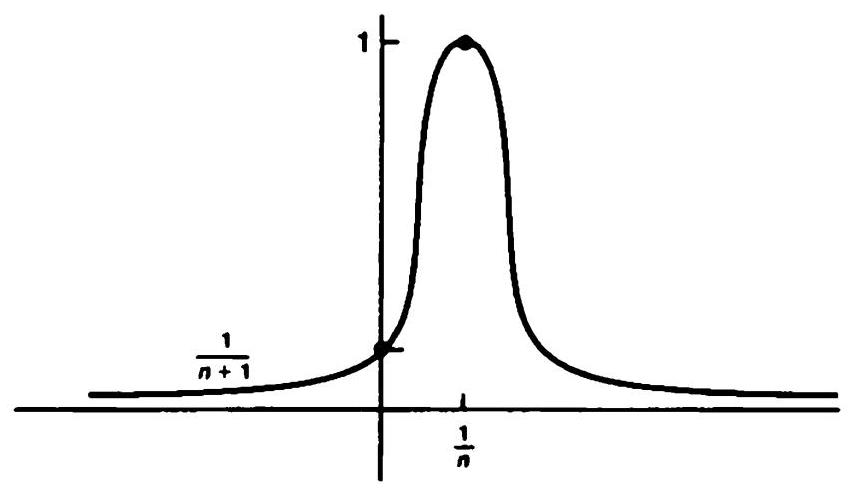
\includegraphics[width=0.7\textwidth]{images/21.1.jpg} \end{center} \hspace*{3em} Figure 21.1 The set \({B}^{2}\) is called the (closed) \index{Ball, unit} unit ball in \({\mathbb{R}}^{2}\) .
\item Prove the following standard facts about infinite series:
  \begin{enumerate}[itemsep=0.2em, parsep=0pt, topsep=0pt, partopsep=0pt, leftmargin=*, label=(\alph*), align=left]
  \item Show that if \(( {s}_{n})\) is a bounded sequence of real numbers and \({s}_{n} \leq  {s}_{n + 1}\) for each \(n\) , then \(( {s}_{n})\) converges.
  \item Let \(( {a}_{n})\) be a sequence of real numbers; define \[ {s}_{n} = \mathop{\sum }\limits_{{i = 1}}^{n}{a}_{i} \] If \({s}_{n} \rightarrow  s\) , we say that the infinite series \[ \mathop{\sum }\limits_{{i = 1}}^{\infty }{a}_{i} \] converges to \(s\) also. Show that if \(\sum {a}_{i}\) converges to \(s\) and \(\sum {b}_{i}\) converges to \(t\) , then \(\sum ( {c{a}_{i} + {b}_{i}})\) converges to \({cs} + t\) .
  \item Prove the comparison test for infinite series: If \(| {a}_{i}|  \leq  {b}_{i}\) for each \(i\) , and if the series \(\sum {b}_{i}\) converges, then the series \(\sum {a}_{i}\) converges. [Hint: Show that the series \(\sum | {a}_{i}|\) and \(\sum {c}_{i}\) converge, where \({c}_{i} = | {a}_{i}|  + {a}_{i}\) . \(\}\)
  \item Given a sequence of functions \({f}_{n} : X \rightarrow  \mathbb{R}\) , let \[ {s}_{n}( x)  = \mathop{\sum }\limits_{{i = 1}}^{n}{f}_{i}( x) . \] Prove the \index{Weierstrass M-test} Weierstrass \(M\) -test for uniform convergence: If \(| {{f}_{i}( x) }|  \leq  {M}_{i}\) for all \(x \in  X\) and all \(i\) , and if the series \(\sum {M}_{i}\) converges, then the sequence \(( {s}_{n})\) converges uniformly to a function \(s\) . [Hint: Let \({r}_{n} = \mathop{\sum }\limits_{{i = n + 1}}^{\infty }{M}_{i}\) . Show that if \(k > n\) , then \(| {{s}_{k}( x)  - {s}_{n}( x) }|  \leq  {r}_{n}\) ; conclude that \(| {s( x)  - {s}_{n}( x) }|  \leq  {r}_{n}\) .]
  \end{enumerate}
\item Prove continuity of the algebraic operations on \(\mathbb{R}\) , as follows: Use the metric \(d( {a,b})  = | {a - b}|\) on \(\mathbb{R}\) and the metric on \({\mathbb{R}}^{2}\) given by the equation \[ \rho ( {( {x,y}) ,( {{x}_{0},{y}_{0}}) })  = \max \{  {| {x - {x}_{0}}| ,| {y - {y}_{0}}| }\}  . \]
  \begin{enumerate}[itemsep=0.2em, parsep=0pt, topsep=0pt, partopsep=0pt, leftmargin=*, label=(\alph*), align=left]
  \item Show that addition is continuous. [Hint: Given \(\epsilon\) , let \(\delta  = \epsilon /2\) and note that \[ d( {x + y,{x}_{0} + {y}_{0}})  \leq  | {x - {x}_{0}}|  + | {y - {y}_{0}}| .\rbrack \]
  \item Show that multiplication is continuous. [Hint: Given \(( {{x}_{0},{y}_{0}})\) and \(0 < \epsilon  <\) 1, let \[ {3\delta } = \epsilon /( {| {x}_{0}|  + | {y}_{0}|  + 1}) \] and note that \[ d( {{xy},{x}_{0}{y}_{0}})  \leq  | {x}_{0}| | {y - {y}_{0}}|  + | {y}_{0}| | {x - {x}_{0}}|  + | {x - {x}_{0}}| | {y - {y}_{0}}| . \]
  \item Show that the operation of taking reciprocals is a continuous map from \(\mathbb{R} - \{ 0\}\) to \(\mathbb{R}\) . [Hint: Show the inverse image of the interval(a, b)is open. Consider five cases, according as \(a\) and \(b\) are positive, negative, or zero.]
  \item Show that the subtraction and quotient operations are continuous.
  \end{enumerate}
\end{enumerate}
\section*{*§ 22 The Quotient Topology \protect\sectionDagger}

Unlike the topologies we have already considered in this chapter, the \index{quotient topology} is not a natural generalization of something you have already studied in analysis. Nevertheless, it is easy enough to motivate. One motivation comes from geometry, where one often has occasion to use ``cut-and-paste'' techniques to construct such geometric objects as surfaces. The torus (surface of a doughnut), for example, can be constructed by taking a rectangle and ``pasting'' its edges together appropriately, as in Figure 22.1. And the sphere (surface of a ball) can be constructed by taking a disc and collapsing its entire boundary to a single point; see Figure 22 2. Formalizing these constructions involves the concept of quotient topology.

\begin{center}
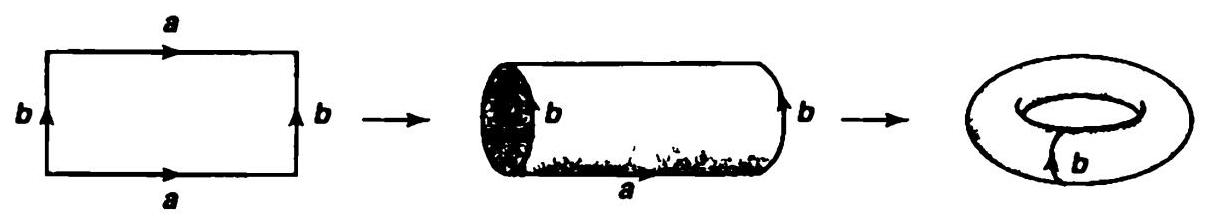
\includegraphics[width=1.0\textwidth]{images/22.1.jpg}
\end{center}
\hspace*{3em} 

Figure 22.1

\customfootnote{

${}^{\dagger}$ This section will be used throughout Part II of the book. It also is referred to in a number of exercises of Part I.

}

\begin{center}
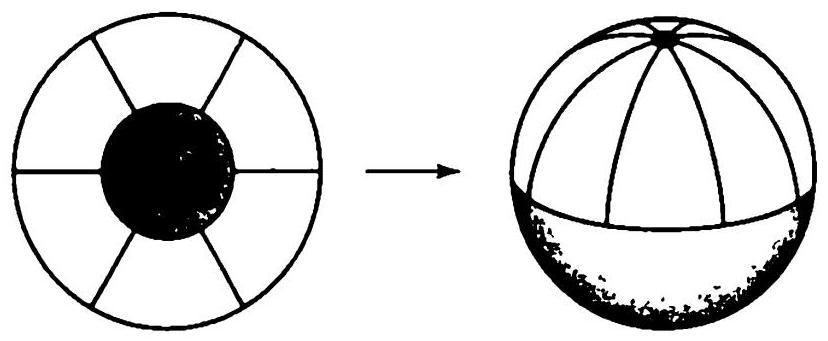
\includegraphics[width=0.7\textwidth]{images/22.2.jpg}
\end{center}
\hspace*{3em} 

Figure 22.2

\begin{definition}
	Let \(X\) and \(Y\) be topological spaces; let \(p : X \rightarrow  Y\) be a surjective map. The map \(p\) is said to be a \index{quotient map} provided a subset \(U\) of \(Y\) is open in \(Y\) if and only if \({p}^{-1}( U)\) is open in \(X\) .
\end{definition}

This condition is stronger than continuity; some mathematicians call it ``\index{strong continuity}.'' An equivalent condition is to require that a subset \(A\) of \(Y\) be closed in \(Y\) if and only if \({p}^{-1}( A)\) is closed in \(X\) . Equivalence of the two conditions follows from equation

\[
{f}^{-1}( {Y - B})  = X - {f}^{-1}( B) .
\]

Another way \index{Restriction: of a covering map!of a quotient map}of describing a \index{Quotient map}quotient map is as follows: We say that a subset \(C\) of \(X\) is \index{Saturated set} saturated (with respect to the surjective map \(p : X \rightarrow  Y\) ) if \(C\) contains every set \({p}^{-1}( {\{ y\} })\) that it intersects. Thus \(C\) is \index{saturated set@Saturated set}saturated if it equals the complete inverse image of a subset of \(Y\) . To say that \(p\) is a \index{Quotient map}quotient map is equivalent to saying that \(p\) is continuous and \(p\) maps saturated open sets of \(X\) to open sets of \(Y\) (or saturated \index{Closed set}closed sets of \(X\) to closed sets of \(Y\) ).

Two special kinds \index{Composite: of functions!of quotient maps}of quotient maps are the open maps and the \index{closed map}. Recall that a map \(f : X \rightarrow  Y\) is said to be an open map if for each open set \(U\) of \(X\) , the set \(f( U)\) is open in \(Y\) . It is said to be a closed map if for each closed set \(A\) of \(X\) , the set \(f( A)\) is closed in \(Y\) . It follows immediately from the definition that if \(p : X \rightarrow  Y\) is a surjective continuous map that is either open or closed, then \(p\) is a quotient map. There are quotient maps that are neither open nor closed. (See Exercise 3.)

\begin{centeredblock}
\begin{example}
	Let \(X\) be the subspace \([  {0,1}]   \cup  [  {2,3}]\) of \(\mathbb{R}\) , and let \(Y\) be the subspace \([  {0,2}]\) of \(\mathbb{R}\) . The map \(p : X \rightarrow  Y\) defined by

\[
p( x)  = \{  \begin{array}{ll} x & \text{ for }x \in  [  {0,1}]  , \\  x - 1 & \text{ for }x \in  [  {2,3}]   \end{array}.
\]

is readily seen to be surjective, continuous, and closed. Therefore it is a quotient map. It is not, however, an open map; the image of the open set \([  {0,1}]\) of \(X\) is not open \index{Closure!in a subspace}in \(Y\) .

Note that if \(A\) is the \index{Box topology!subspace}subspace \(\lbrack 0,1) \cup  [  {2,3}]\) of \(X\) , then the map \(q : A \rightarrow  Y\) obtained by restricting \(p\) \index{Projection map!is open map}is continuous and surjective, but it \index{Projection map!is open map}is not a quotient map. For the set \([  {2,3}]\) is open in \(A\) and is saturated with respect to \(q\) , but its image is not open in \(Y\) .
\end{example}
\end{centeredblock}

\begin{centeredblock}
\begin{example}
	Let \({\pi }_{1} : \mathbb{R} \times  \mathbb{R} \rightarrow  \mathbb{R}\) be projection onto the first coordinate; then \({\pi }_{1}\) is continuous and surjective. Furthermore, \({\pi }_{1}\) is an \index{Open map}open map. For if \(U \times  V\) is a nonempty basis element for \(\mathbb{R} \times  \mathbb{R}\) , then \({\pi }_{1}( {U \times  V})  = U\) is open in \(\mathbb{R}\) ; it follows that \({\pi }_{1}\) carries open sets of \(\mathbb{R} \times  \mathbb{R}\) to open sets of \(\mathbb{R}\) . However, \({\pi }_{1}\) is not a \index{Closed map}closed map. The subset

\[
C = \{ x \times  y \mid  {xy} = 1\}
\]

of \(\mathbb{R} \times  \mathbb{R}\) is closed, but \({\pi }_{1}( C)  = \mathbb{R} - \{ 0\}\) , which is not closed in \(\mathbb{R}\) .

Note that if \(A\) is the subspace of \(\mathbb{R} \times  \mathbb{R}\) that is the union of \(C\) and the origin \(\{ 0\}\) , then the map \(q \cdot  A \rightarrow  \mathbb{R}\) obtained by restricting \({\pi }_{1}\) is continuous and surjective, but it is not a \index{quotient map@Quotient map}quotient map. For the one-point set \(\{ \mathbf{0}\}\) is open in \(A\) and is saturated with respect to \(q\) , but its image is not open in \(\mathbb{R}\) .
\end{example}
\end{centeredblock}

Now we show how the notion of quotient map can be used to construct a topology on a set.

\begin{definition}
	If \(X\) is a space and \(A\) is a set and if \(p : X \rightarrow  A\) is a surjective map, then there exists exactly one topology \(\mathcal{T}\) on \(A\) relative to which \(p\) is a quotient map; it is called the quotient topology induced by \(p\) .
\end{definition}

The topology \(\mathcal{T}\) is of course defined by letting it consist of those subsets \(U\) of \(A\) such that \({p}^{-1}( U)\) is open in \(X\) . It is easy to check that \(\mathcal{T}\) is a topology. The sets \(\varnothing\) and \(A\) are open because \({p}^{-1}( \varnothing )  = \varnothing\) and \({p}^{-1}( A)  = X\) . The other two conditions follow from the equations

\[
{p}^{-1}( {\mathop{\bigcup }\limits_{{\alpha  \in  J}}{U}_{\alpha }})  = \mathop{\bigcup }\limits_{{\alpha  \in  J}}{p}^{-1}( {U}_{\alpha })
\]

\[
{p}^{-1}( {\mathop{\bigcap }\limits_{{i = 1}}^{n}{U}_{i}})  = \mathop{\bigcap }\limits_{{i = 1}}^{n}{p}^{-1}( {U}_{i})
\]

\begin{centeredblock}
\begin{example}
	Let \(p\) be the map of the real line \(\mathbb{R}\) onto the three-point set \(A = \{ a,b,c\}\) defined by

\[
p( x)  = \{  \begin{array}{ll} a & \text{ if }x > 0 \\  b & \text{ if }x < 0 \\  c & \text{ if }x = 0 \end{array}.
\]

You can check that the quotient topology on \(A\) induced by \(p\) is the one indicated in Figure 22.3

\begin{center}
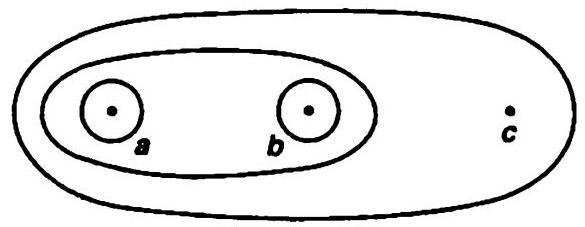
\includegraphics[width=0.5\textwidth]{images/22.3.jpg}
\end{center}
\hspace*{3em}

Figure 22.3
\end{example}
\end{centeredblock}

There is a special situation in which the quotient topology occurs particularly frequently. It is the following:

\begin{definition}
	Let \(X\) be a topological space, and let \({X}^{ * }\) be a partition of \(X\) into disjoint subsets whose union is \(X\) . Let \(p : X \rightarrow  {X}^{ * }\) be the surjective map that carries each point of \(X\) to the element of \({X}^{ * }\) containing it. In the \index{Quotient topology}quotient topology induced by \(p\) , the space \({X}^{ * }\) is called a quotient space of \(X\) .
\end{definition}

Given \({X}^{ * }\) , there is an equivalence relation on \(X\) of which the elements of \({X}^{ * }\) are the equivalence classes. One can think of \({X}^{ * }\) as having been obtained by ``ide ntifying'' each pair of equivalent points. \index{Hausdorff condition!for quotient space}For this reason, the quotient space \({X}^{ * }\) is often called an \index{identification space}, or a \index{decomposition space}, of the space \(X\) .

We can describe the topology of \({X}^{ * }\) in another way. A subset \(U\) of \({X}^{ * }\) is a collection of equivalence classes, and the set \({p}^{-1}( U)\) is just the union of the equivalence classes belongingg to \(U\) . Thus the typical open set of \({X}^{ * }\) is a collection of equivalence classes whose union is an open set of \(X\) .

\begin{centeredblock}
\begin{example}
	Let \(X\) be the closed unit ball

\[
\{  {x \times  y \mid  {x}^{2} + {y}^{2} \leq  1}\}
\]

in \({\mathbb{R}}^{2}\) , and let \({X}^{ * }\) be the partition of \(X\) consisting of all the one-point sets \(\{ x \times  y\}\) for which \({x}^{2} + {y}^{2} < 1\) , along with the set \({S}^{1} = \{ x \times  y\}  \mid  {x}^{2} + {y}^{2} = 1\}\) . Typical \index{saturated set@Saturated set}saturated open sets in \(X\) are pictured by the shaded regions in Figure 22.4. One can show that \({X}^{ * }\) is homeomorphic with the \index{Box topology!subspace}subspace of \({\mathbb{R}}^{3}\) called the unit 2-sphere, defined by

\[
\index{S@\({S}^{2}\)} {S}^{2} = \{  {( {x,y,z})  \mid  {x}^{2} + {y}^{2} + {z}^{2} = 1}\}  .
\]

\begin{center}
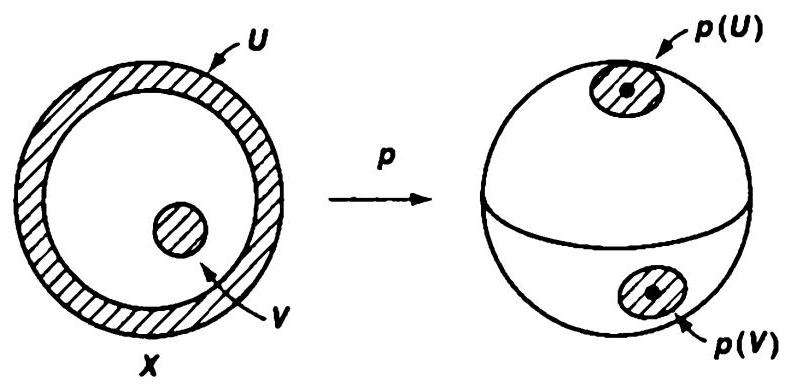
\includegraphics[width=0.7\textwidth]{images/22.4.jpg}
\end{center}
\hspace*{3em}

Figure 22.4
\end{example}
\end{centeredblock}

\begin{centeredblock}
\begin{example}
	Let \(X\) be the rectangle \([  {0,1}]   \times  [  {0,1}]\) . Define a partition \({X}^{ * }\) of \(X\) as follows: It consists of all the one-point sets \(\{ x \times  y\}\) where \(0 < x < 1\) and \(0 < y < 1\) , the following types of two-point sets:

\[
\{ x \times  0,x \times  1\} \;\text{ where }0 < x < 1,
\]

\[
\{ 0 \times  y,1 \times  y\} \;\text{ where }0 < y < 1,
\]

and the four-point set

\[
\{ 0 \times  0,0 \times  1,1 \times  0,1 \times  1\} .
\]

Typical saturated open sets in \(X\) are pictured by the shaded regions in Figure 22.5; each is an open set of \(X\) that equals a union of elements of \({X}^{ * }\) .

The image of each of these sets under \(p\) is an open set of \({X}^{ * }\) , as indicated in Figure 22.6. This description of \({X}^{ * }\) is just the mathematical way of saying what we expressed in pictures when we pasted the edges of a rectangle together to form a torus.
\end{example}
\end{centeredblock}

\begin{center}
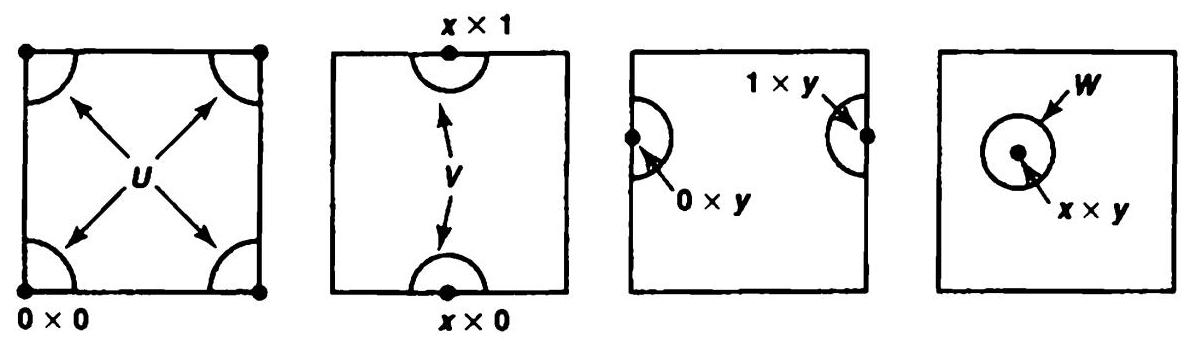
\includegraphics[width=1.0\textwidth]{images/22.5.jpg}
\end{center}
\hspace*{3em} 

Figure 22.5

\begin{center}
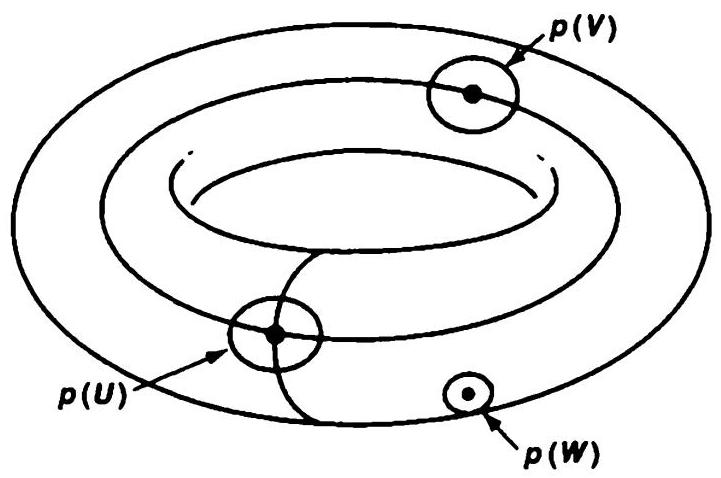
\includegraphics[width=0.6\textwidth]{images/22.6.jpg}
\end{center}
\hspace*{3em} 

Figure 22.6

Now we explore the relationship between the notions \index{Restriction: of a covering map!of a quotient map}of quotient map and quotient space and the concepts introduced previously. It is interesting to note that this relationship is not as simple as one might wish.

We have already noted that \index{Box topology!subspace}subspaces do not behave well; if \(p : X \rightarrow  Y\) is a quotient map and \(A\) is a subspace of \(X\) , then the map \(q : A \rightarrow  p( A)\) obtained by restricting \(p\) need not be a quotient map. One has, however, the following theorem:

\begin{theorem}
	Let \(p : X \rightarrow  Y\) be a quotient map; let \(A\) be a subspace of \(X\) that is saturated with respect to \(p\) ; let \(q : A \rightarrow  p( A)\) be the map obtained by restricting \(p\) .

(1) If \(A\) is either open or closed in \(X\) , then \(q\) is a quotient map.

*(2) If \(p\) is either an open map or a closed map, then \(q\) is a quotient map.

\end{theorem}
\begin{proof}
Step 1. We verify first the following two equations:

\[
{q}^{-1}( V)  = {p}^{-1}( V) \;\text{ if }V \subset  p( A)
\]

\[
p( {U \cap  A})  = p( U)  \cap  p( A) \;\text{ if }U \subset  X.
\]

To check the first equation, we note that since \(V \subset  p( A)\) and \(A\) is saturated, \({p}^{-1}( V)\) is contained in \(A\) . It follows that both \({p}^{-1}( V)\) and \({q}^{-1}( V)\) equal all points of \(A\) that are mapped by \(p\) into \(V\) . To check the second equation, we note that for any two subsets \(U\) \index{Sequences!and continuity}and \(A\) \index{Continuity: of algebraic operations in \(\mathbb{R}\)!of inclusion}of \(X\) , we have the inclusion

\[
p( {U \cap  A})  \subset  p( U)  \cap  p( A) \text{ . }
\]

To prove the reverse inclusion, suppose \(y = p( u)  = p( a)\) , for \(u \in  U\) and \(a \in  A\) . Since \(A\) is saturated, \(A\) contains the set \({p}^{-1}( {p( a) })\) , so that in particular \(A\) contains \(u\) . Then \(y = p( u)\) , where \(u \in  U \cap  A\) .

Step 2. Now suppose \(A\) is open or \(p\) is open. Given the subset \(V\) of \(p( A)\) , we assume that \({q}^{-1}( V)\) is open in \(A\) and show that \(V\) is open in \(p( A)\) .

Suppose first that \(A\) is open. Since \({q}^{-1}( V)\) is open in \(A\) and \(A\) is open in \(X\) , the set \({q}^{-1}( V)\) is open in \(X\) . Since \({q}^{-1}( V)  = {p}^{-1}( V)\) , the latter set is \index{open map@Open map}open in \(X\) , so that \(V\) is open in \(Y\) because \(p\) is a quotient map. In particular, \(V\) is open in \(p( A)\) .

Now suppose \(p\) is open. Since \({q}^{-1}( V)  = {p}^{-1}( V)\) and \({q}^{-1}( V)\) is open in \(A\) , we have \({p}^{-1}( V)  = U \cap  A\) for some set \(U\) open in \(X\) . Now \(p( {{p}^{-1}( V) })  = V\) because \(p\) is surjective; then

\[
V = p( {{p}^{-1}( V) })  = p( {U \cap  A})  = p( U)  \cap  p( A) .
\]

The set \(p( U)\) is open in \(Y\) because \(p\) is an \index{open map@Open map}open map; hence \(V\) is open in \(p( A)\) .

Step 3. The proof when \(A\) or \(p\) is closed is obtained by replacing the word ``open'' by the word ``closed'' throughout Step 2.

Now we consider other concepts introduced previously. \index{Quotient map!composites}Composites of maps behave nicely; it is easy to check that the composite of two quotient maps is a quotient map; this fact follows from the equation

\[
{p}^{-1}( {{q}^{-1}( U) })  = {( q \circ  p) }^{-1}( U) .
\]

On the other hand, \index{Quotient map!products}products of maps do not behave well; the cartesian product of two quotient maps need not be a quotient map. See Example 7 following. One needs further conditions on either the maps or the spaces in order for this statement to be true. One such, a condition on the spaces, is called local compactness; we shall study it later. Another, a condition on the maps, is the condition that both the maps \(p\) and \(q\) be open maps. In that case, it is easy to see that \(p \times  q\) is also an open map, so it is a quotient map.

Finally, the \index{Box topology!Hausdorff condition}Hausdorff condition does not behave well; even if \(X\) is Hausdorff. there is no reason that the quotient space \({X}^{ * }\) needs to be \index{Box topology!Hausdorff condition}Hausdorff. There is a simple condition for \({X}^{ * }\) to satisfy the \({T}_{1}\) axiom; one simply requires that each element of the partition \({X}^{ * }\) be a closed subset of \(X\) . Conditions that will ensure \({X}^{ * }\) is Hausdorff are harder to find. This is one of the more delicate questions concerning quotient spaces; we shall return to it several times later in the book.

Perhaps the most important result in the study of quotient spaces has to do with the problem \index{Composite: of functions!of continuous functions}of constructing continuous functions on a quotient space. We consider that problem now. When we studied \\index{Convergent sequence!in a product space}index{\index{product space@Product space}Product space}product spaces, we had a criterion for determining whether a map \(f : Z \rightarrow  \prod {X}_{\alpha }\) \index{Convergent sequence!in a product space}into a \index{product space@Product space}product space was continuous. Its counterpart in the theory of quotient spaces is a criterion for determining when a map \(f : {X}^{ * } \rightarrow  Z\) out of a quotient space is continuous. One has the following theorem:
\end{proof}

\begin{theorem}
	Let \(p : X \rightarrow  Y\) be a quotient map. Let \(Z\) be a space and let \(g : X \rightarrow  Z\) be a map that is constant on each set \({p}^{-1}( {\{ y\} })\) , for \(y \in  Y\) . Then \(g\) induces a map \(f : Y \rightarrow  Z\) such that \(f \circ  p = g\) . The induced map \(f\) is continuous if and only if \(g\) is continuous; \(f\) is a quotient map if and only if \(g\) is a quotient map.

\begin{center}
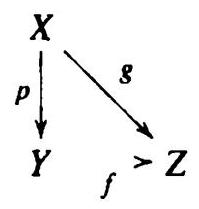
\includegraphics[width=0.2\textwidth]{images/22.7.jpg}
\end{center}
\hspace*{3em} 

\end{theorem}
\begin{proof}
For each \(y \in  Y\) , the set \(g( {{p}^{-1}( {\{ y\} }) })\) is a one-point set in \(Z\) (since \(g\) is constant on \({p}^{-1}( {\{ y\} }) )\) . If we let \(f( y)\) denote this point, then we have defined a map \(f : Y \rightarrow  Z\) such that for each \(x \in  X,f( {p( x) })  = g( x)\) . If \(f\) is continuous, then \(g = f \circ  p\) is continuous. Conversely, suppose \(g\) is continuous. Given an open set \(V\) of \(Z,{g}^{-1}( V)\) is open in \(X\) . But \({g}^{-1}( V)  = {p}^{-1}( {{f}^{-1}( V) })\) ; because \(p\) is a quotient map, it follows that \({f}^{-1}( V)\) is open in \(Y\) . Hence \(f\) is continuous.

If \(f\) is a quotient map, then \(g\) is the composite \index{Composite: of functions!of quotient maps}of two quotient maps and is thus a quotient map. Conversely, suppose that \(g\) is a quotient map. Since \(g\) is surjective, so is \(f\) . Let \(V\) be a subset of \(Z\) ; we show that \(V\) is open in \(Z\) if \({f}^{-1}( V)\) is open in \(Y\) . Now the set \({p}^{-1}( {{f}^{-1}( V) })\) is open in \(X\) because \(p\) is continuous. Since this set equals \({g}^{-1}( V)\) , the latter is open in \(X\) . Then because \(g\) is a quotient map, \(V\) is open in \(Z\) .
\end{proof}

\begin{corollary}
	Let \(g : X \rightarrow  Z\) be a surjective continuous map. Let \({X}^{ * }\) be the following collection of subsets of \(X\) :

\[
{X}^{ * } = \{  {{g}^{-1}( {\{ z\} })  \mid  z \in  Z}\}  .
\]

Give \({X}^{ * }\) the \index{Quotient topology}quotient topology.
\end{corollary}

(a) The map \(g\) induces a bijective continuous map \(f : {X}^{ * } \rightarrow  Z\) , which is a \index{Homeomorphism}homeomorphism if and only if \(g\) is a quotient map.

\begin{center}
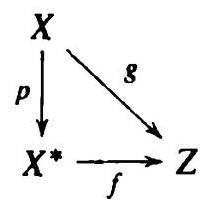
\includegraphics[width=0.2\textwidth]{images/22.8.jpg}
\end{center}
\hspace*{3em} 

(b) If \(Z\) is Hausdorff, so is \({X}^{ * }\) .

\begin{proof}
By the preceding theorem, \(g\) induces a continuous map \(f : {X}^{ * } \rightarrow  Z\) ; it is clear that \(f\) is bijective. Suppose that \(f\) is a \index{homeomorphism@Homeomorphism}homeomorphism. Then both \(f\) and the \index{Projection map}projection map \(p : X \rightarrow  {X}^{ * }\) are quotient maps, so that their composite \(q\) is a quotient map. Conversely, suppose that \(g\) is a quotient map Then it follows from the preceding theorem that \(f\) is a quotient map. Being bijective, \(f\) is thus a \index{homeomorphism@Homeomorphism}homeomorphism.

Suppose \(Z\) is Hausdorff. Given distinct pomts of \({X}^{ * }\) , their images under \(f\) are distinct and thus possess disjoint \index{Neighborhood}neighborhoods \(U\) and \(V\) . Then \({f}^{-1}( U)\) and \({f}^{-1}( V)\) are disjoint \index{neighborhood@Neighborhood}neighborhoods of the two given points of \({X}^{ * }\) .
\end{proof}

\begin{centeredblock}
\begin{example}
	Let \(X\) be the subspace of \({\mathbb{R}}^{2}\) that is the union of the line segments \([  {0,1}]   \times\)  \(\{ n\}\) , \index{Hausdorff condition!for subspace}for \(n \in  {\mathbb{Z}}_{ + }\) , and let \(Z\) be the subspace of \({\mathbb{R}}^{2}\) consisting of all points of the form \(x \times  ( {x/n})\) for \(x \in  [  {0,1}]\) and \(n \in  {\mathbb{Z}}_{ + }\) . Then \(X\) is the union of countably many disjoint line segments, and \(Z\) is the union of countably many line segments having an end point in common. See Figure 22.7.

Define a map \(g : X \rightarrow  Z\) by the equation \(g( {x \times  n})  = x \times  ( {x/n})\) ; then \(g\) is surjective and continuous. The quotient space \({X}^{ * }\) whose elements are the sets \({g}^{-1}( {\{ z\} })\) is simply the space obtained from \(X\) by identifying the subset \(\{ 0\}  \times  {\mathbb{Z}}_{ + }\) to a point. The map \(g\) induces a bijective continuous map \(f : {X}^{ * } \rightarrow  Z\) . But \(f\) is not a homeomorphism.

To verify this fact, it suffices to show that \(g\) is not a quotient map. Consider the sequence of points \({x}_{n} = ( {1/n})  \times  n\) of \(X\) . The set \(A = \{  {x}_{n}\}\) is a closed subset of \(X\) because it has no limut points. Also, it is saturated with respect to \(g\) On the other hand, the set \(g( A)\) is not closed in \(Z\) , for it consists of the points \({z}_{n} = ( {1/n})  \times  ( {1/{n}^{2}})\) ; this set has the origin as a \index{Limit point}limit point.

\begin{center}
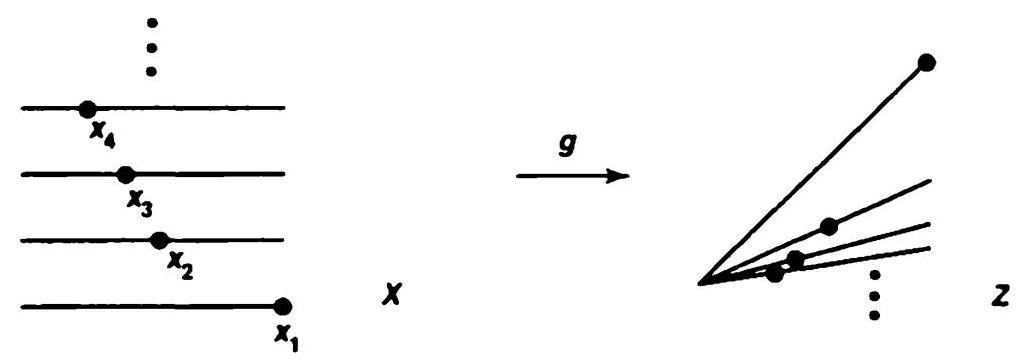
\includegraphics[width=0.9\textwidth]{images/22.9.jpg}
\end{center}
\hspace*{3em}

Figure 22.7
\end{example}
\end{centeredblock}

\begin{centeredblock}
\begin{example}
	The product of two quotient maps need not be a quotient map

We give an example that involves non-Hausdorff spaces in the exercises. Here is another involving spaces that are nicer.

Let \(X = \mathbb{R}\) and let \({X}^{ * }\) be the quotient space obtained from \(X\) by identifying the subset \({\mathbb{Z}}_{ + }\) to a point \(b\) ; let \(p : X \rightarrow  {X}^{ * }\) be the quotient map. Let \(\mathbb{Q}\) be the subspace of \(\mathbb{R}\) consisting of the rational numbers; let \(i : \mathbb{Q} \rightarrow  \mathbb{Q}\) be the identity map. We show that

\[
p \times  i : X \times  \mathbb{Q} \rightarrow  {X}^{ * } \times  \mathbb{Q}
\]

is not a quotient map.

For each \(n\) , let \({c}_{n} = \sqrt{2}/n\) , and c\index{Standard topology: on \(\mathbb{R}\)!on \({\mathbb{R}}^{2}\)}\index{Standard topology: on \(\mathbb{R}\)!on \({\mathbb{R}}^{2}\)}onsider the straight lines in \({\mathbb{R}}^{2}\) with slopes 1 and -1, respectively, through the point \(n \times  {c}_{n}\) Let \({U}_{n}\) consist of all points of \(X \times  \mathbb{Q}\) that lie above both of these lines or beneath both of them, and also between the vertical lines \(x = n - 1/4\) and \(x = n + 1/4\) . Then \({U}_{n}\) is open in \(X \times  \mathbb{Q}\) ; it contains the set \(\{ n\}  \times  \mathbb{Q}\) because \({c}_{n}\) is not rational. See Figure 22.8

Let \(U\) be the union of the sets \({U}_{n}\) ; then \(U\) is open in \(X \times  \mathbb{Q}\) . It is saturated with respect to \(p \times  i\) because it contains the enture set \({\mathbb{Z}}_{ + } \times  \{ q\}\) for each \(q \in  \mathbb{Q}\) . We assume that \({U}^{\prime } = ( {p \times  i}) ( U)\) is open in \({X}^{ * } \times  \mathbb{Q}\) and derive a contradiction

Because \(U\) contains, in particular, the set \({\mathbb{Z}}_{ + } \times  0\) , the set \({U}^{\prime }\) contains the point \(b \times  0\) . Hence \({U}^{\prime }\) contains an open set of the form \(W \times  {I}_{\delta }\) , where \(W\) is a \index{neighborhood@Neighborhood}neighborhood of \(b\) in \({X}^{ * }\) and \({l}_{\delta }\) consists of all rational numbers \(y\) with \(| y|  < \delta\) . Then

\[
{p}^{-1}( W)  \times  {I}_{\delta } \subset  U
\]

Choose \(n\) large enough that \({c}_{n} < \delta\) . Then since \({p}^{-1}( W)\) is open in \(X\) and contains \({\mathbb{Z}}_{ + }\) , we can choose \(\epsilon  < 1/4\) so that the interval \(( {n - \epsilon ,n + \epsilon })\) is contained in \({p}^{-1}( W)\) . Then \(U\) contains the subset \(V = ( {n - \epsilon ,n + \epsilon })  \times  {I}_{\delta }\) of \(X \times  \mathbb{Q}\) . But the figure makes clear that there are many points \(x \times  y\) of \(V\) that do not lie in \(U\) ! (One such is the point \(x \times  y\) , where \(x = n + \frac{1}{2}\epsilon\) and \(y\) is a rational number with \(| {y - {c}_{n}}|  < \frac{1}{2}\epsilon\) )

\begin{center}
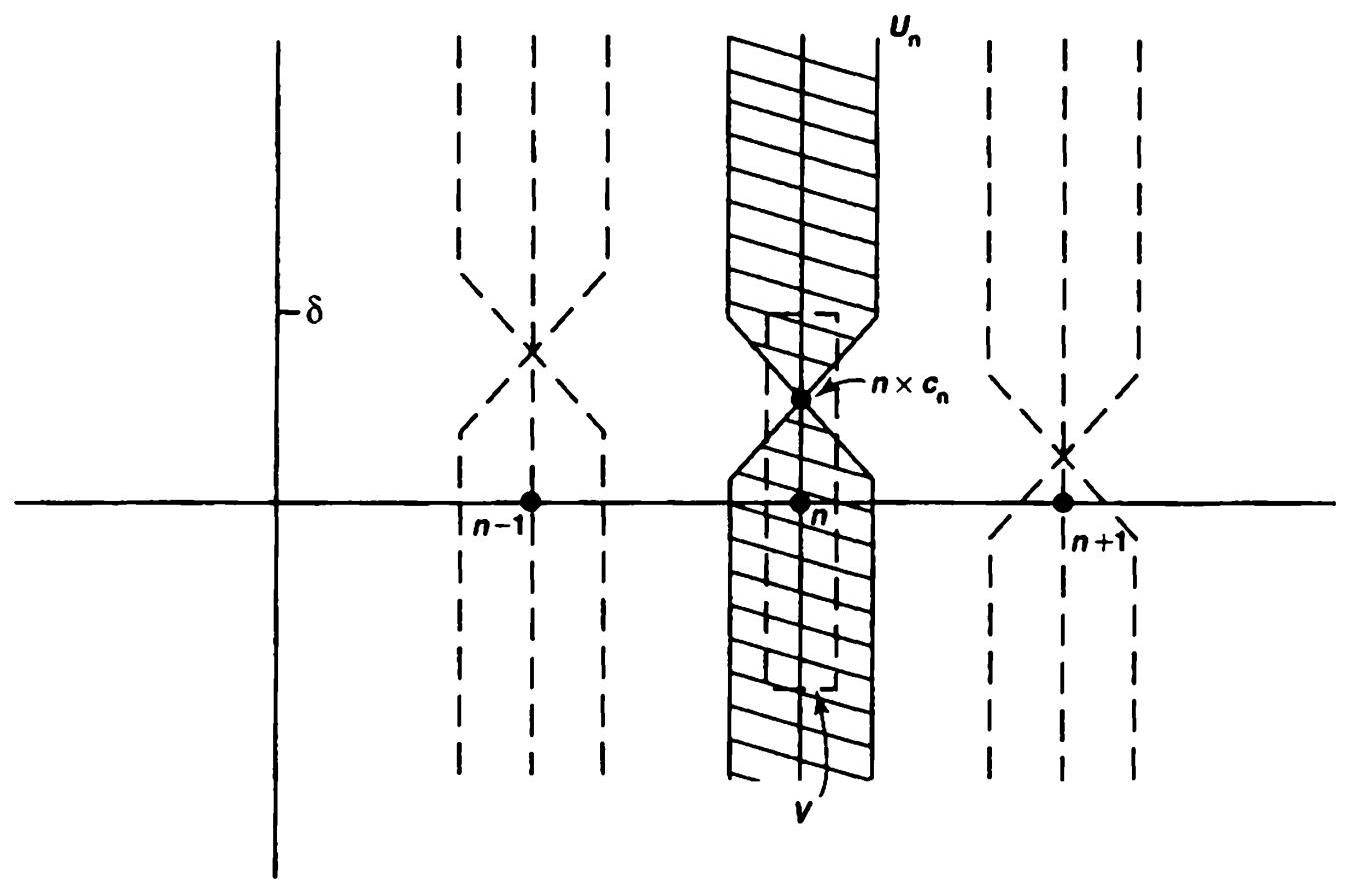
\includegraphics[width=1.0\textwidth]{images/22.10.jpg}
\end{center}
\hspace*{3em}

Figure 22.8
\end{example}
\end{centeredblock}

\section*{Exercises}
\begin{enumerate}[itemsep=0.4em, parsep=0pt, topsep=0pt, partopsep=0pt, leftmargin=*, label=\arabic*., ref=\arabic*]
\item Check the details of Example 3.
\item
  \begin{enumerate}[itemsep=0.2em, parsep=0pt, topsep=0pt, partopsep=0pt, leftmargin=*, label=(\alph*), align=left]
  \item Let \(p : X \rightarrow  Y\) be a continuous map. Show that if there is a continuous map \(f : Y \rightarrow  X\) such that \(p \circ  f\) equals the identity map of \(Y\) , then \(p\) is a quotient map.

  \item If \(A \subset  X\) , a retraction of \(X\) onto \(A\) is a continuous map \(r : X \rightarrow  A\) such that \(r( a)  = a\) for each \(a \in  A\) . Show that a retraction is a quotient map.
  \end{enumerate}
\item Let \({\pi }_{1} : \mathbb{R} \times  \mathbb{R} \rightarrow  \mathbb{R}\) be projection on the first coordinate Let \(A\) be the subspace of \(\mathbb{R} \times  \mathbb{R}\) consisting of all points \(x \times  y\) for which either \(x \geq  0\) or \(y = 0\) (or both); let \(q : A \rightarrow  \mathbb{R}\) be obtained by restricting \({\pi }_{1}\) . Show that \(q\) is a quotient map that is neither open nor closed.
\item
  \begin{enumerate}[itemsep=0.2em, parsep=0pt, topsep=0pt, partopsep=0pt, leftmargin=*, label=(\alph*), align=left]
  \item Define an equivalence relation on the plane \(X = {\mathbb{R}}^{2}\) as follows: \[ {x}_{0} \times  {y}_{0} \sim  {x}_{1} \times  {y}_{1}\;\text{ if }{x}_{0} + {y}_{0}^{2} = {x}_{1} + {y}_{1}^{2}. \] Let \({X}^{ * }\) be the corresponding quotient space. It is homeomorphic to a familiar space; what is it? [Hint: Set \(g( {x \times  y})  = x + {y}^{2}\) .]

  \item Repeat (a) for the equivalence relation \[ {x}_{0} \times  {y}_{0} \sim  {x}_{1} \times  {y}_{1}\;\text{ if }{x}_{0}^{2} + {y}_{0}^{2} = {x}_{1}^{2} + {y}_{1}^{2}. \]
  \end{enumerate}
\item Let \(p : X \rightarrow  Y\) be an open map. Show that if \(A\) is open in \(X\) , then the map \(q : A \rightarrow  p( A)\) obtained by restricting \(p\) is an open map.
\item Recall that \({\mathbb{R}}_{K}\) denotes the real line in the \(K\) -topology. (See \(§{13}\) .) Let \(Y\) be the quotient space obtained from \({\mathbb{R}}_{K}\) by collapsing the set \(K\) to a point; let \(p : {\mathbb{R}}_{K} \rightarrow  Y\) be the quotient map.
  \begin{enumerate}[itemsep=0.2em, parsep=0pt, topsep=0pt, partopsep=0pt, leftmargin=*, label=(\alph*), align=left]
  \item Show that \(Y\) satisfies the \({T}_{1}\) axiom, but is not Hausdorff.
  \item Show that \(p \times  p.{\mathbb{R}}_{K} \times  {\mathbb{R}}_{K} \rightarrow  Y \times  Y\) is not a quotient map. [Hint: The \index{Diagonal}diagonal is not closed in \(Y \times  Y\) , but its inverse image is closed in \({\mathbb{R}}_{K} \times  {\mathbb{R}}_{K}\) .]
  \end{enumerate}
\end{enumerate}
\section*{* Supplementary Exercises: Topological Groups}

In these exercises we consider topological groups and some of their properties. The quotient topology gets its name from the special case that arises when one forms the quotient of a topological group by a subgroup.

A topological group \(G\) is a group that is also a topological space satisfying the \({T}_{1}\) axiom, such that the map of \(G \times  G\) into \(G\) sending \(x \times  y\) into \(x \cdot  y\) , and the map of \(G\) into \(G\) sending \(x\) into \({x}^{-1}\) , are continuous maps. Throughout the following exercises, let \(G\) denote a topological group.

1. Let \(H\) denote a group that is also a topological space satisfying the \({T}_{1}\) axiom. Show that \(H\) is a topological group if and only if the map of \(H \times  H\) into \(H\) sending \(x \times  y\) into \(x \cdot  {y}^{-1}\) is continuous.

2. Show that the following are topological groups:

(a) \(( {\mathbb{Z}, + })\)

(b) \(( {\mathbb{R}, + })\)

(c) \(( {{\mathbb{R}}_{ + }, \cdot  })\)

(d) \(( {{S}^{1}, \cdot  })\) , where we take \({S}^{1}\) to be the space of all complex numbers \(z\) for which \(| z|  = 1\) .

(e) The general linear group \(\mathrm{{GL}}( n)\) , under the operation of matrix multiplication. (GL(n)is the set of all nonsingular \(n\) by \(n\) matrices, topologized by considering it as a subset of euclidean space of dimension \({n}^{2}\) in the obvious way.)

3. Let \(H\) be a subspace of \(G\) . Show that if \(H\) is also a subgroup of \(G\) , then both \(H\) and \(\bar{H}\) are topological groups.

4. Let \(\alpha\) be an element of \(G\) . Show that the maps \({f}_{\alpha },{g}_{\alpha } : G \rightarrow  G\) defined by

\[
{f}_{\alpha }( x)  = \alpha  \cdot  x\;\text{ and }\;{g}_{\alpha }( x)  = x \cdot  \alpha
\]

are homeomorphisms of \(G\) . Conclude that \(G\) is a homogeneous space. (This means that for every pair \(x,y\) of points of \(G\) , there exists a homeomorphism of \(G\) onto itself that carries \(x\) to \(y\) .)

5. Let \(H\) be a subgroup of \(G\) . If \(x \in  G\) , define \({xH} = \{ x \cdot  h \mid  h \in  H\}\) ; this set is called a left coset of \(H\) in \(G\) . Let \(G/H\) denote the collection of left cosets of \(H\) in \(G\) ; it is a partition of \(G\) . Give \(G/H\) the \index{quotient topology@Quotient topology}quotient topology.

(a) Show that if \(\alpha  \in  G\) , the map \({f}_{\alpha }\) of the preceding exercise induces a homeomorphism of \(G/H\) carrying \({xH}\) to \(( {\alpha  \cdot  x}) H\) . Conclude that \(G/H\) is a homogeneous space.

(b) Show that if \(H\) is a \index{closed set@Closed set}closed set in the topology of \(G\) , then one-point sets are \index{closed map@Closed map}closed in \(G/H\) .

(c) Show that the quotient map \(p : G \rightarrow  G/H\) is open.

(d) Show that if \(H\) is closed in the topology of \(G\) and is a \index{Norm}normal subgroup of \(G\) , then \(G/H\) is a topological group.

6. The integers \(\mathbb{Z}\) are a normal subgroup of \(( {\mathbb{R}, + })\) . The quotient \(\mathbb{R}/\mathbb{Z}\) is a familiar topological group; what is it?

7. If \(A\) and \(B\) are subsets of \(G\) , let \(A \cdot  B\) denote the set of all points \(a \cdot  b\) for \(a \in  A\) and \(b \in  B\) . Let \({A}^{-1}\) denote the set of all points \({a}^{-1}\) , for \(a \in  A\) .

(a) A neighborhood \(V\) of the identity element \(e\) is said to be sym\index{Metric}metric if \(V =\)  \({V}^{-1}\) . If \(U\) is a neighborhood of \(e\) , show there is a sym\index{metric@Metric}metric neighborhood \(V\) of \(e\) such that \(V \cdot  V \subset  U\) . [Hint: If \(W\) is a neighborhood of \(e\) , then \(W \cdot  {W}^{-1}\) is symmetric.]

(b) Show that \(G\) is Hausdorff. In fact, show that if \(x \neq  y\) , there is a neighborhood \(V\) of \(e\) such that \(V \cdot  x\) and \(V \cdot  y\) are disjoint.

(c) Show that \(G\) satisfies the following separation axiom, which is called the regularity axiom: Given a \index{closed set@Closed set}closed set \(A\) and a point \(x\) not in \(A\) , there exist disjoint open sets containing \(A\) and \(x\) , respectively. [Hint: There is a neighborhood \(V\) of \(e\) such that \(V \cdot  x\) and \(V \cdot  A\) are disjoint.]

(d) Let \(H\) be a subgroup of \(G\) that is closed in the topology of \(G\) ; let \(p : G \rightarrow\)  \(G/H\) be the quotient map. Show that \(G/H\) satisfies the regularity axiom. [Hint. Examine the proof of (c) when \(A\) is saturated.]